\documentclass[12pt,american]{report}
\usepackage{times}
\usepackage[T1]{fontenc}
\usepackage[utf8]{inputenc}
\usepackage{graphicx}
\usepackage{geometry}
\usepackage{siunitx}
\usepackage{pgfplots}
\geometry{verbose,letterpaper,tmargin=1in,bmargin=1in,lmargin=1.5in,rmargin=1in} %% sets paper size and margins
\usepackage{setspace}

\usepackage[square]{natbib}
\bibliographystyle{unsrtnat}


%\singlespacing        %% 1-spacing (default)
%\onehalfspacing       %% 1,5-spacing
%\doublespacing        %% 2-spacing

\pagestyle{plain}      %% select plain page style: no headers, page numbers center bottom

%% uncomment the following to include headers (e.g., to keep track of draft versions). Also change pagestyle to fancyplain:
%\rhead[\fancyplain{}{\leftmark}]%0
%      {\fancyplain{}{Draft 04/08 -- \thepage}}
%\cfoot[\fancyplain{Draft 04/08 -- \thepage}{}]{\fancyplain{Draft 04/08 -- \thepage}{}}

\begin{document}

\pagenumbering{roman}        %% roman page numbers for front matter

\renewcommand\thepage{}
\pagestyle{plain}
\begin{center}
\textbf{FRAMESHIFT: SHIFT YOUR ATTENTION, SHIFT THE STORY}
\vspace{0.4cm}

A Thesis\\ [0.4cm]
Submitted to the Faculty \\ [0.4cm]
in partial fulfillment of the requirements for the \\[0.4cm]
degree of \\[0.4cm]
Master of Science\\in\\Computer Science with a Concentration in Digital Arts\\[0.4cm]
by\\[0.5cm]
Tim Tregubov\\[0.4cm]
in Conjunction with Rukmini Goswami \\[0.5cm]
Department of Computer Science \\ [0.4cm]
DARTMOUTH COLLEGE \\ [0.4cm]
Hanover, New Hampshire \\[0.4cm]
May 15, 2015 % that you will submit your signed thesis
\vspace{1.5cm}

\end{center}

Examining Committee:

\begin{flushright}
Chair \line(180, 0){110} \\
Lorie Loeb\\[1cm]

Member \line(180, 0){110} \\
Michael Cohen \\[1cm]

Member \line(180, 0){110} \\
Michael Casey \\[1cm]

% Member \line(180, 0){110} \\
% MEMBER NAME HERE\\[1cm]

%(ALL signatures must be in Black ink, ALL fonts in black ink)

\end{flushright}

\begin{flushleft}
\line(180, 0){110} \\
F. Jon Kull, Ph.D.\\
Dean of Graduate Studies\\[1cm]
%NOTE: the copies you submit must have the original signatures for PhD, one hard copy, for MS, two copies and a pdf of the thesis is required for both degrees.  No Holes, clips or binding on the copy and should be on Quality paper, preferably, Dartmouth Bond.
\end{flushleft}







\pagestyle{plain}
\begin{center}
\textbf{FRAMESHIFT: SHIFT YOUR ATTENTION, SHIFT THE STORY}
\vspace{0.4cm}

A Thesis\\ [0.4cm]
Submitted to the Faculty \\ [0.4cm]
in partial fulfillment of the requirements for the \\[0.4cm]
degree of \\[0.4cm]
Master of Science\\in\\Computer Science with a Concentration in Digital Arts\\[0.4cm]
by\\[0.5cm]
Rukmini Goswami\\[0.4cm]
in Conjunction with Tim Tregubov \\[0.5cm]
Department of Computer Science \\ [0.4cm]
DARTMOUTH COLLEGE \\ [0.4cm]
Hanover, New Hampshire \\[0.4cm]
May 15, 2015 % that you will submit your signed thesis
\vspace{1.5cm}

\end{center}

Examining Committee:

\begin{flushright}
Chair \line(180, 0){110} \\
Lorie Loeb\\[1cm]

Member \line(180, 0){110} \\
Michael Cohen \\[1cm]

Member \line(180, 0){110} \\
Michael Casey \\[1cm]

% Member \line(180, 0){110} \\
% MEMBER NAME HERE\\[1cm]

%(ALL signatures must be in Black ink, ALL fonts in black ink)

\end{flushright}

\begin{flushleft}
\line(180, 0){110} \\
F. Jon Kull, Ph.D.\\
Dean of Graduate Studies\\[1cm]
%NOTE: the copies you submit must have the original signatures for PhD, one hard copy, for MS, two copies and a pdf of the thesis is required for both degrees.  No Holes, clips or binding on the copy and should be on Quality paper, preferably, Dartmouth Bond.
\end{flushleft}







\newpage
% a blank page follows the title page, this page is not numbered
\mbox{}
\newpage

\renewcommand\thepage{\arabic{page}}
\pagenumbering{roman}        %% roman page numbers for front matterstarting with page ii
\setcounter{page}{2}


% \renewcommand\thechapter{\arabic{chapter}.}
\renewcommand\thesection{\Roman{section}.}
\renewcommand\thesubsection{(\alph{subsection})}

\doublespacing               %% set spacing to double

\pagestyle{plain}
\begin{center}


\section*{ABSTRACT}


\end{center}
Crafting a 3D paper pop-up can be a lot of fun, and can help develop spatial reasoning skills.  However, designing the cuts and folds is often a frustrating trial and error process.  Foldlings is an iPad application that assists in this exploratory process.   Our tool-based approach allows users of all skill levels to create complex cards with ease, separating folding geometries into logical units.  This thesis focusses on the user interface and algorithms used in creating the two-dimensional view of the popup card from user input.

\cleardoublepage

\pagestyle{plain}
\begin{center}


\section*{Acknowledgements}

Thanks to Marissa Allen, my collaborator on this project, and co-author of chapters X and Y. \\
Tim Tregubov \\
Thanks also to our advisors: Jodie Mack, Lorie Loeb, and Emily Whiting \\
Thanks to our first user: Rukmini Goswami. \\

\end{center}



\cleardoublepage


\singlespacing
\tableofcontents             %% include TOC
\listoftables                %% include list of tables
\listoffigures               %% include list of figures
\cleardoublepage             %% start new page

\pagenumbering{arabic}       %% arabic page numbers for body of text starting with page 1

\doublespacing
% \include{Introduction}

 \include{chapters/Development_Methodology}
 \section{TODO}\label{todo}

todo

 \section{TODO}\label{todo}

sfsfs

 \section{TODO}\label{todo}

fdsf

 \section{TODO}\label{todo}

sfds

 \section{TODOsf}\label{todosf}

sfds

 \section{TODO}\label{todo}

fdsfsd

 \section{Interface Data Structures}\label{interface-data-structures}

\subsection{Edges}\label{edges}

An Edge represents a cut or fold. Edges are the basic building block of
planes and

\subsubsection{Driving Folds}\label{driving-folds}

A driving fold is not a special type of edge, but rather a . Any fold
can be the driving fold for

\subsection{Planes}\label{planes}

A plane is a list of Edges. \textbf{TODO: CITE MARISSA HERE}

\subsection{Fold Features}\label{fold-features}

The central data structure of Foldlings is the FoldFeature: a
representation of a shape drawn by the user that folds in 3d. Each fold
feature is a single design element ---~and can be individually created,
modified, and deleted. There are five types of FoldFeature: MasterCard,
BoxFold, FreeForm, Polygon, and V-Fold, representing differences in
drawing behavior, geometry, and (the differences are described in detail
below). Each of these features is a subclass of the FoldFeature super
class.

All FoldFeatures have functionality in common:

\begin{itemize}
\itemsep1pt\parskip0pt\parsep0pt
\item
  Each feature contains a list of edges in the feature ---~both cuts and
  folds
\item
  Each feature has a driving fold --- in the case of unconnected
  features, such as the master card and holes, the driving fold is nil.
\item
  Each feature can be deleted from the Sketch, ``healing'' the sketch by
  closing gaps left in any
\item
  Features implement the encodeWithCoder and decodeWithCoder methods,
  allowing them to be serialized to a file on the device and restored
  from the saved file.
\item
  Each feature can provide a list of current ``tap options'' --- actions
  that can be performed on the feature given its state. \textbf{TODO:SEE
  tap options in interface design} \citep{Nobody06}. \textbf{TODO:REMOVE
  -- JUST TESTING}
\end{itemize}

In addition, each feature contains

\subsubsection{MasterCard}\label{mastercard}

\subsubsection{Box Fold}\label{box-fold}

\subsubsection{FreeForm}\label{freeform}

Holes are a special case of FreeForm shapes. FreeForm shapes that do not
cross a fold are considered holes ---~drawn in white in the 2d sketch
and drawn as subtractions from planes in the 3d view.

\subsubsection{Polygon}\label{polygon}

\subsubsection{V-Fold}\label{v-fold}

\subsubsection{Validity}\label{validity}

 \textbf{TODO: include preliminary user study 1}

sfdaf

 \section{TODOfds}\label{todofds}

afsdfs dsf sf

 \section{TODO23}\label{todo23}

fdjas

 \section{User Test at the Digital Arts
Exhibition}\label{user-test-at-the-digital-arts-exhibition}

On April 28, 2015, we tested our system with attendees of the Digital
Arts Exhibition at Dartmouth. After a brief demonstration of how to
create folds and preview their design, users designed cards using
Foldlings. Users drew sketches and then sent an email containing an SVG
file to the computer connected to the laser cutter. Finally, they placed
a piece of paper in the laser cutter, and watched as the laser beam cut
out their design. Over the course of two hours, users cut and folded 31
popup cards. \textless{}\textless{}TOOO: CITE DAX
\textless{}\textless{}TODO:

The system we demonstrated at the exhibition was incomplete --- it
contained the basic box fold and freeform shape tools, but did not
include some advanced features of the final software, such as dragging
folds or shading based on plane orientation. The alpha software also
contained several bugs that disrupted the experience. However, the
system was usable enough for people to create cards, and observing user
behavior was invaluable in designing our final product.

Because users were new to our system --- and constrained by the pressure
of other users waiting to design cards --- designs were relatively
simple. Sketches generally contained between 2 and 5 fold features in
addition to the base card --- the most complex design contained 10 fold
features. Despite their simplicity, sketches showed a wide range of
designs, ranging from abstract shapes to representational scenes ---
users sketched symbols, Chinese characters, and geometric forms. Most of
the sketches utilized both freeform and box fold features, mixing the
two element types to create a composition. One of the most popular
design elements was the user's name: 5 of the cards contained names or
initials. Roughly a third of the designs took advantage of nesting ---
constructing fold features inside each other.

Because users were able to quickly design and fabricate their design,
people generally left satisfied. People typically spent around 20
minutes at our booth, leaving with a popup card they had created.
However, the experience was not frictionless. Users were frustrated by
crashes: touching the screen with more than one finger or drawing while
calculating planes were the most common reasons for failure. Other
common complaints were the lack of a delete/undo button and that the UI
did not show which tool was currently selected.

Folding the fabricated design also presented difficulties. Although they
were able to see a 3d preview of their design while creating it, users
had often relinquished the iPad by the time they folded their design.
They were often unsure how to fold their card, and struggled to discover
the correct fold orientations. In some cases, it took longer for users
to fold their creation than to design it.

We observed several unexpected behaviors. A few users rotated the screen
to design a card in a landscape view, rather than the portrait
orientation implied by the orientation of the buttons and 3d preview.
They used this orientation to design cards that folded medially rather
than laterally. Several users also constructed overlapping features by
drawing on top of existing features. These features did not simulate
correctly, as they intersected with existing edges. However, this
behavior demonstrated a desire to construct more complex geometry. In
the final software we implement unions for fold features --- the most
recently-drawn feature occludes features underneath it, modifying their
edges.

Users also relied on the 3d preview to differing degrees. Some users
viewed the preview after every operation, while others only switched to
the preview occasionally. Many users relied on the 3d preview as a
reference to how to fold their popup card. We were surprised by this,
and conducted further user studies to determine the effectiveness of
methods of displaying 3d information.

 \section{Final User Study}\label{final-user-study}

As a final test of software, we compared the effectiveness of .

The study comprised two components:

\textbf{\textgreater{}\textgreater{}TODO: update}

\section{TODO}\label{todo}

goal: test whether users understand the mapping of 2d fold patterns to
3d, and test the degree to which plane coloring, edge patterning, and a
3d preview help users understand how a popup card will fold.

Each subject received a set of five laser cut cards, and we recorded the
time it takes them to successfully fold the card.

For each card, each subject was randomly given one of of the following
five aids:

\begin{enumerate}
\def\labelenumi{\arabic{enumi})}
\itemsep1pt\parskip0pt\parsep0pt
\item
  A two-dimensional design, showing planes shaded by whether they will
  be horizontal or vertical when folded.
\item
  A two-dimensional design, with edges patterned based on whether they
  are ``hills'' or ``valleys'' --- whether they fold towards or away
  from the card.
\item
  A video showing a simulation of the card folding in three dimensions.
\item
  A still image of the card folded in dimension.
\item
  No visual aid.
\end{enumerate}

The order of aids was shuffled randomly, and then balanced to ensure an
equal distribution of orderings. I.e. each

Finally, we asked subjects to rank the visual aids

The effect each type of aid has on folding time will help determine
which types of visualization to include in Foldlings


%\include{Chapter2}          % continue to include all the chapters.

\appendix


\section*{Appendix A: User Study 1}
\addcontentsline{toc}{section}{Appendix A: User Study 1}

% \begin{figure}[h!]
% \begin{center}$
% \begin{array}{c c}
% 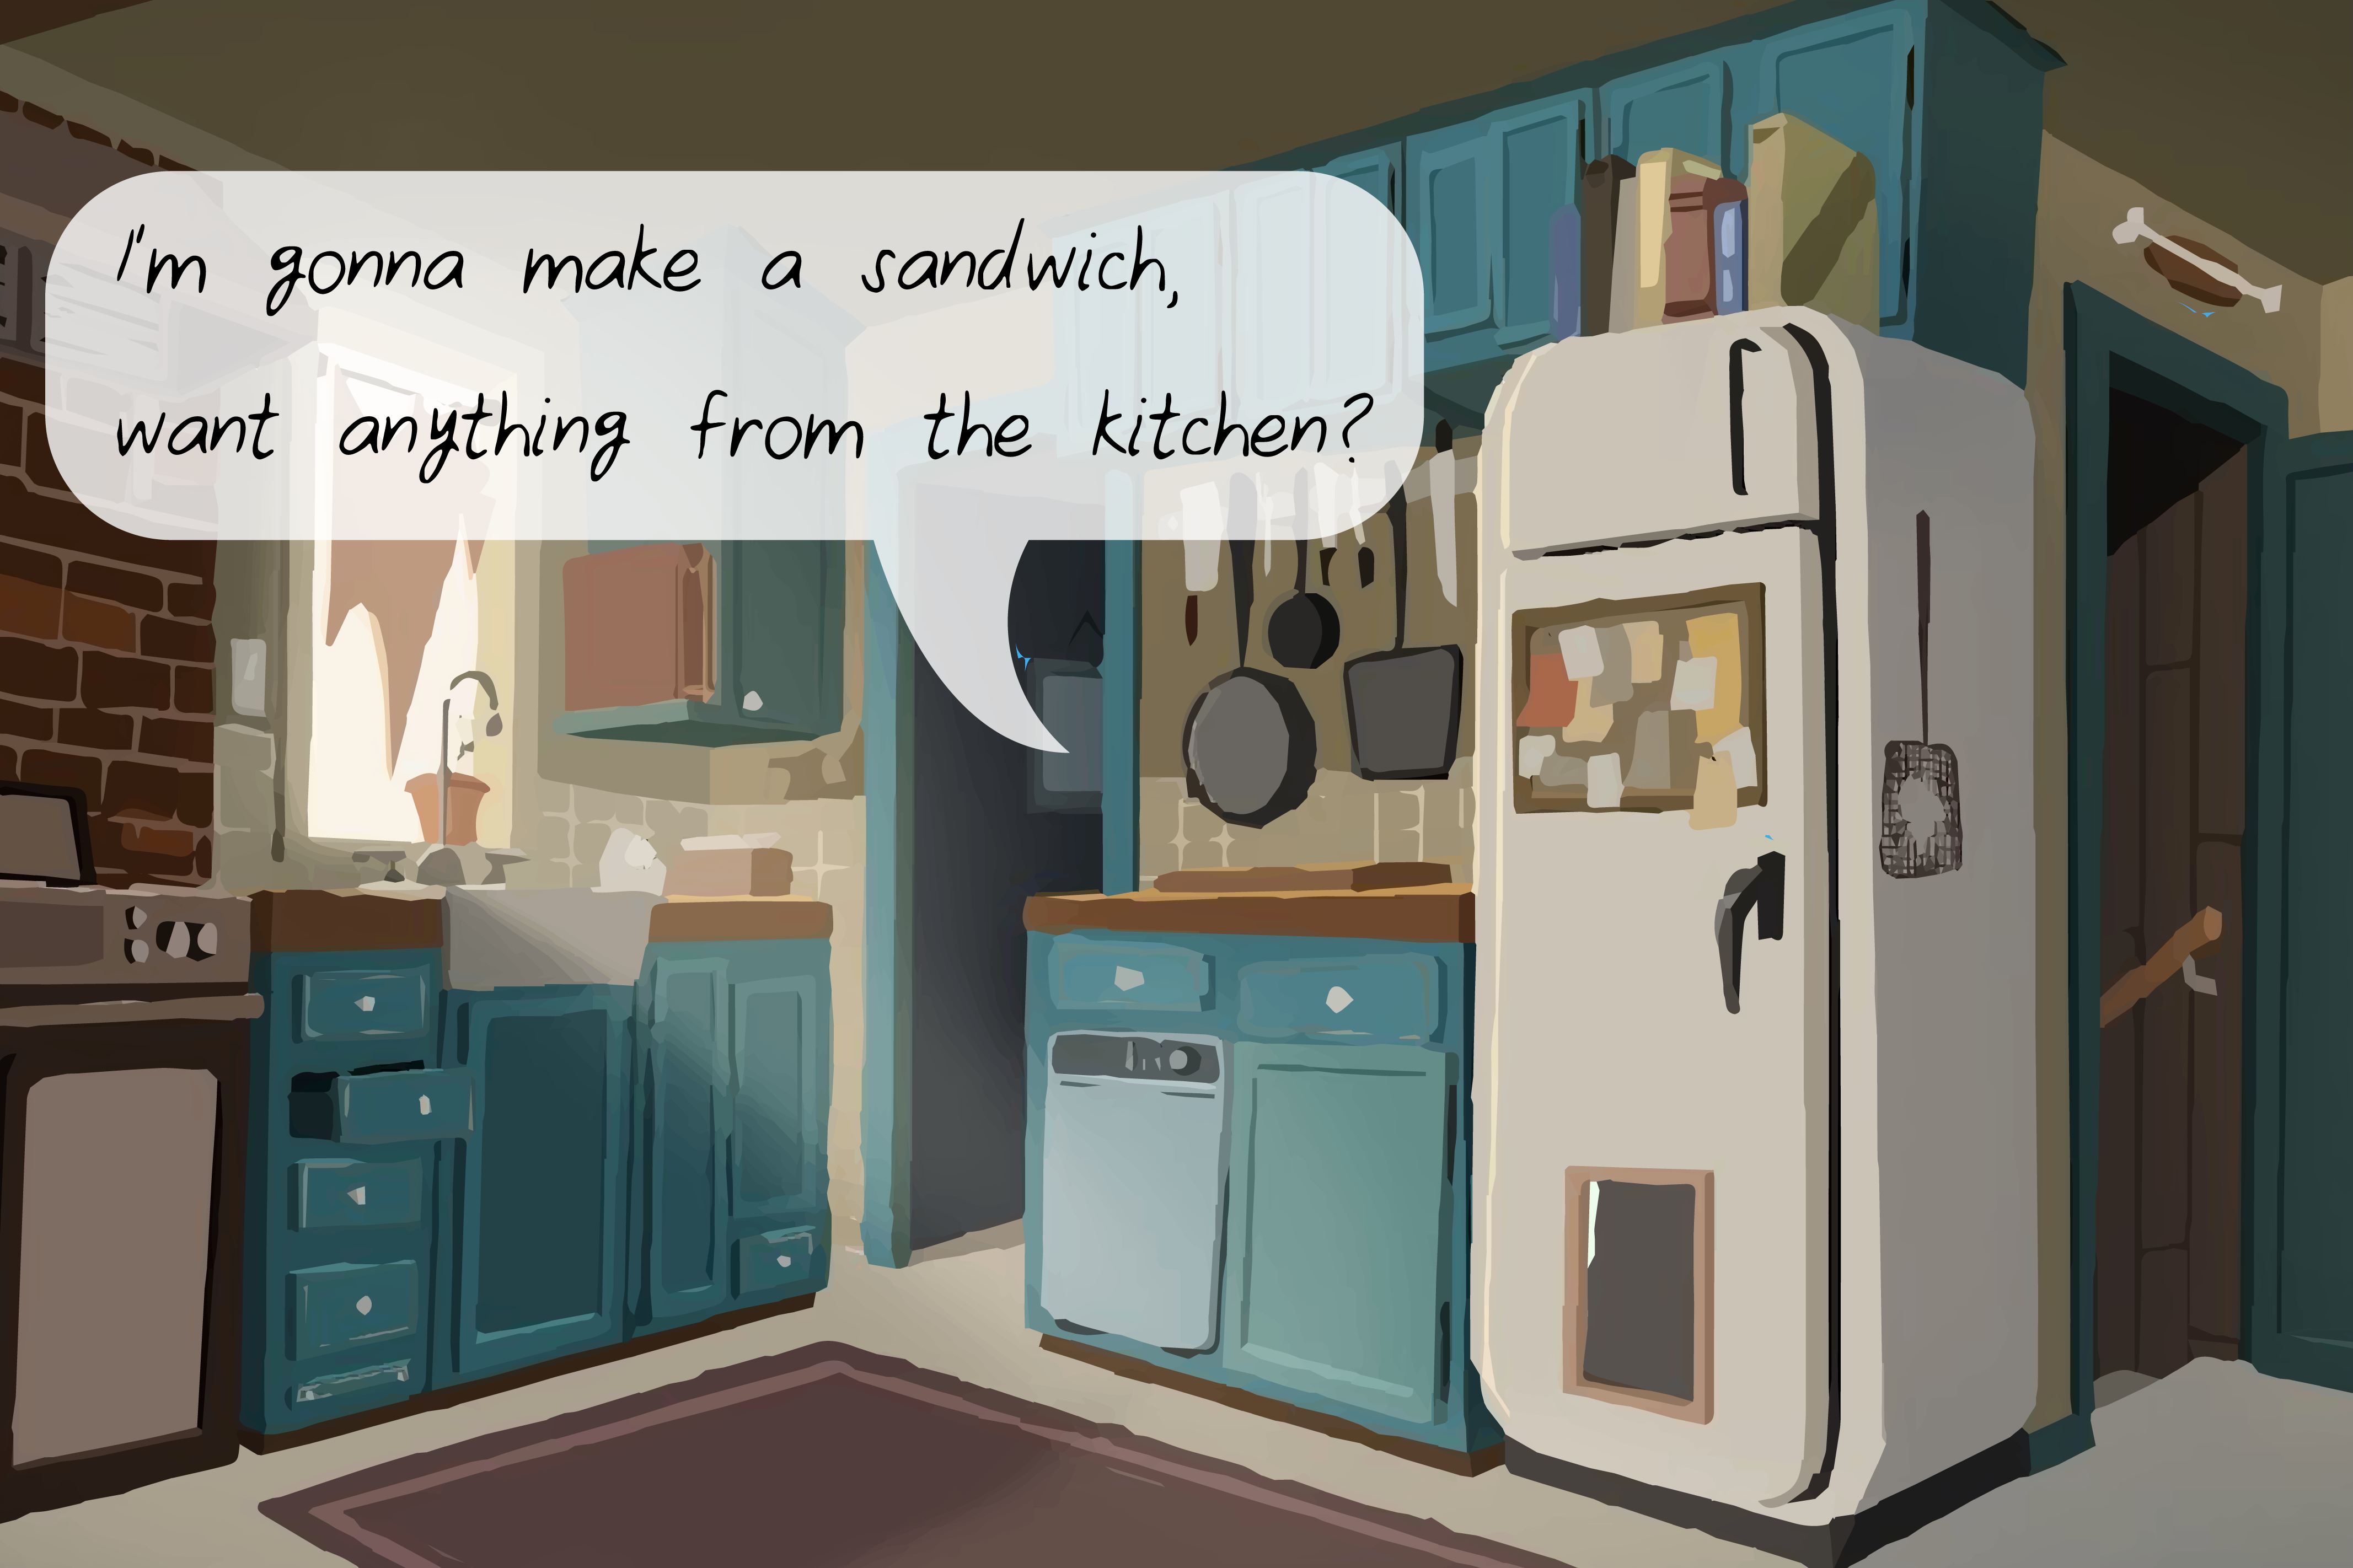
\includegraphics[width=2.3in]{figures/exp1/test-01.png} &
% 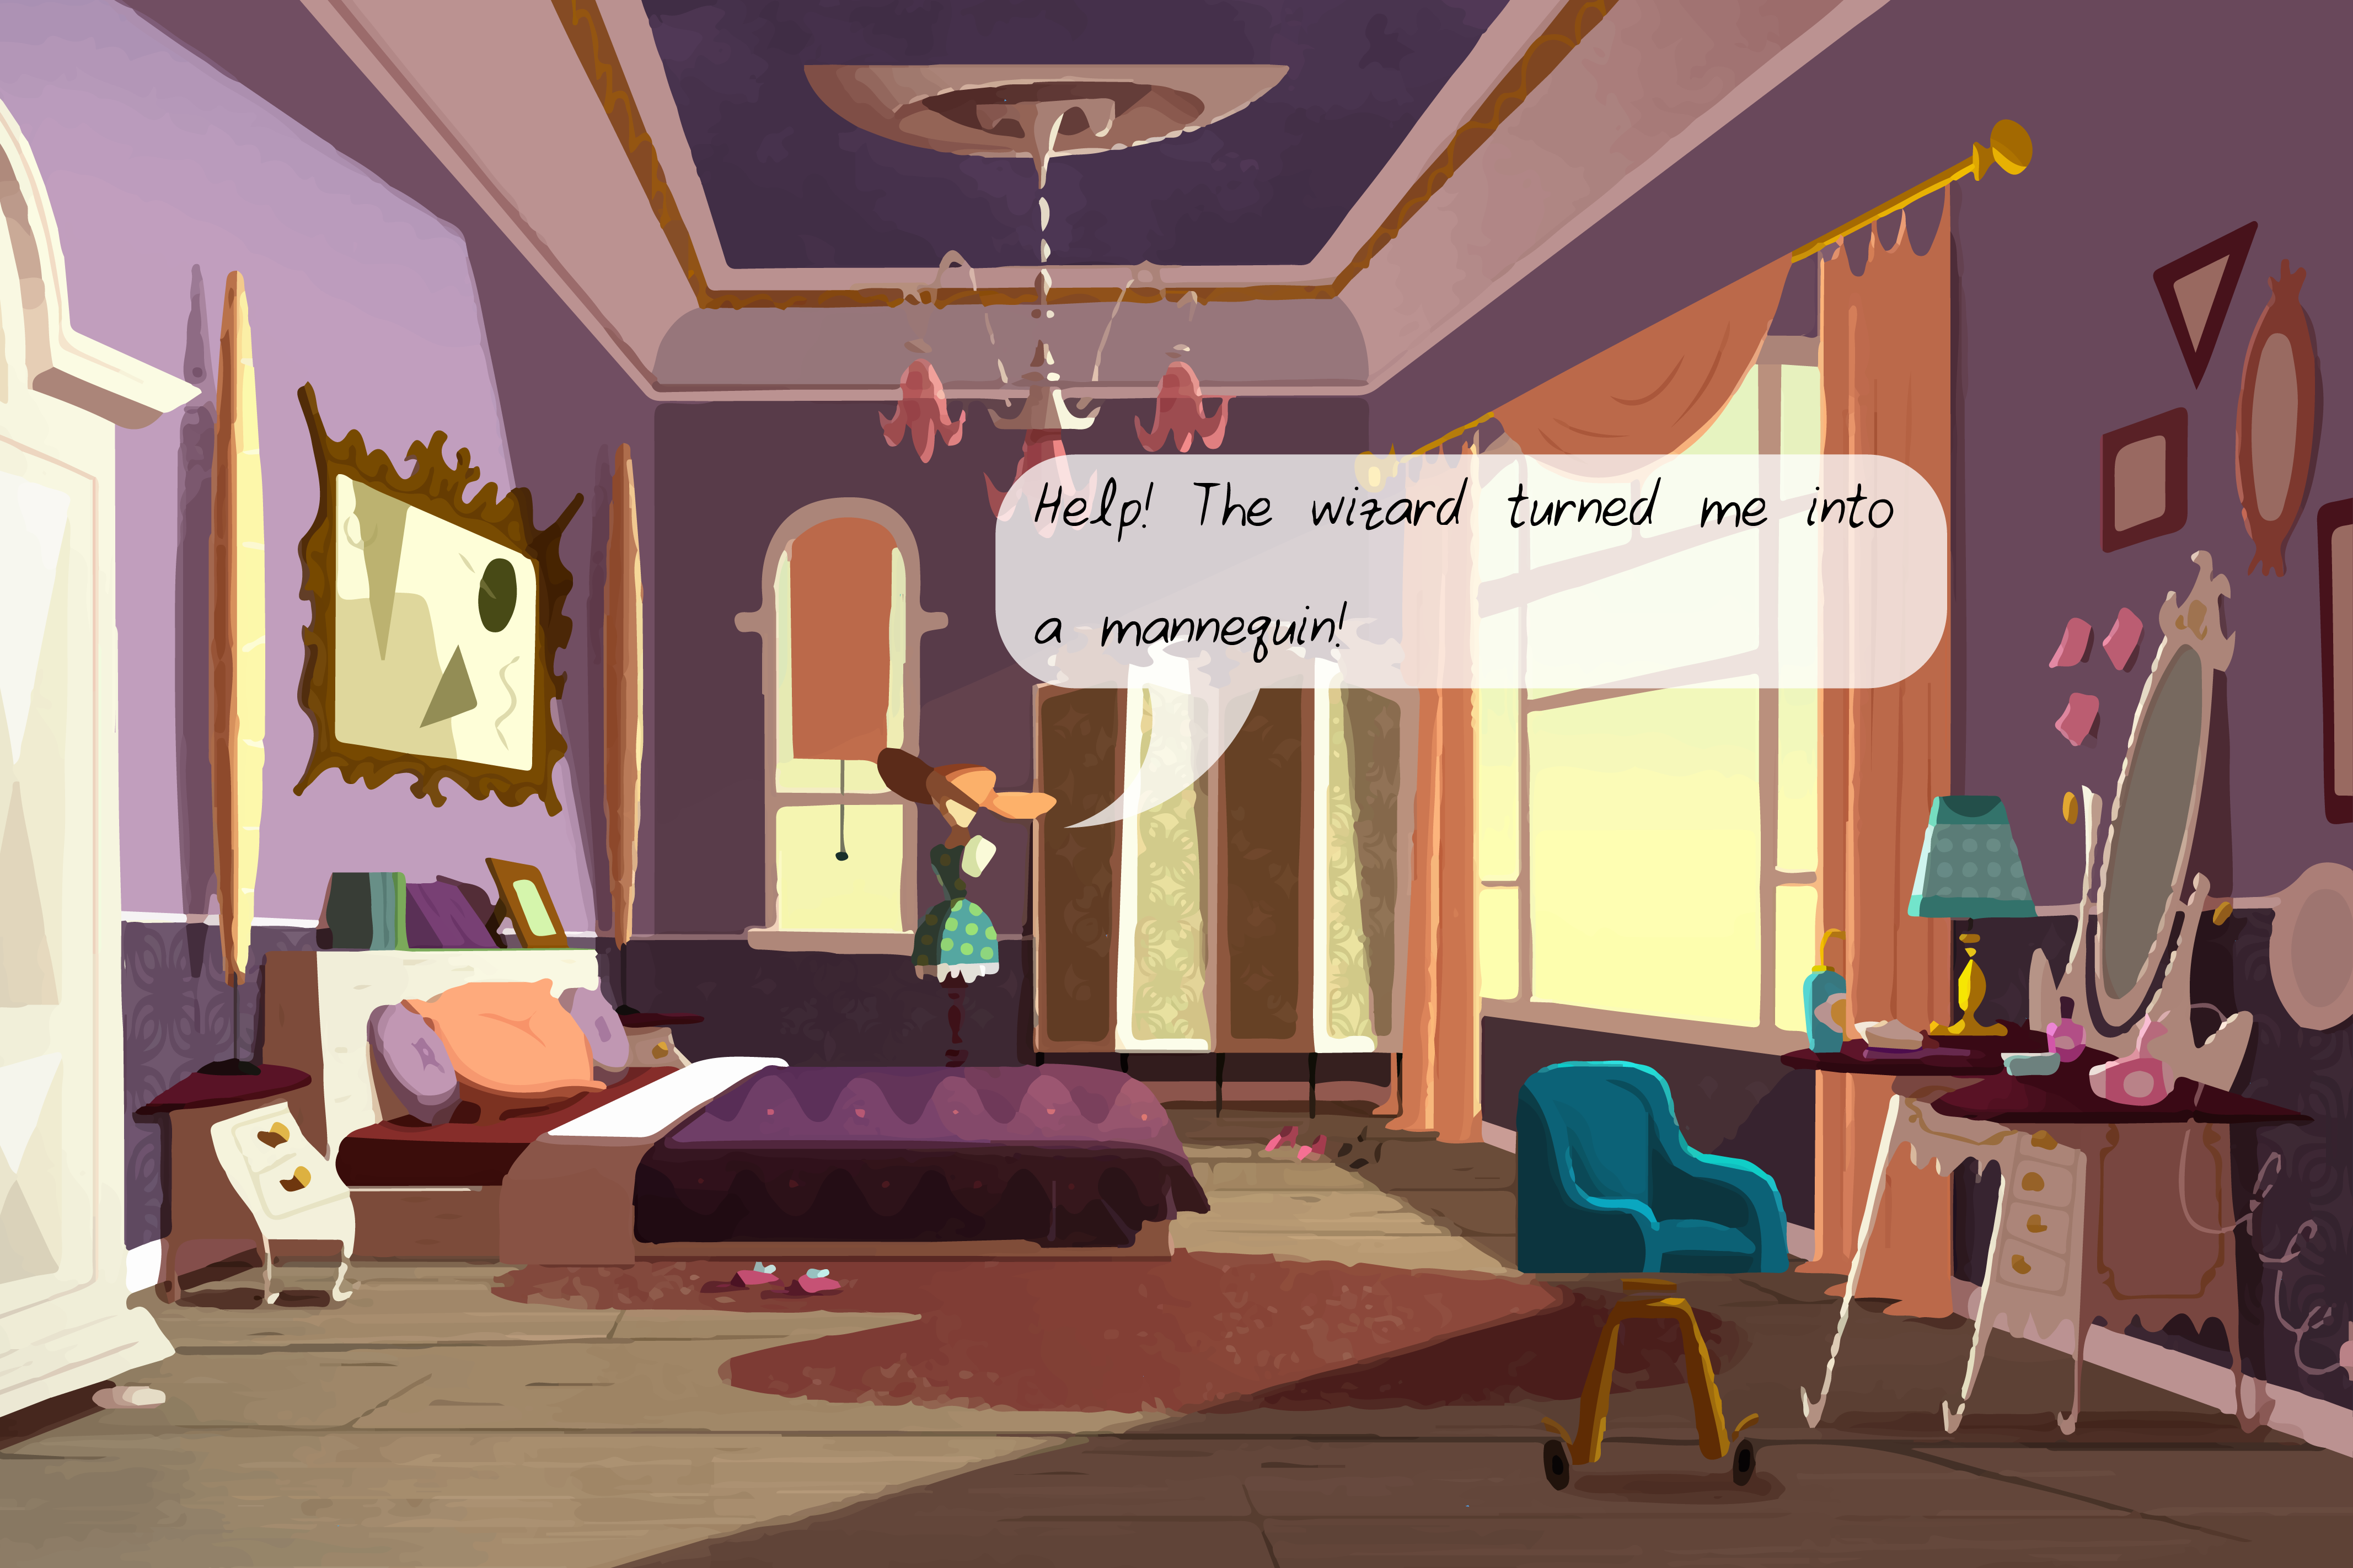
\includegraphics[width=2.3in]{figures/exp1/test-02.png} \\ 
% 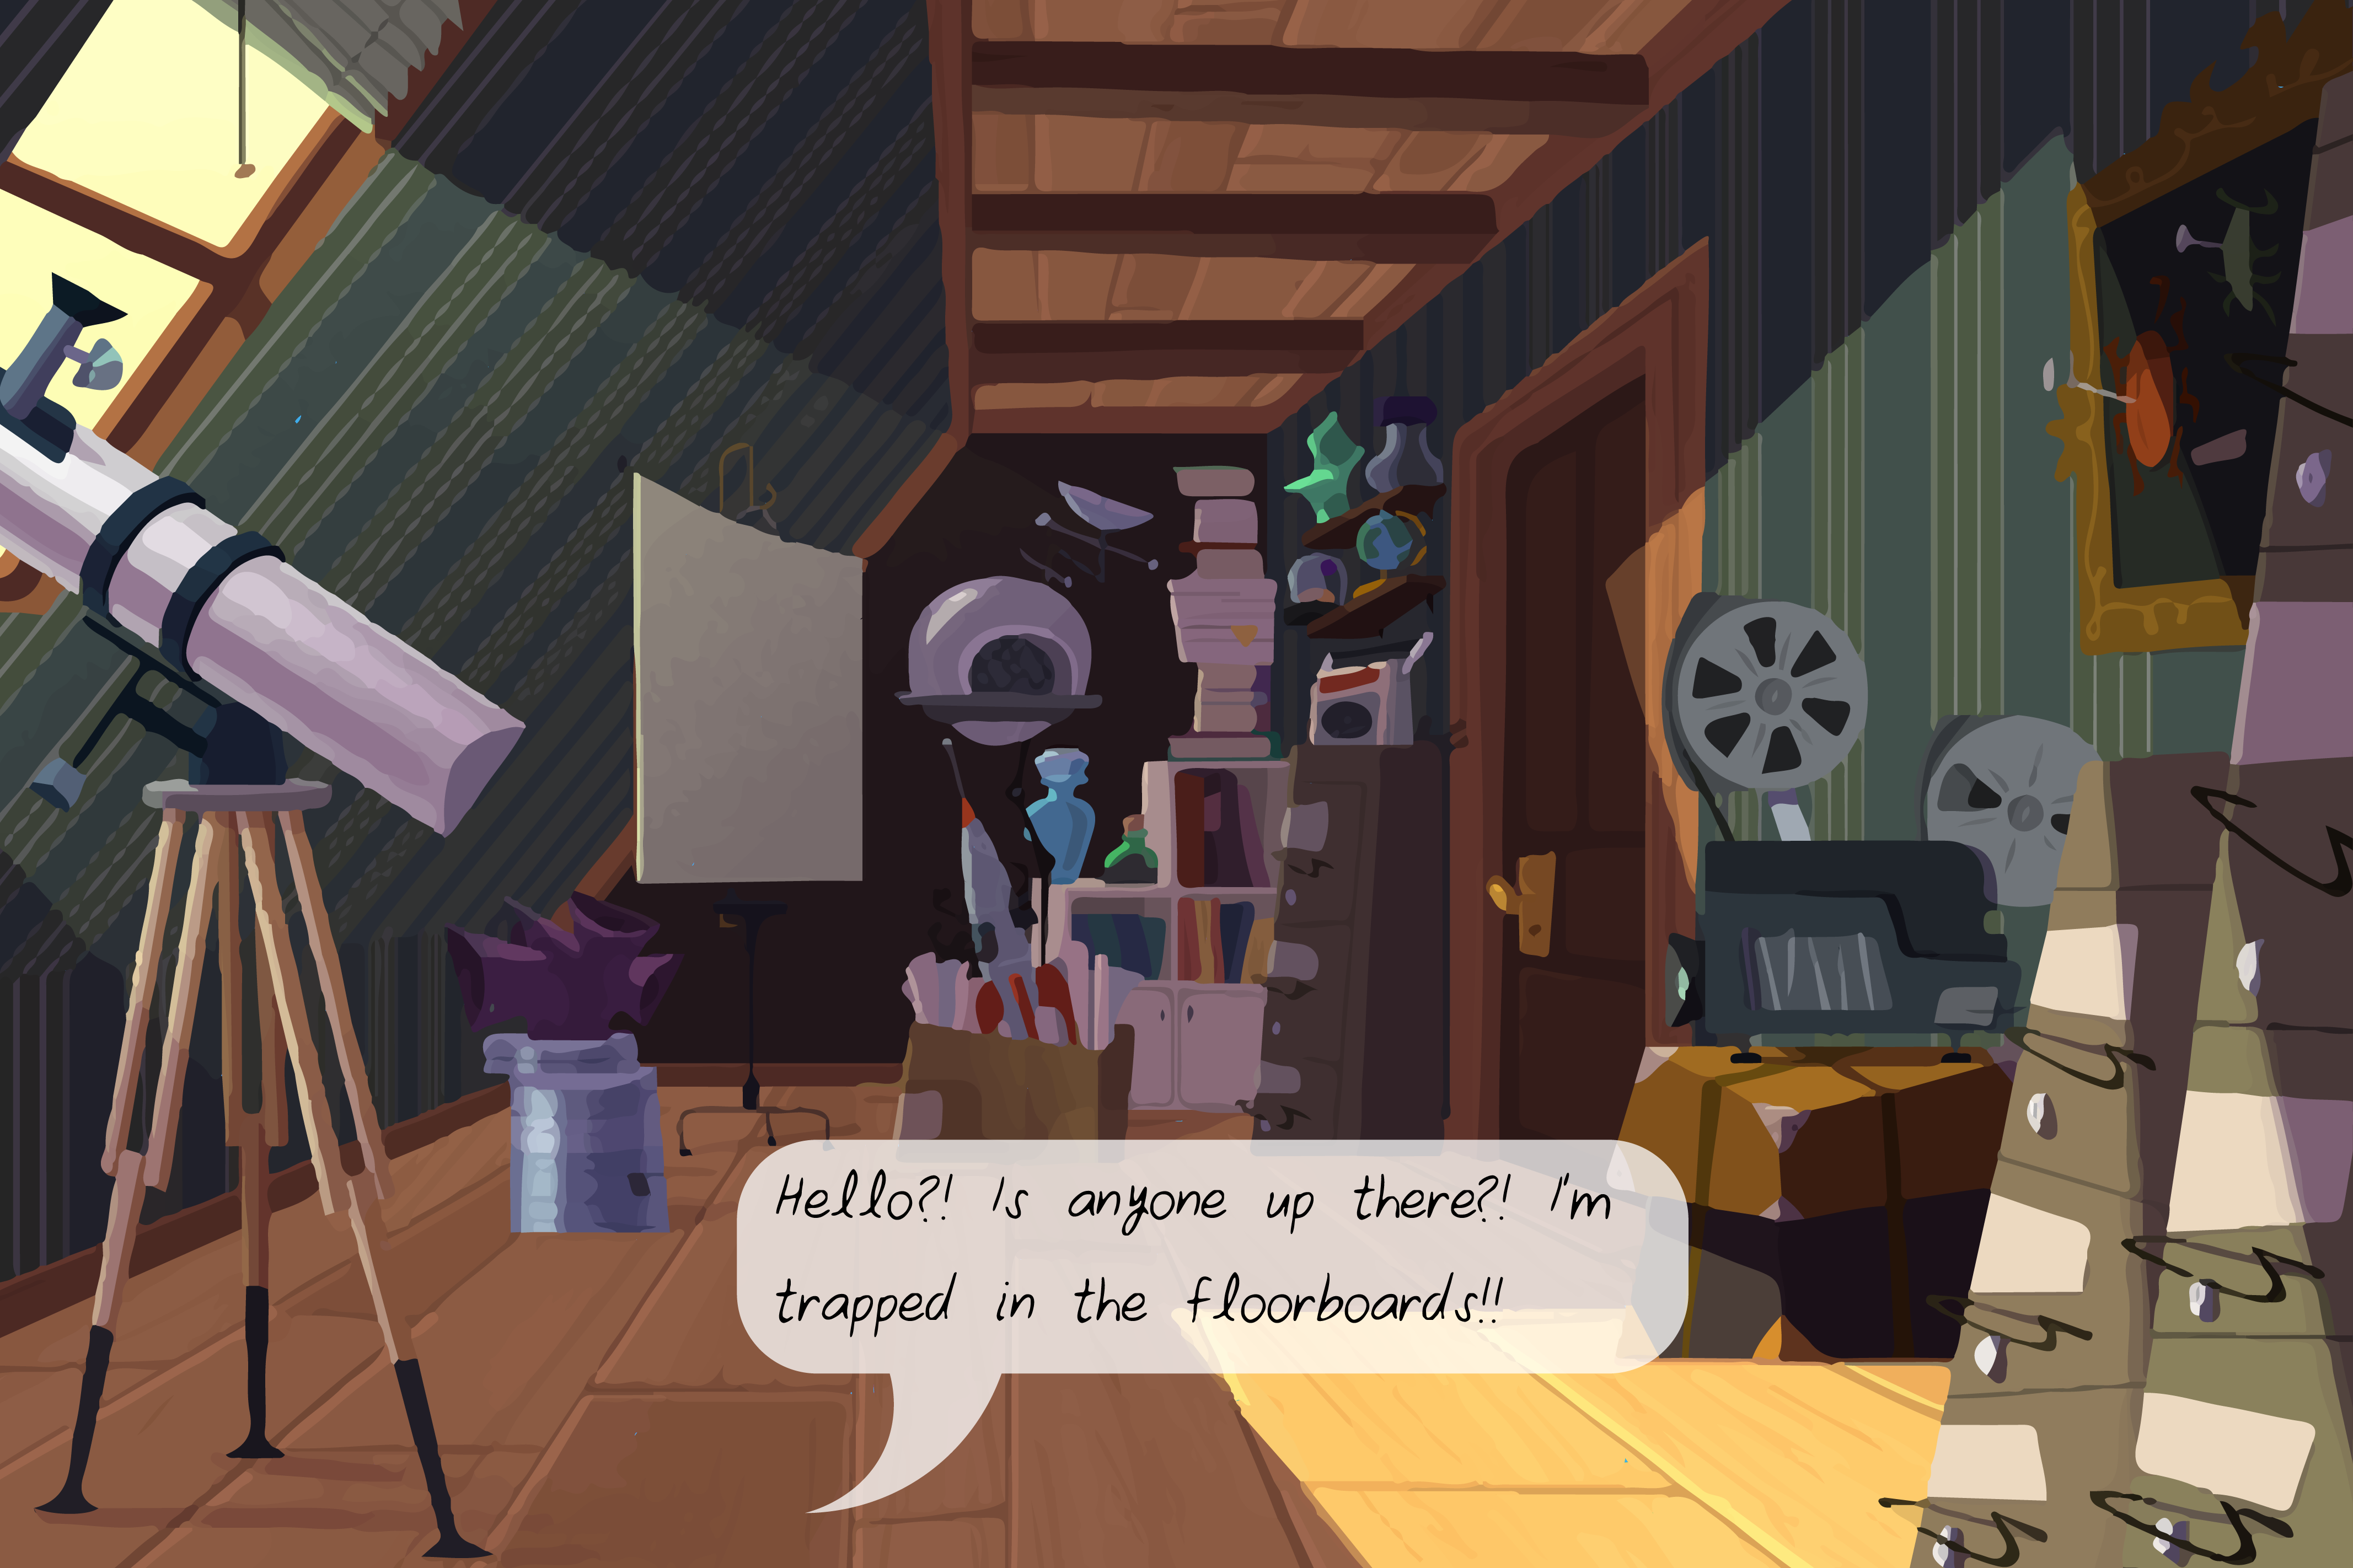
\includegraphics[width=2.3in]{figures/exp1/test-03.png} &
% 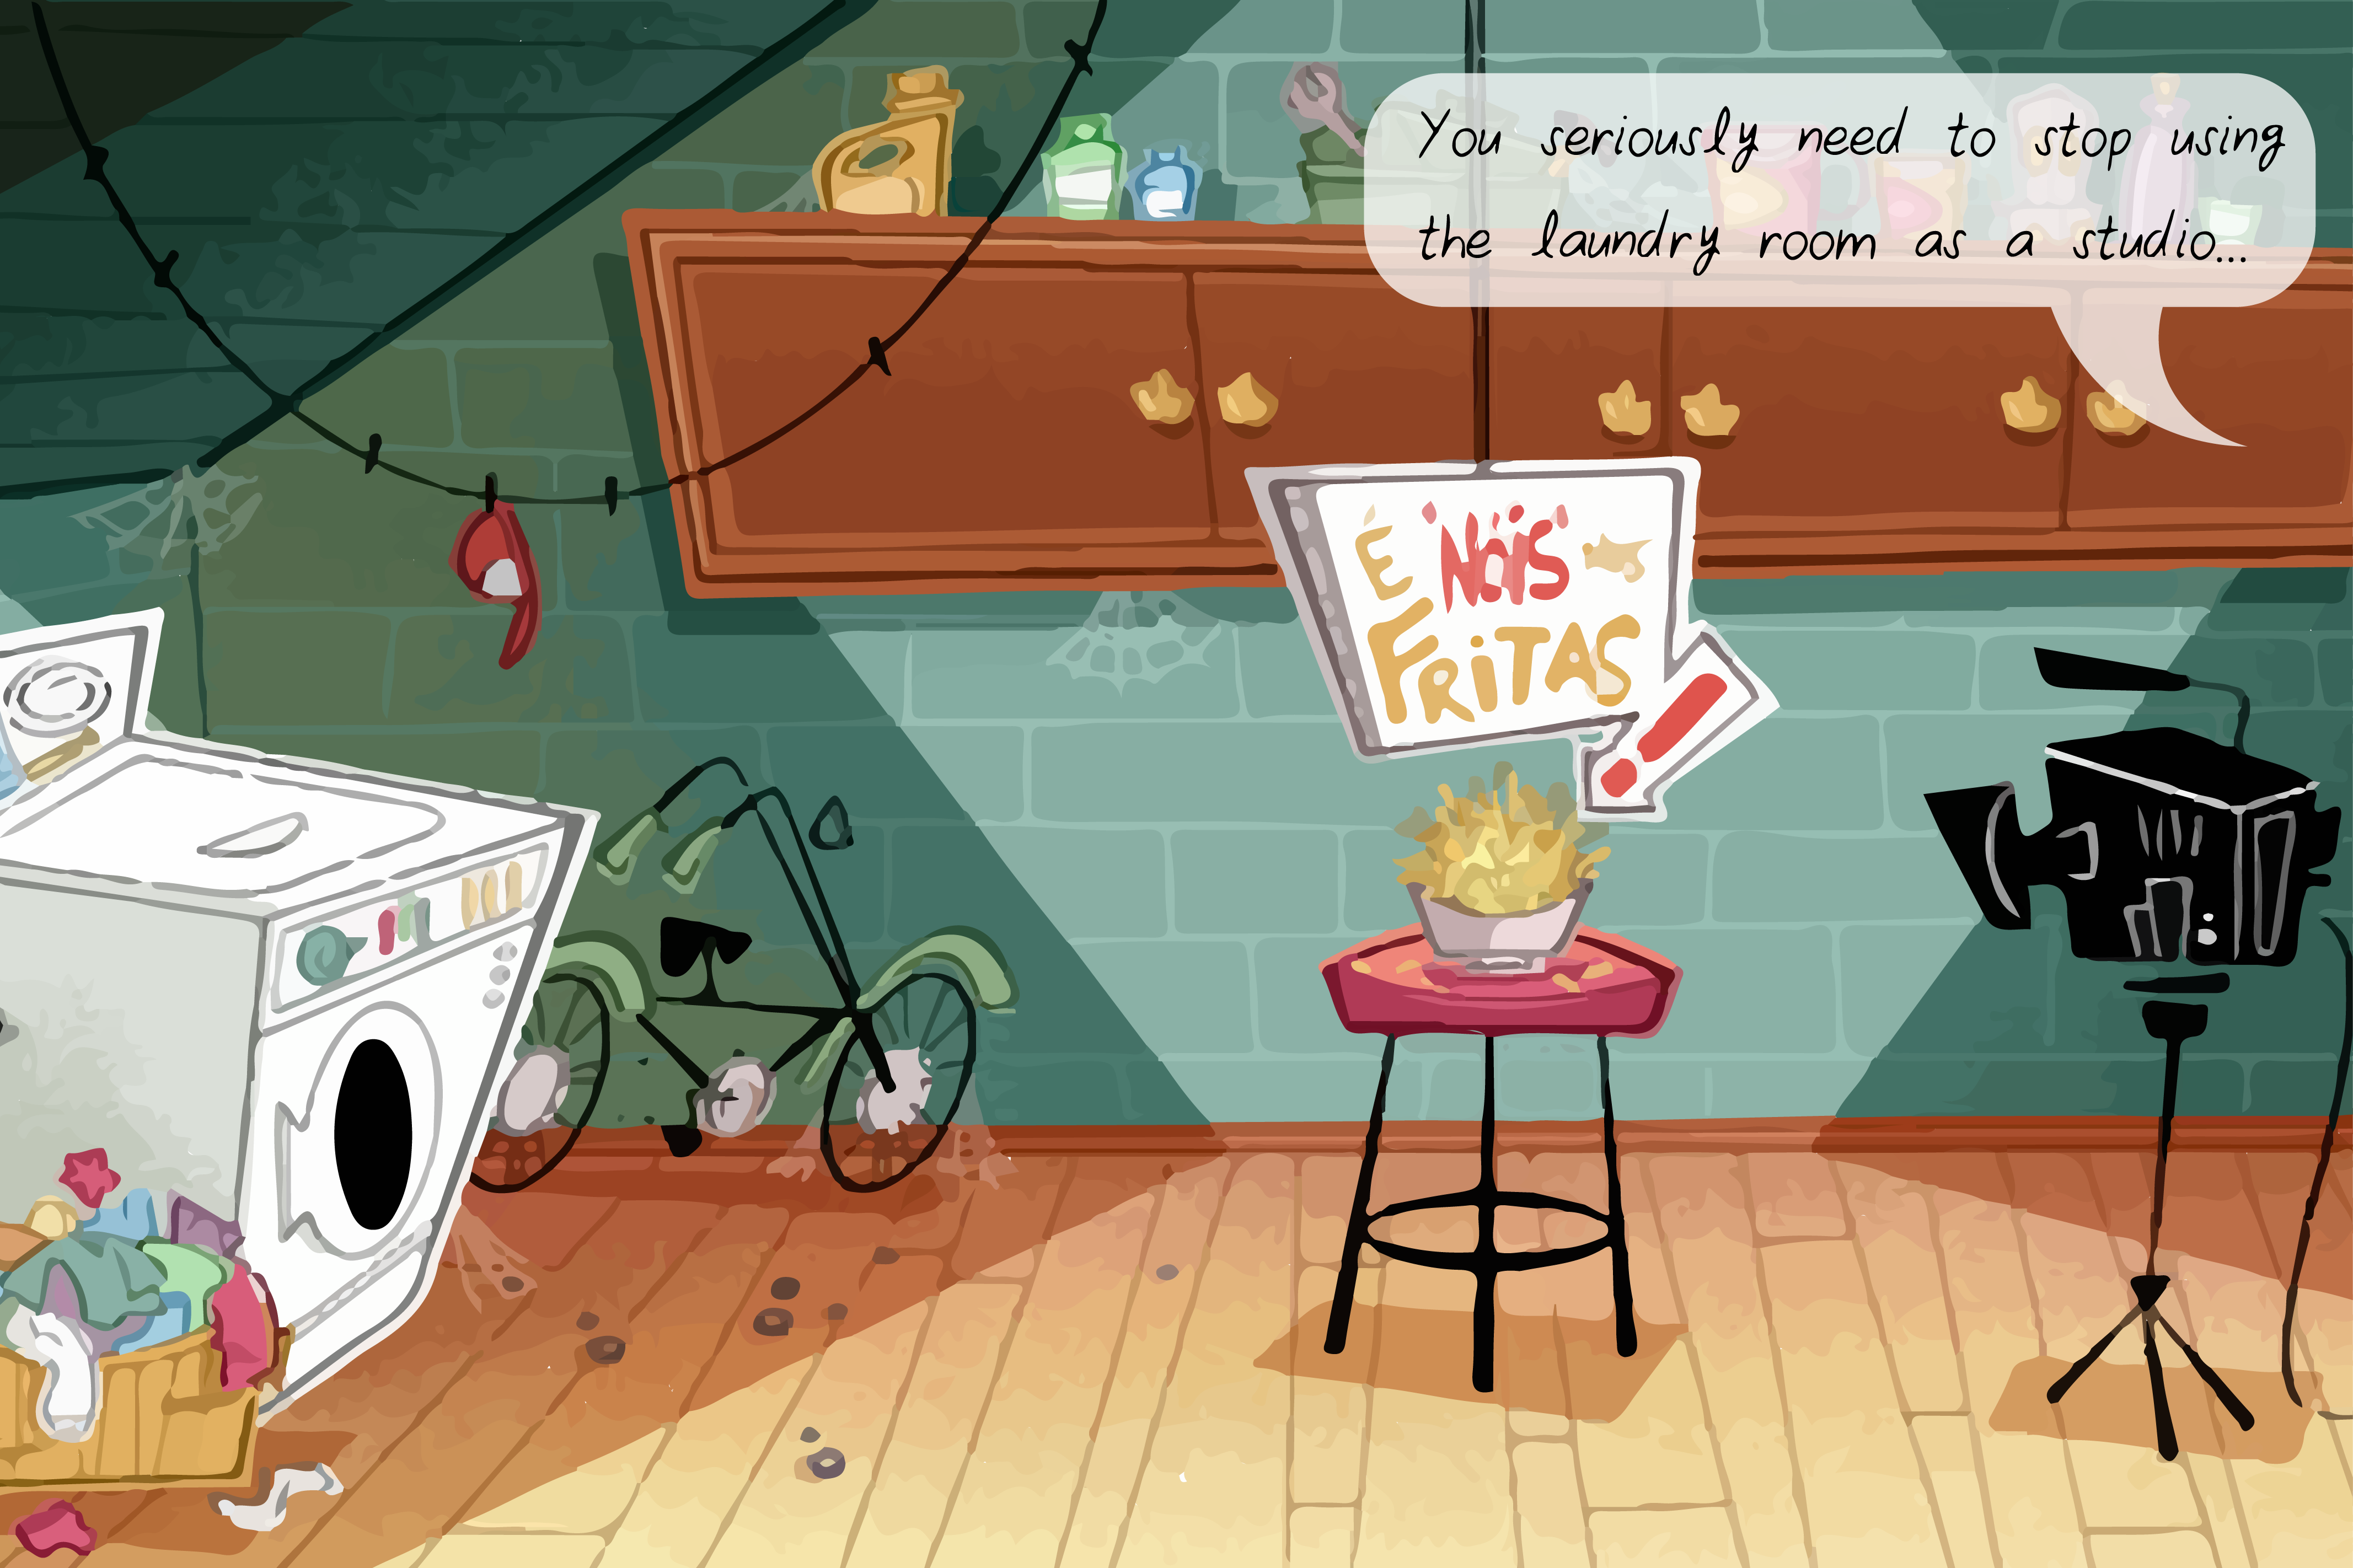
\includegraphics[width=2.3in]{figures/exp1/test-04.png} \\ 
% 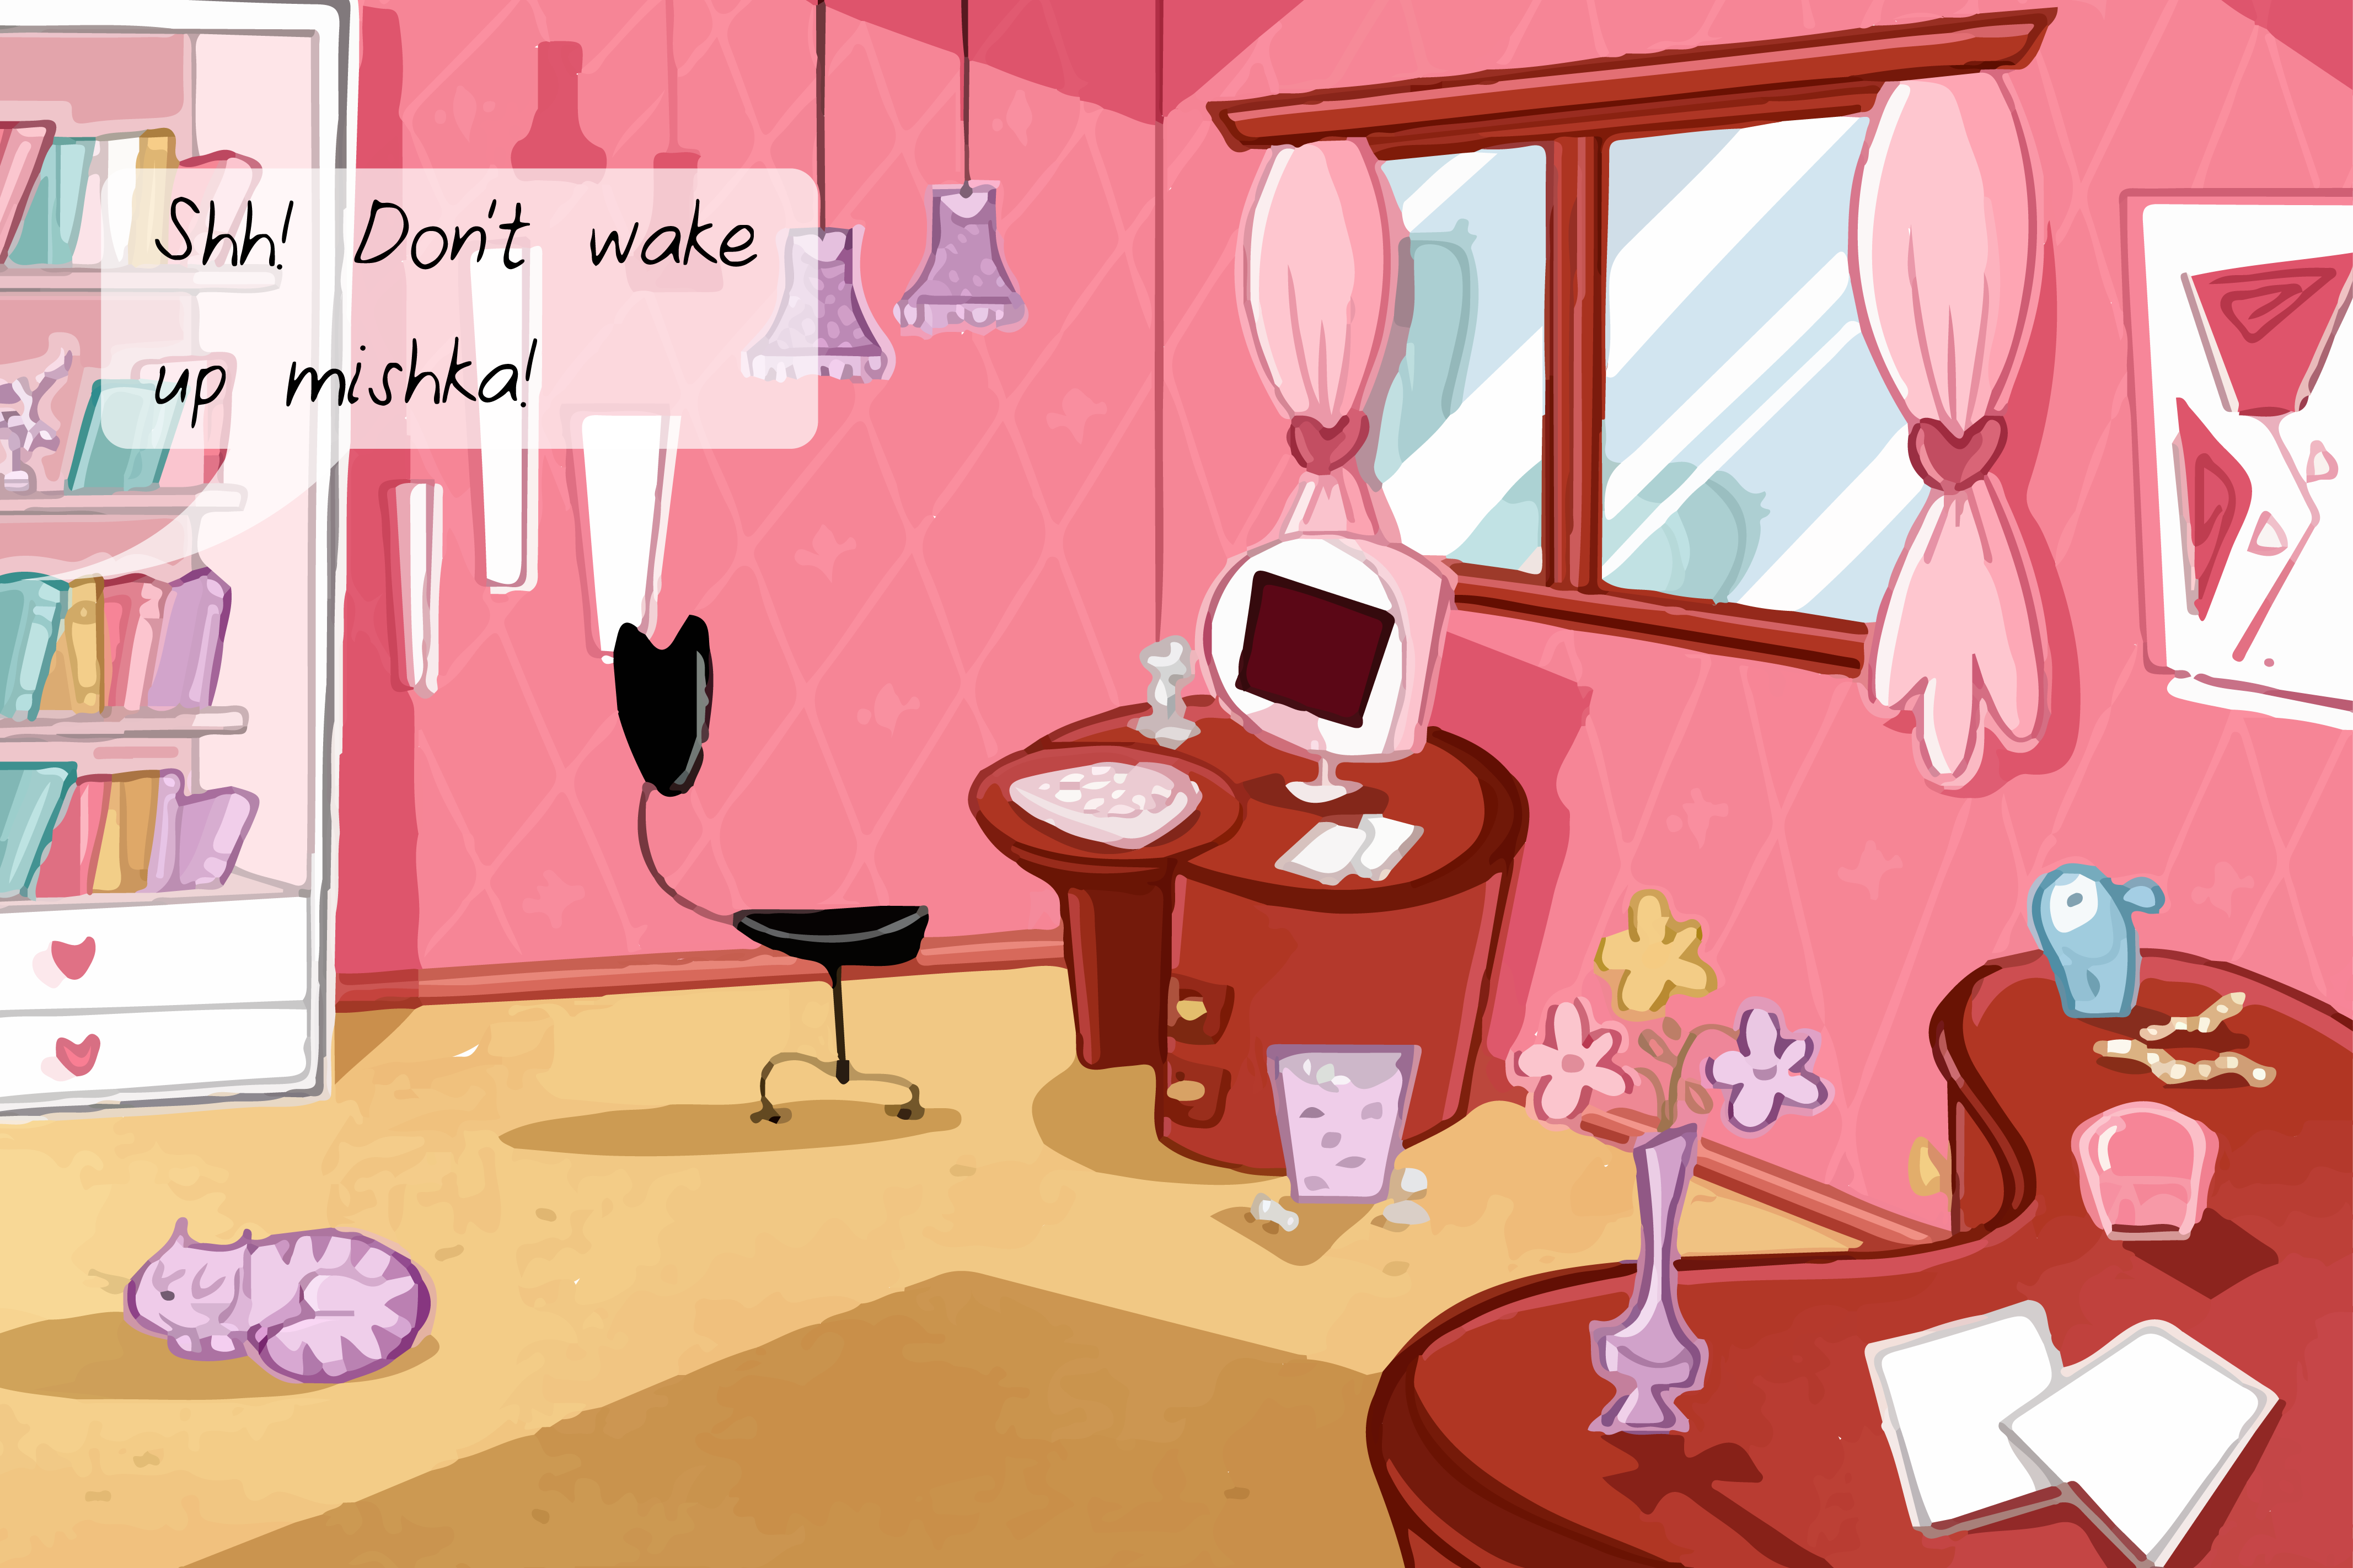
\includegraphics[width=2.3in]{figures/exp1/test-05.png} &
% 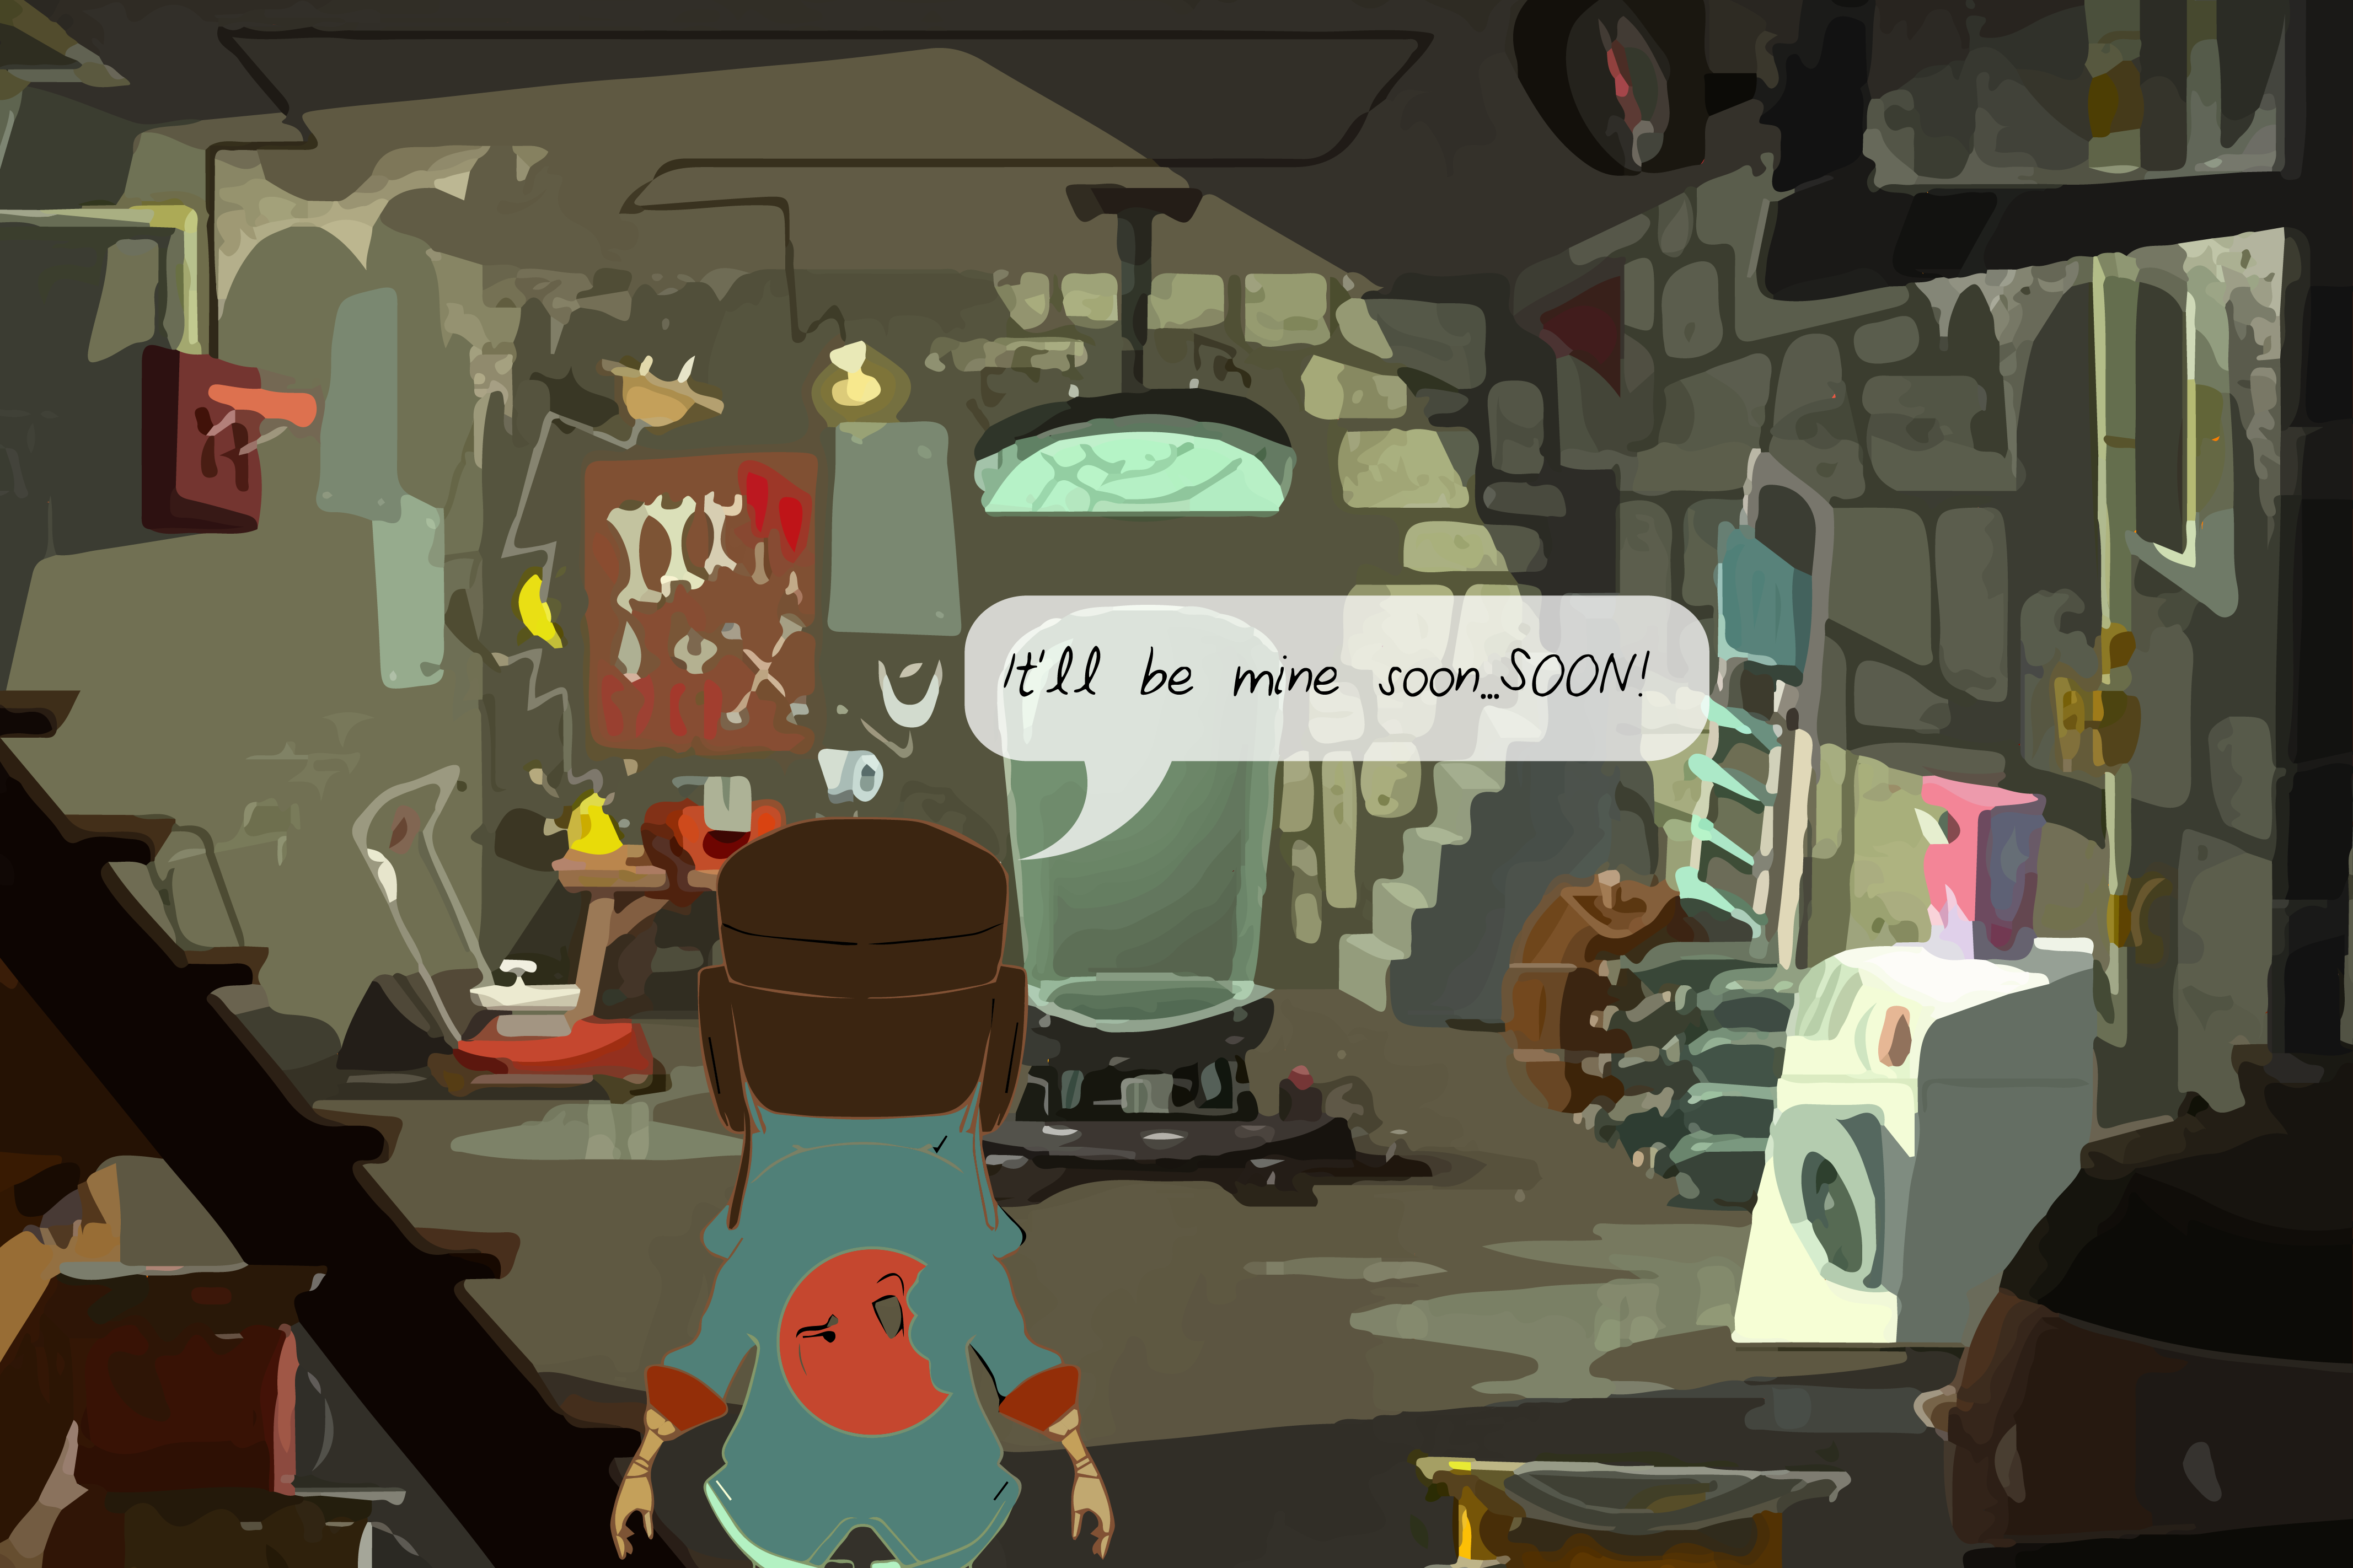
\includegraphics[width=2.3in]{figures/exp1/test-06.png} \\ 
% 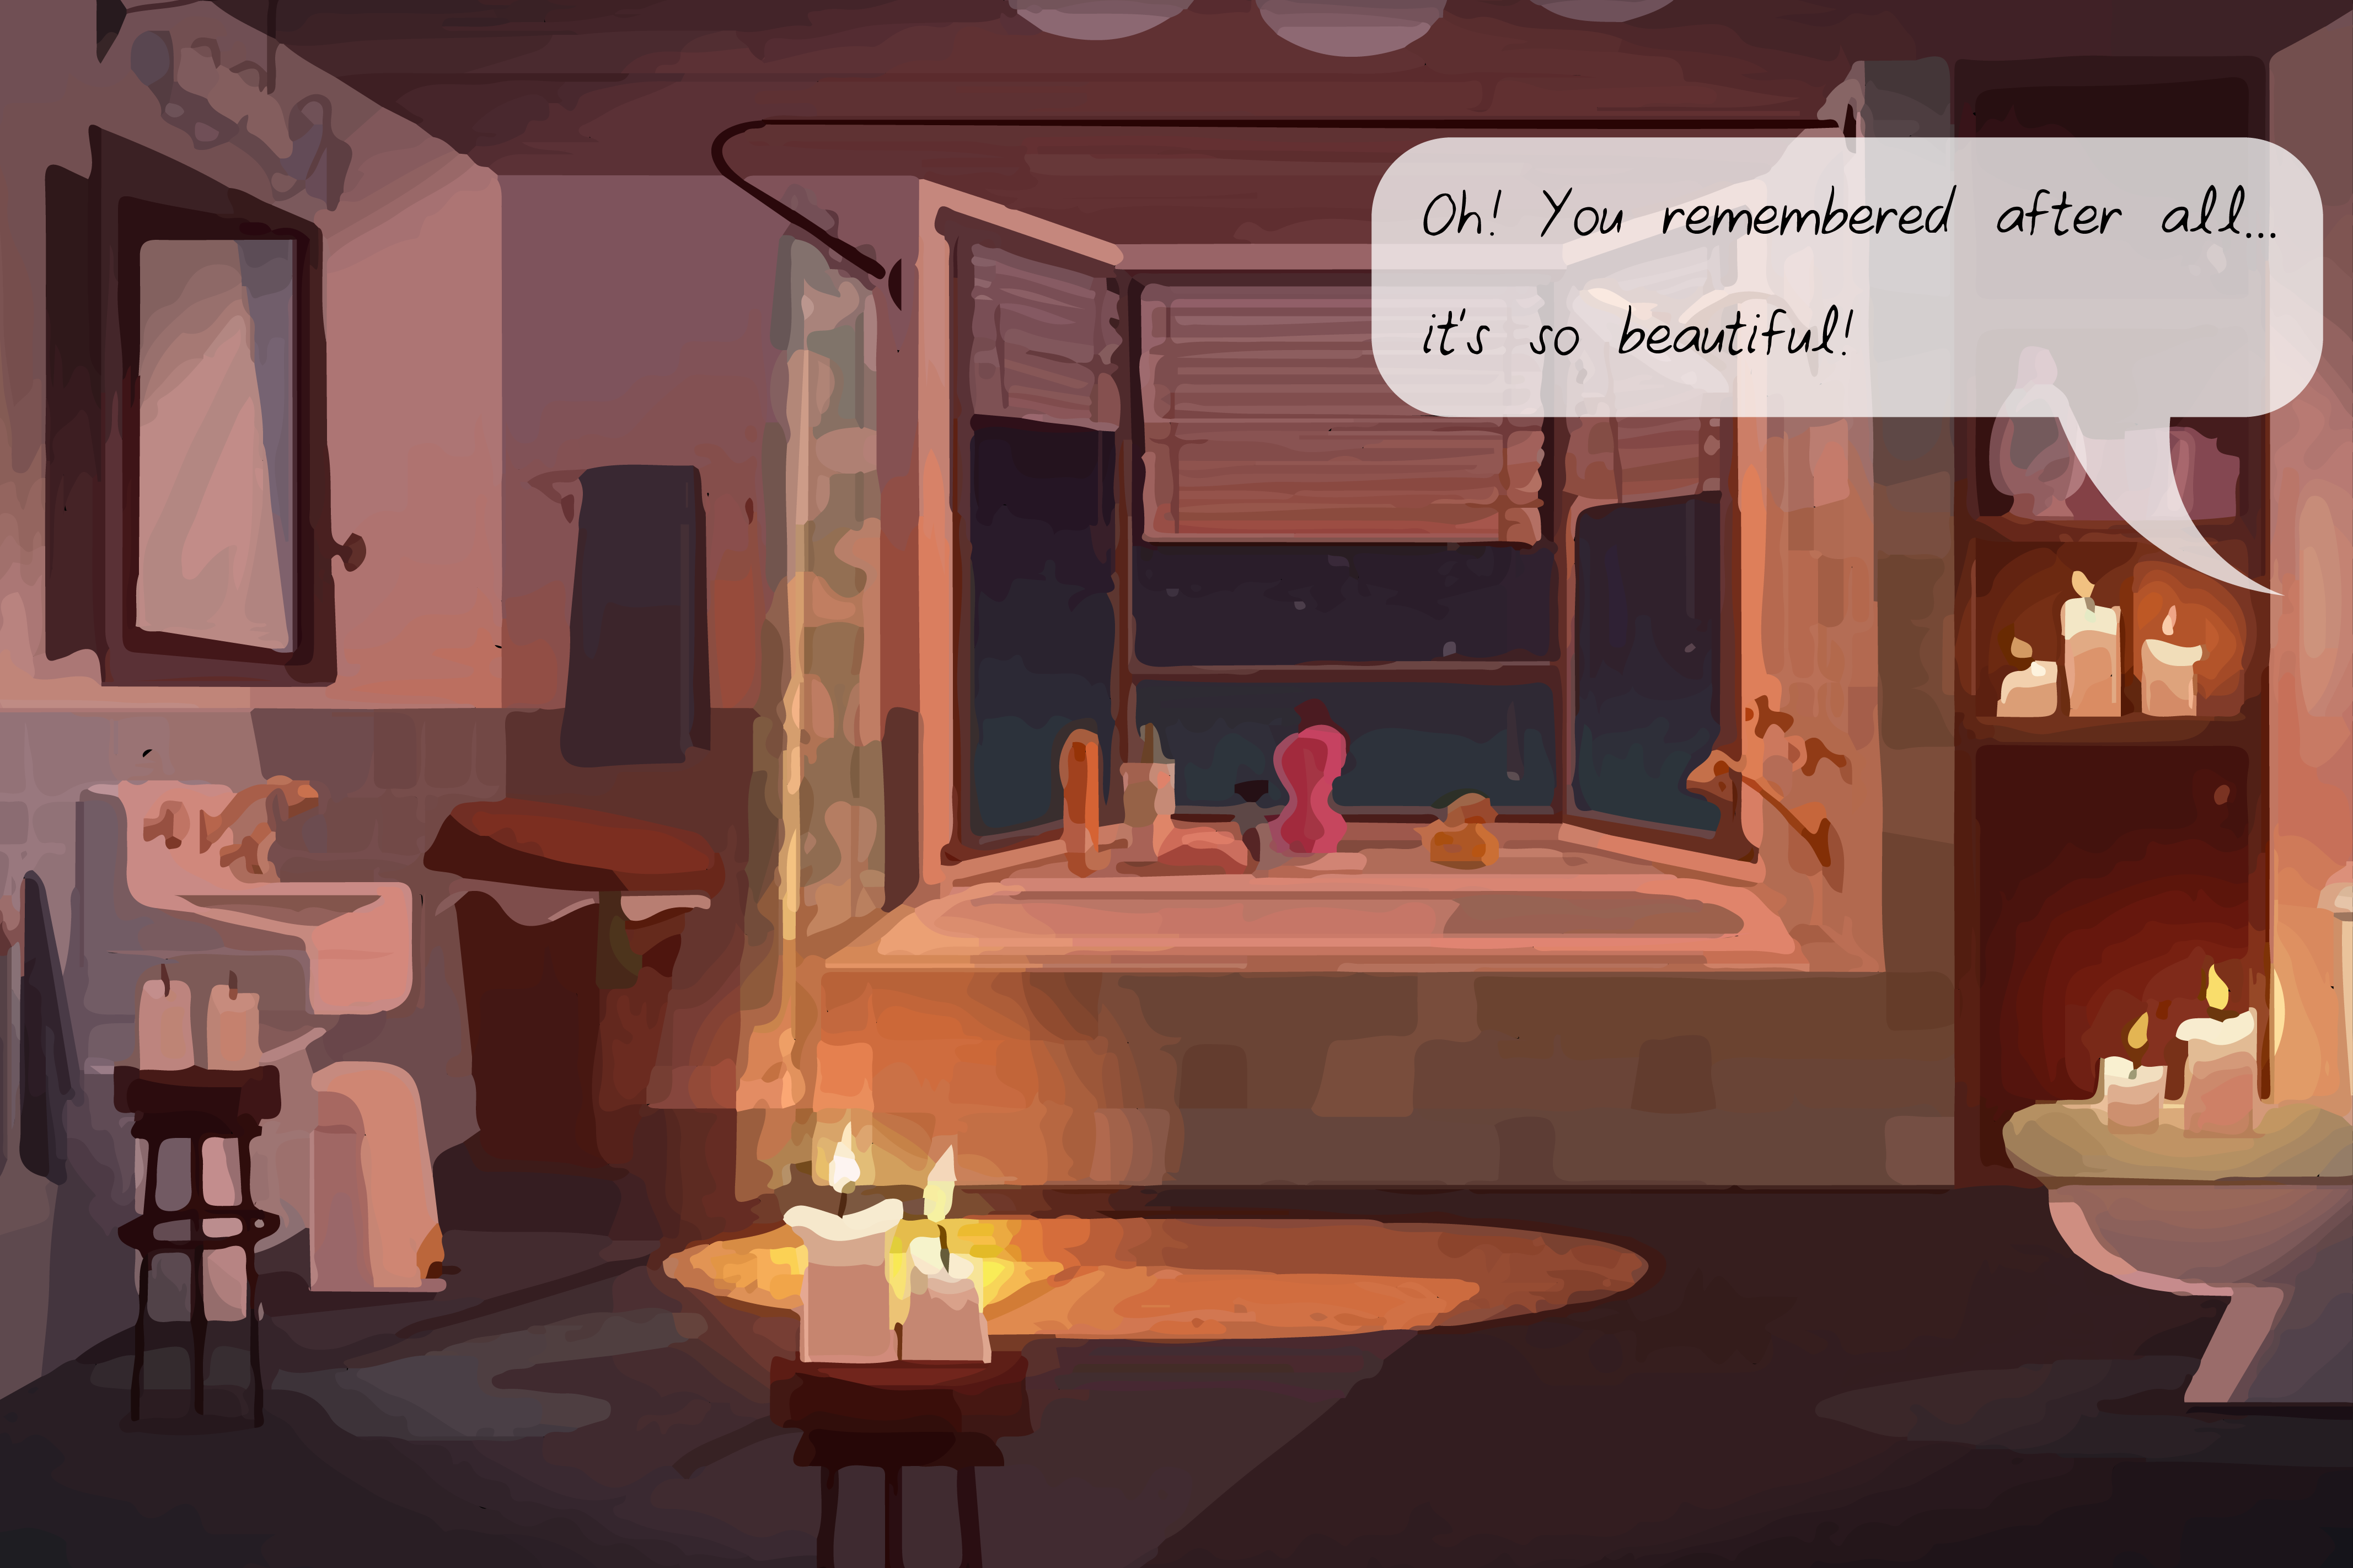
\includegraphics[width=2.3in]{figures/exp1/test-07.png} &
% 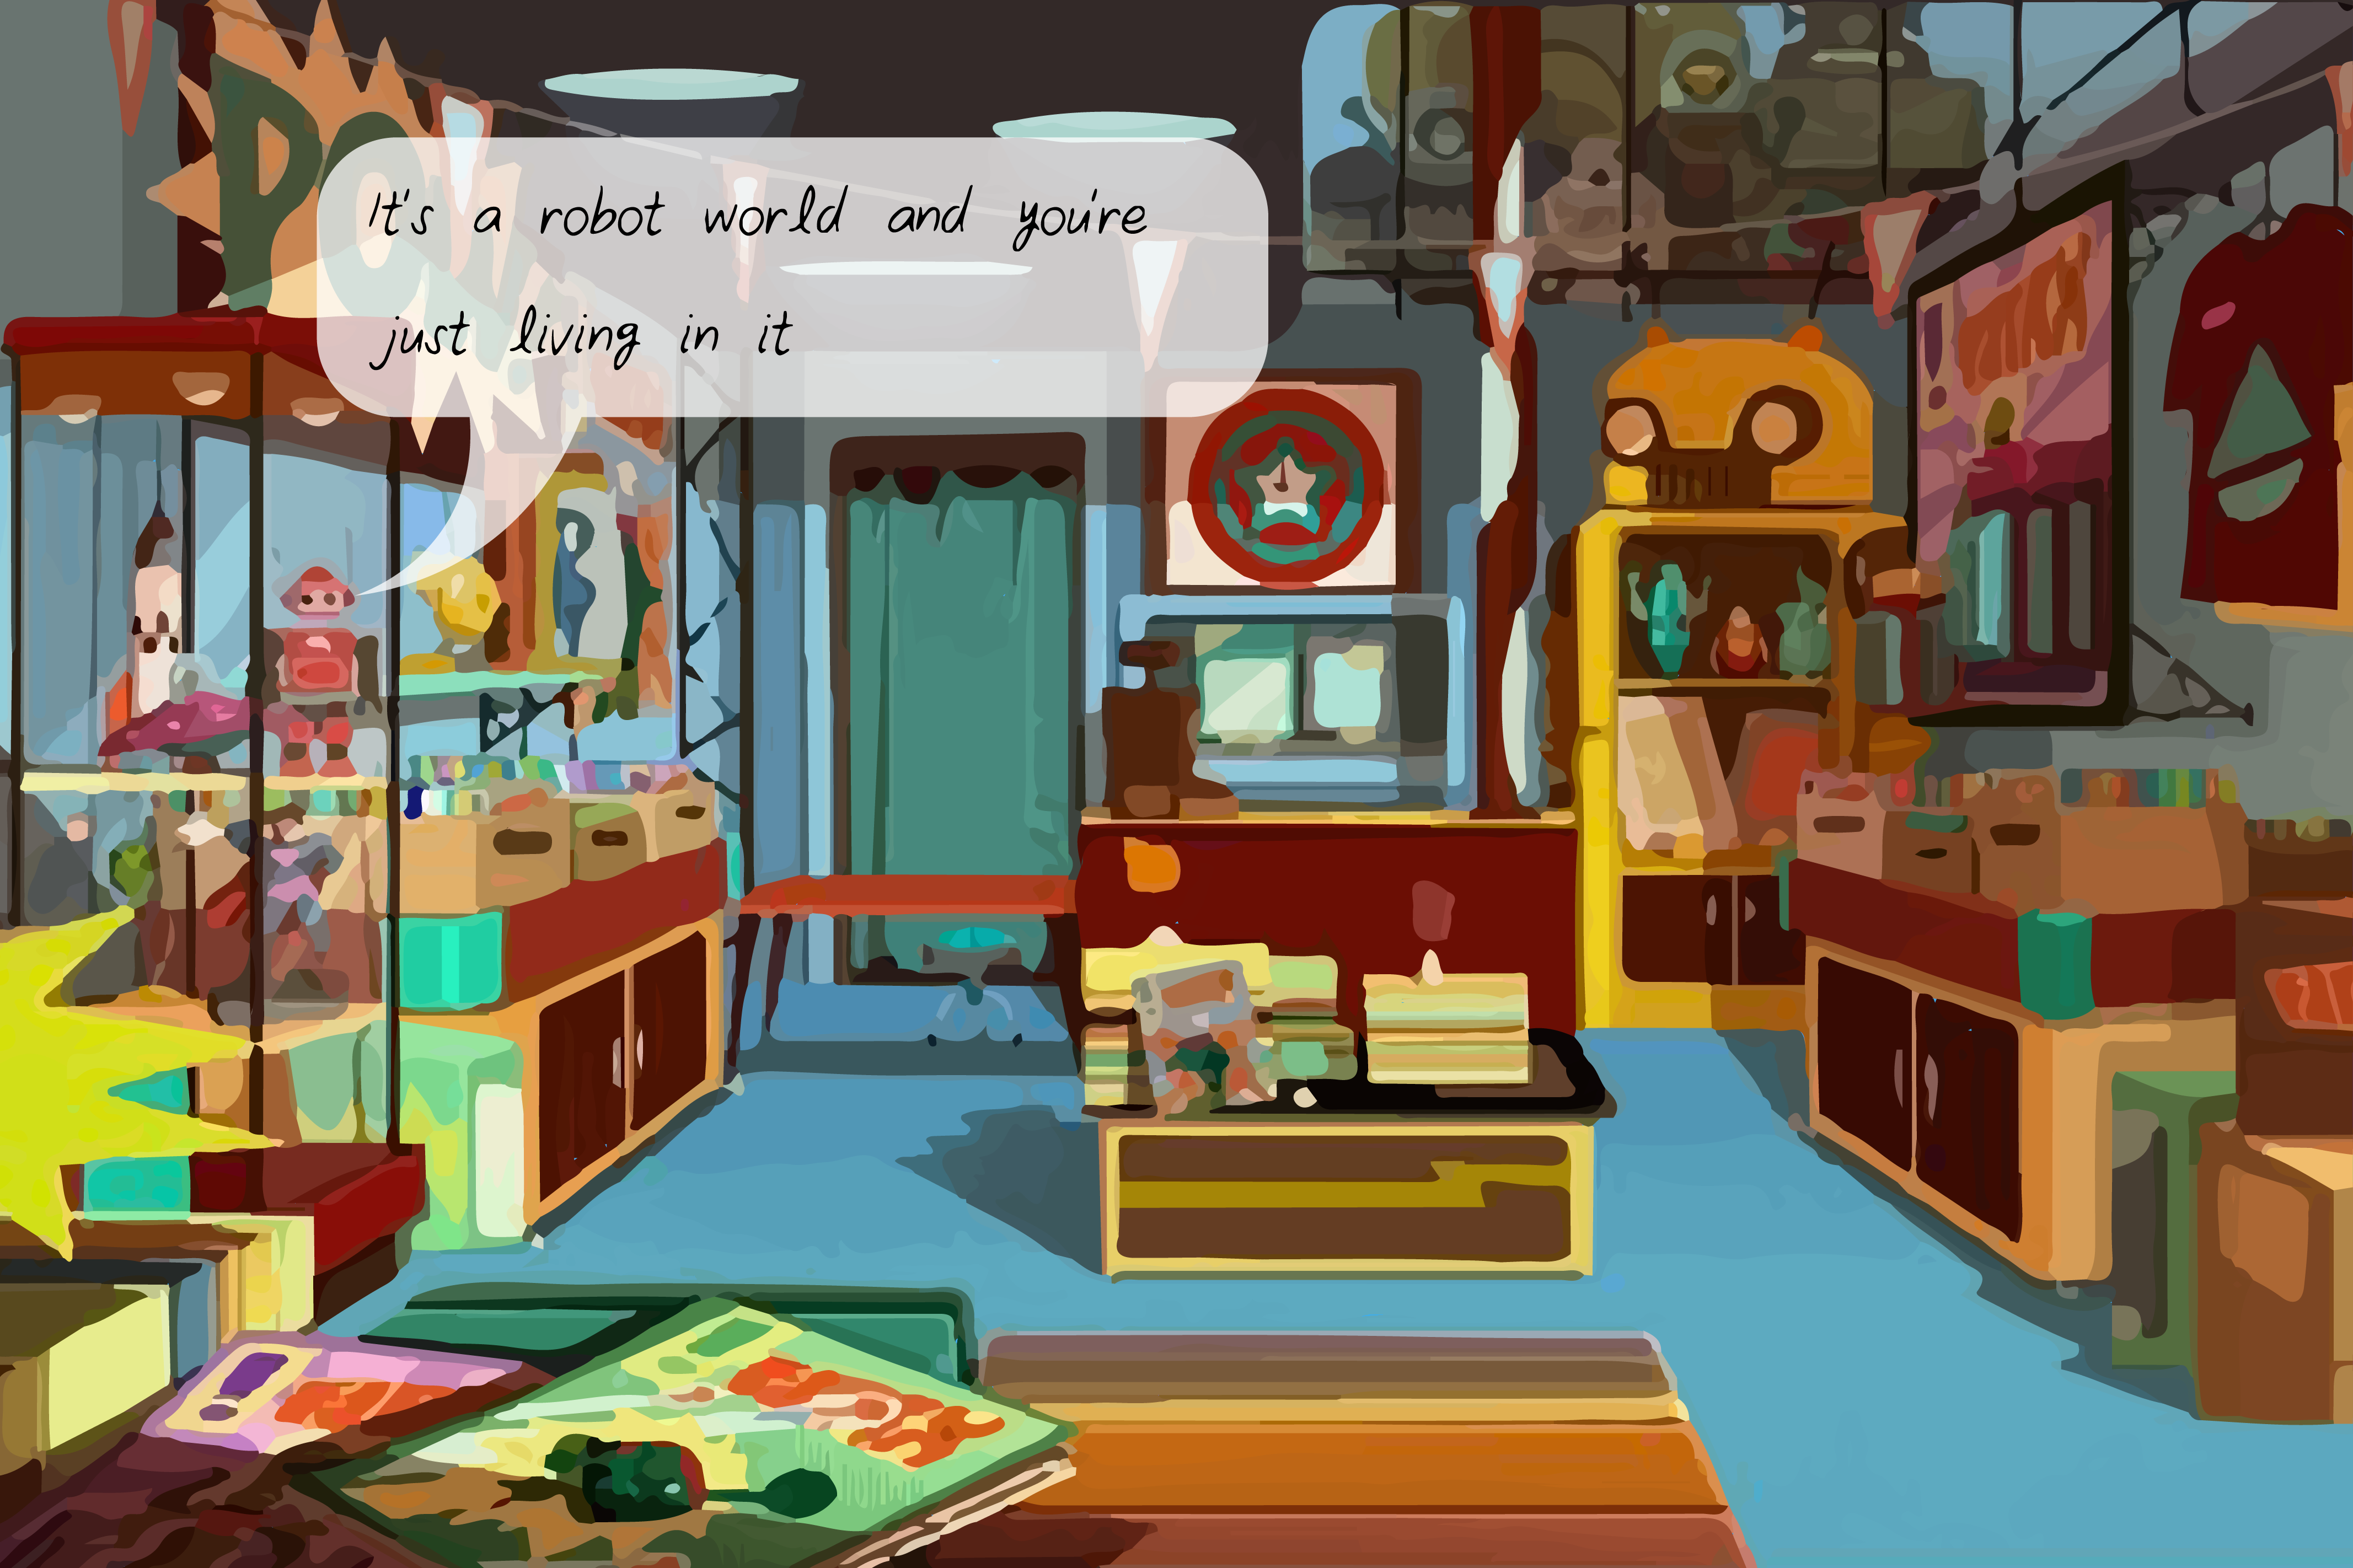
\includegraphics[width=2.3in]{figures/exp1/test-08.png} \\ 
% 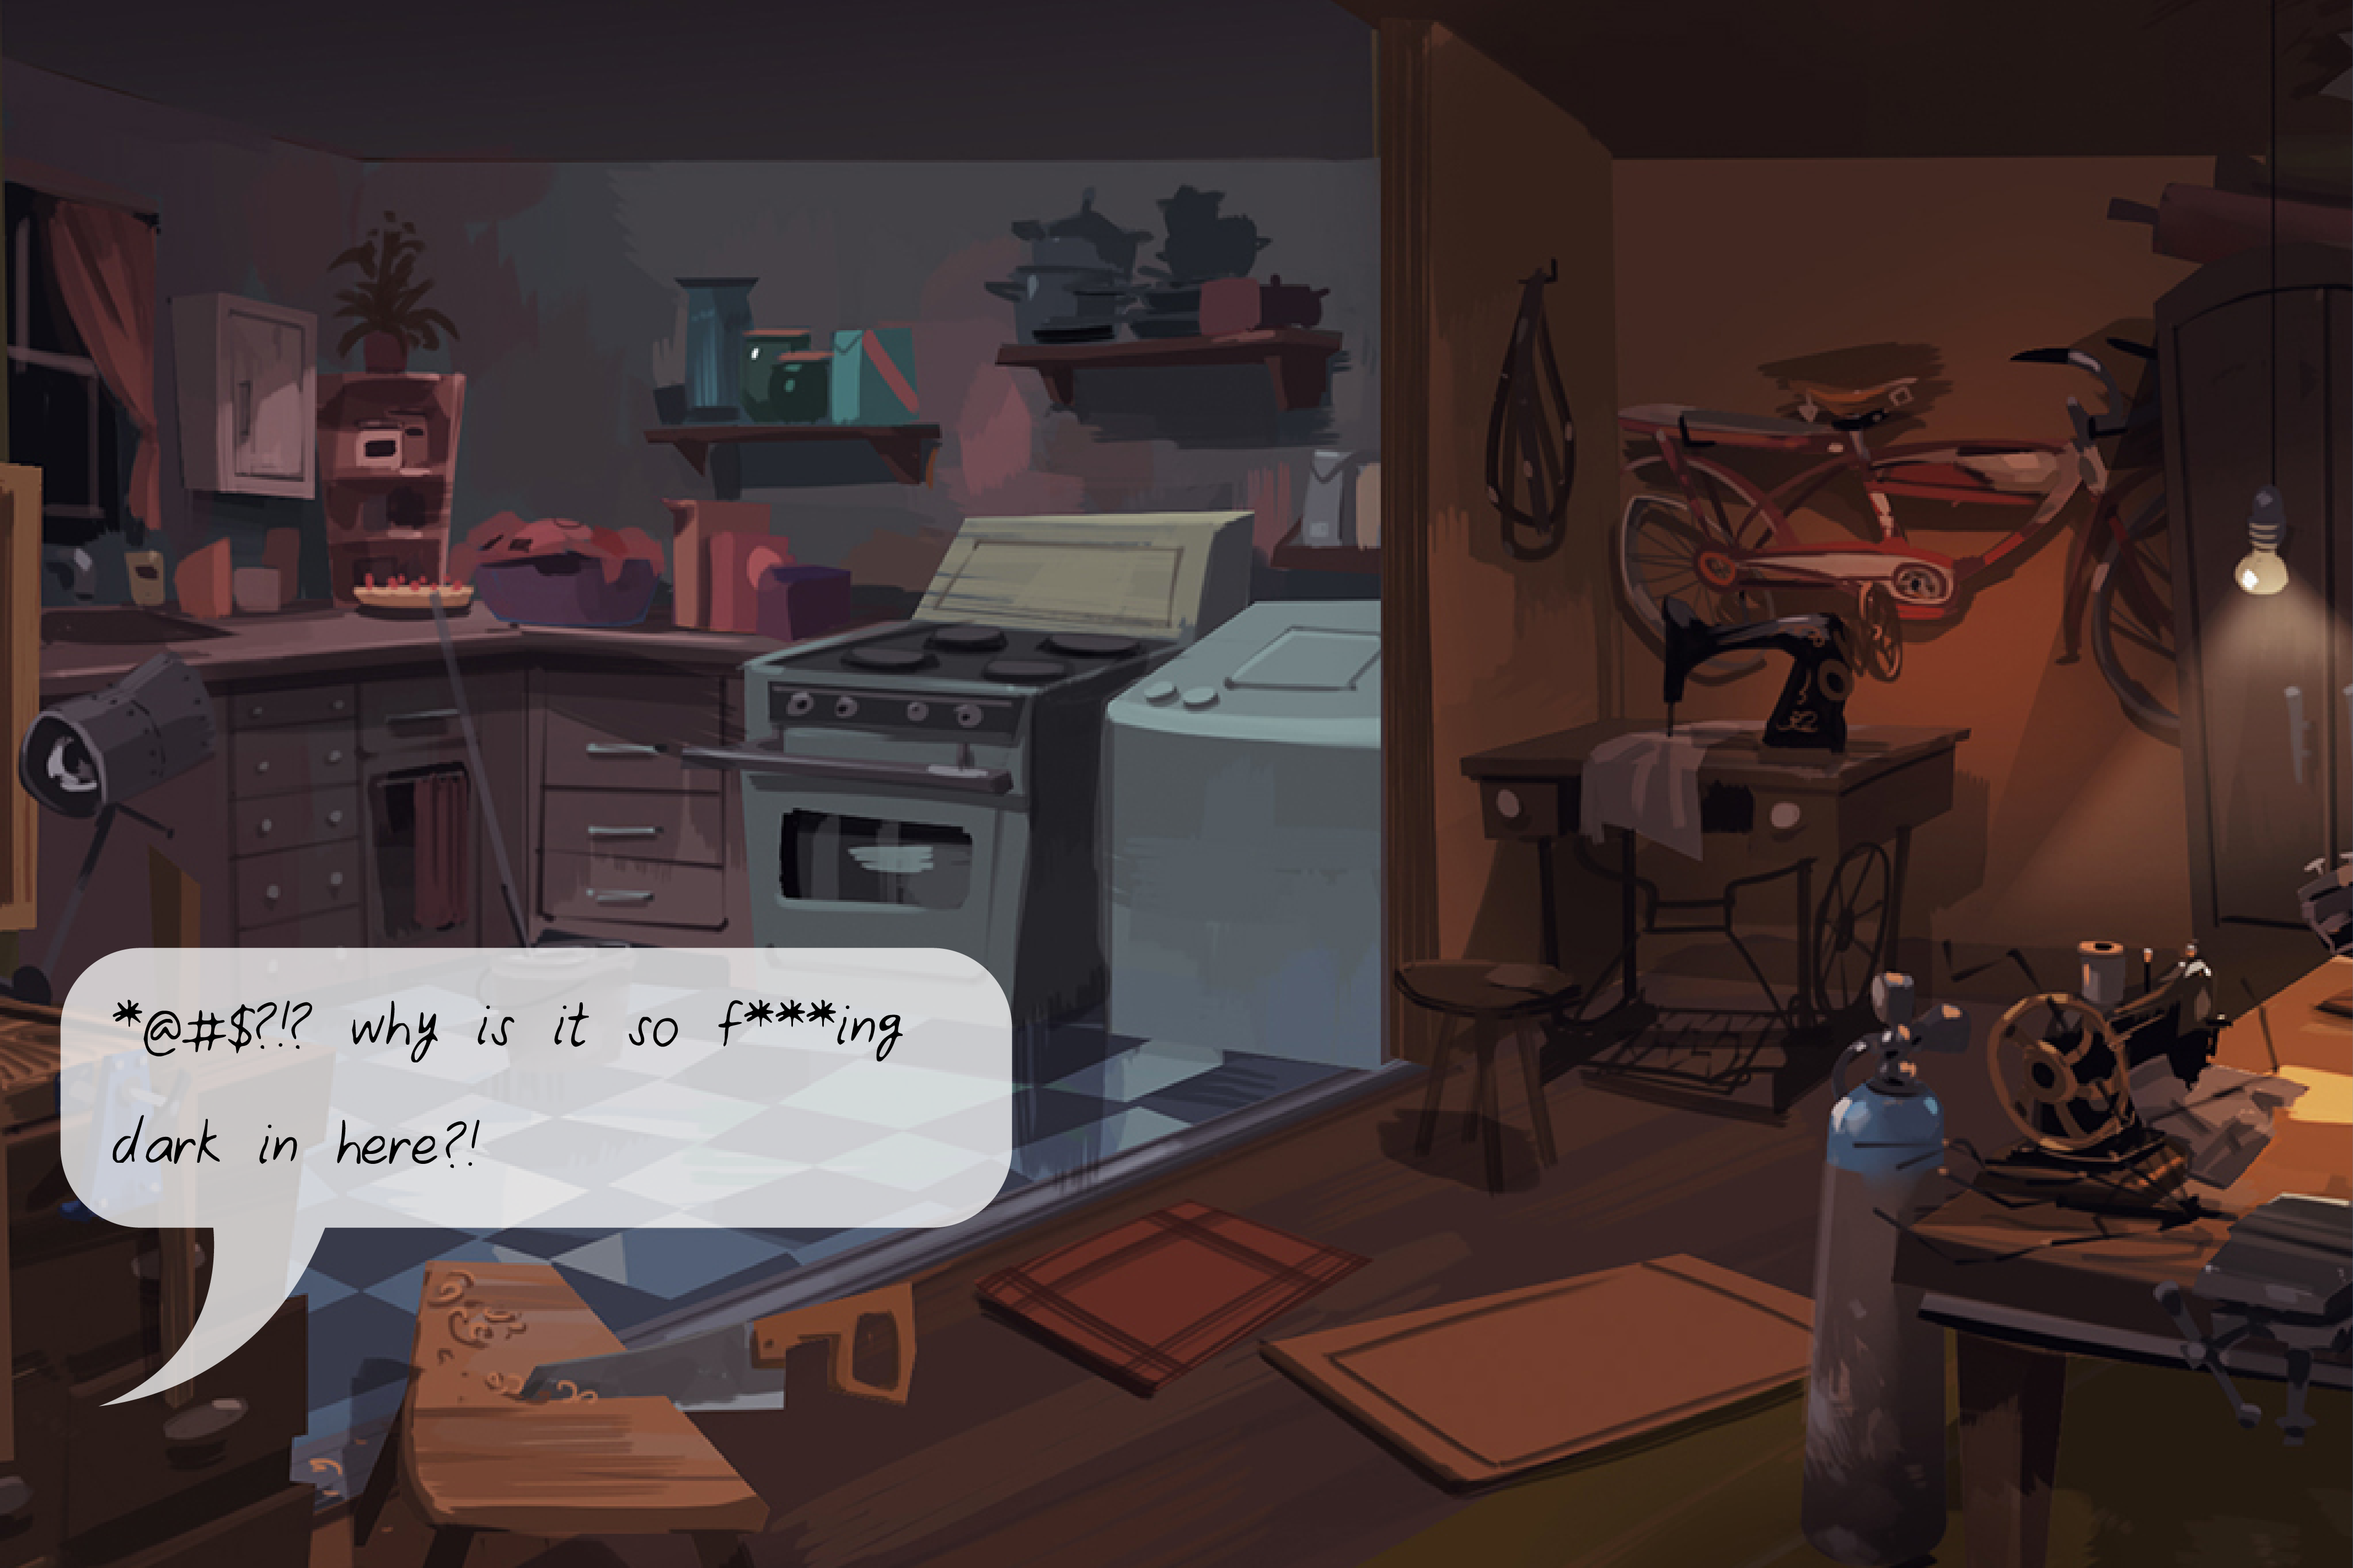
\includegraphics[width=2.3in]{figures/exp1/test-09.png} &
% 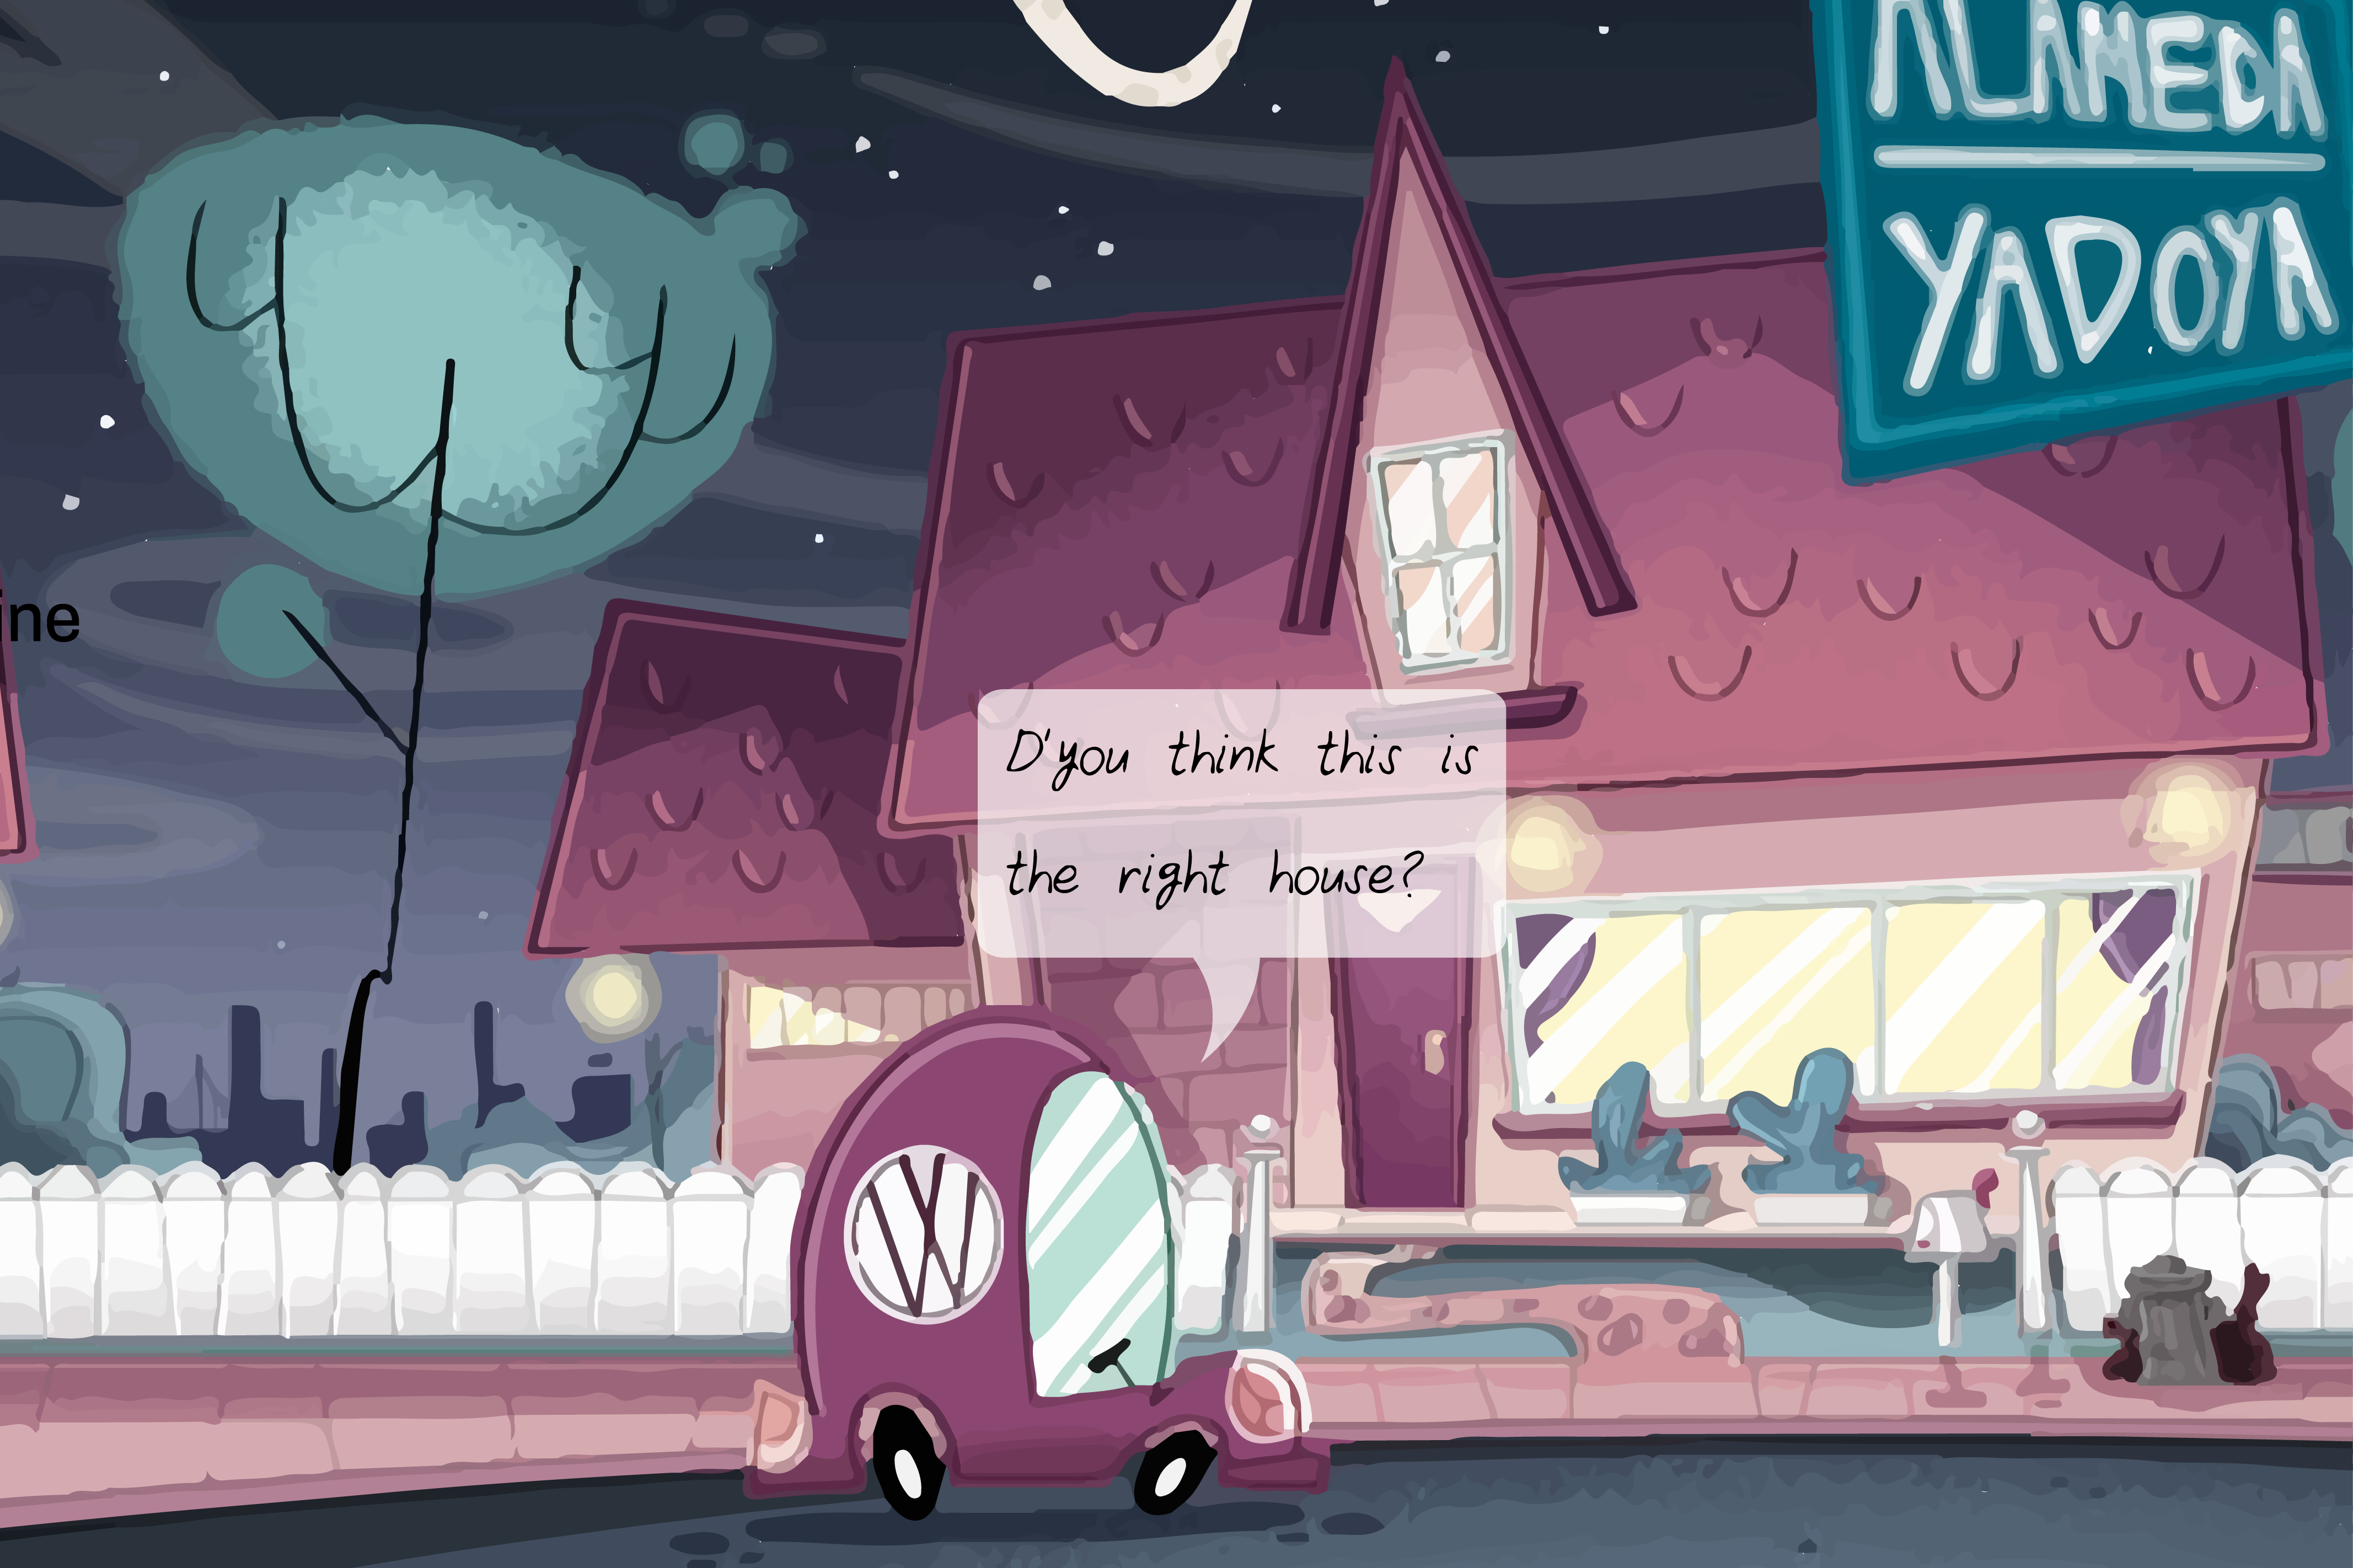
\includegraphics[width=2.3in]{figures/exp1/test-10.png}
% \end{array}$
% \end{center}
% \end{figure}

% \begin{figure}[h]
% \begin{center}$
% \begin{array}{c c}
% 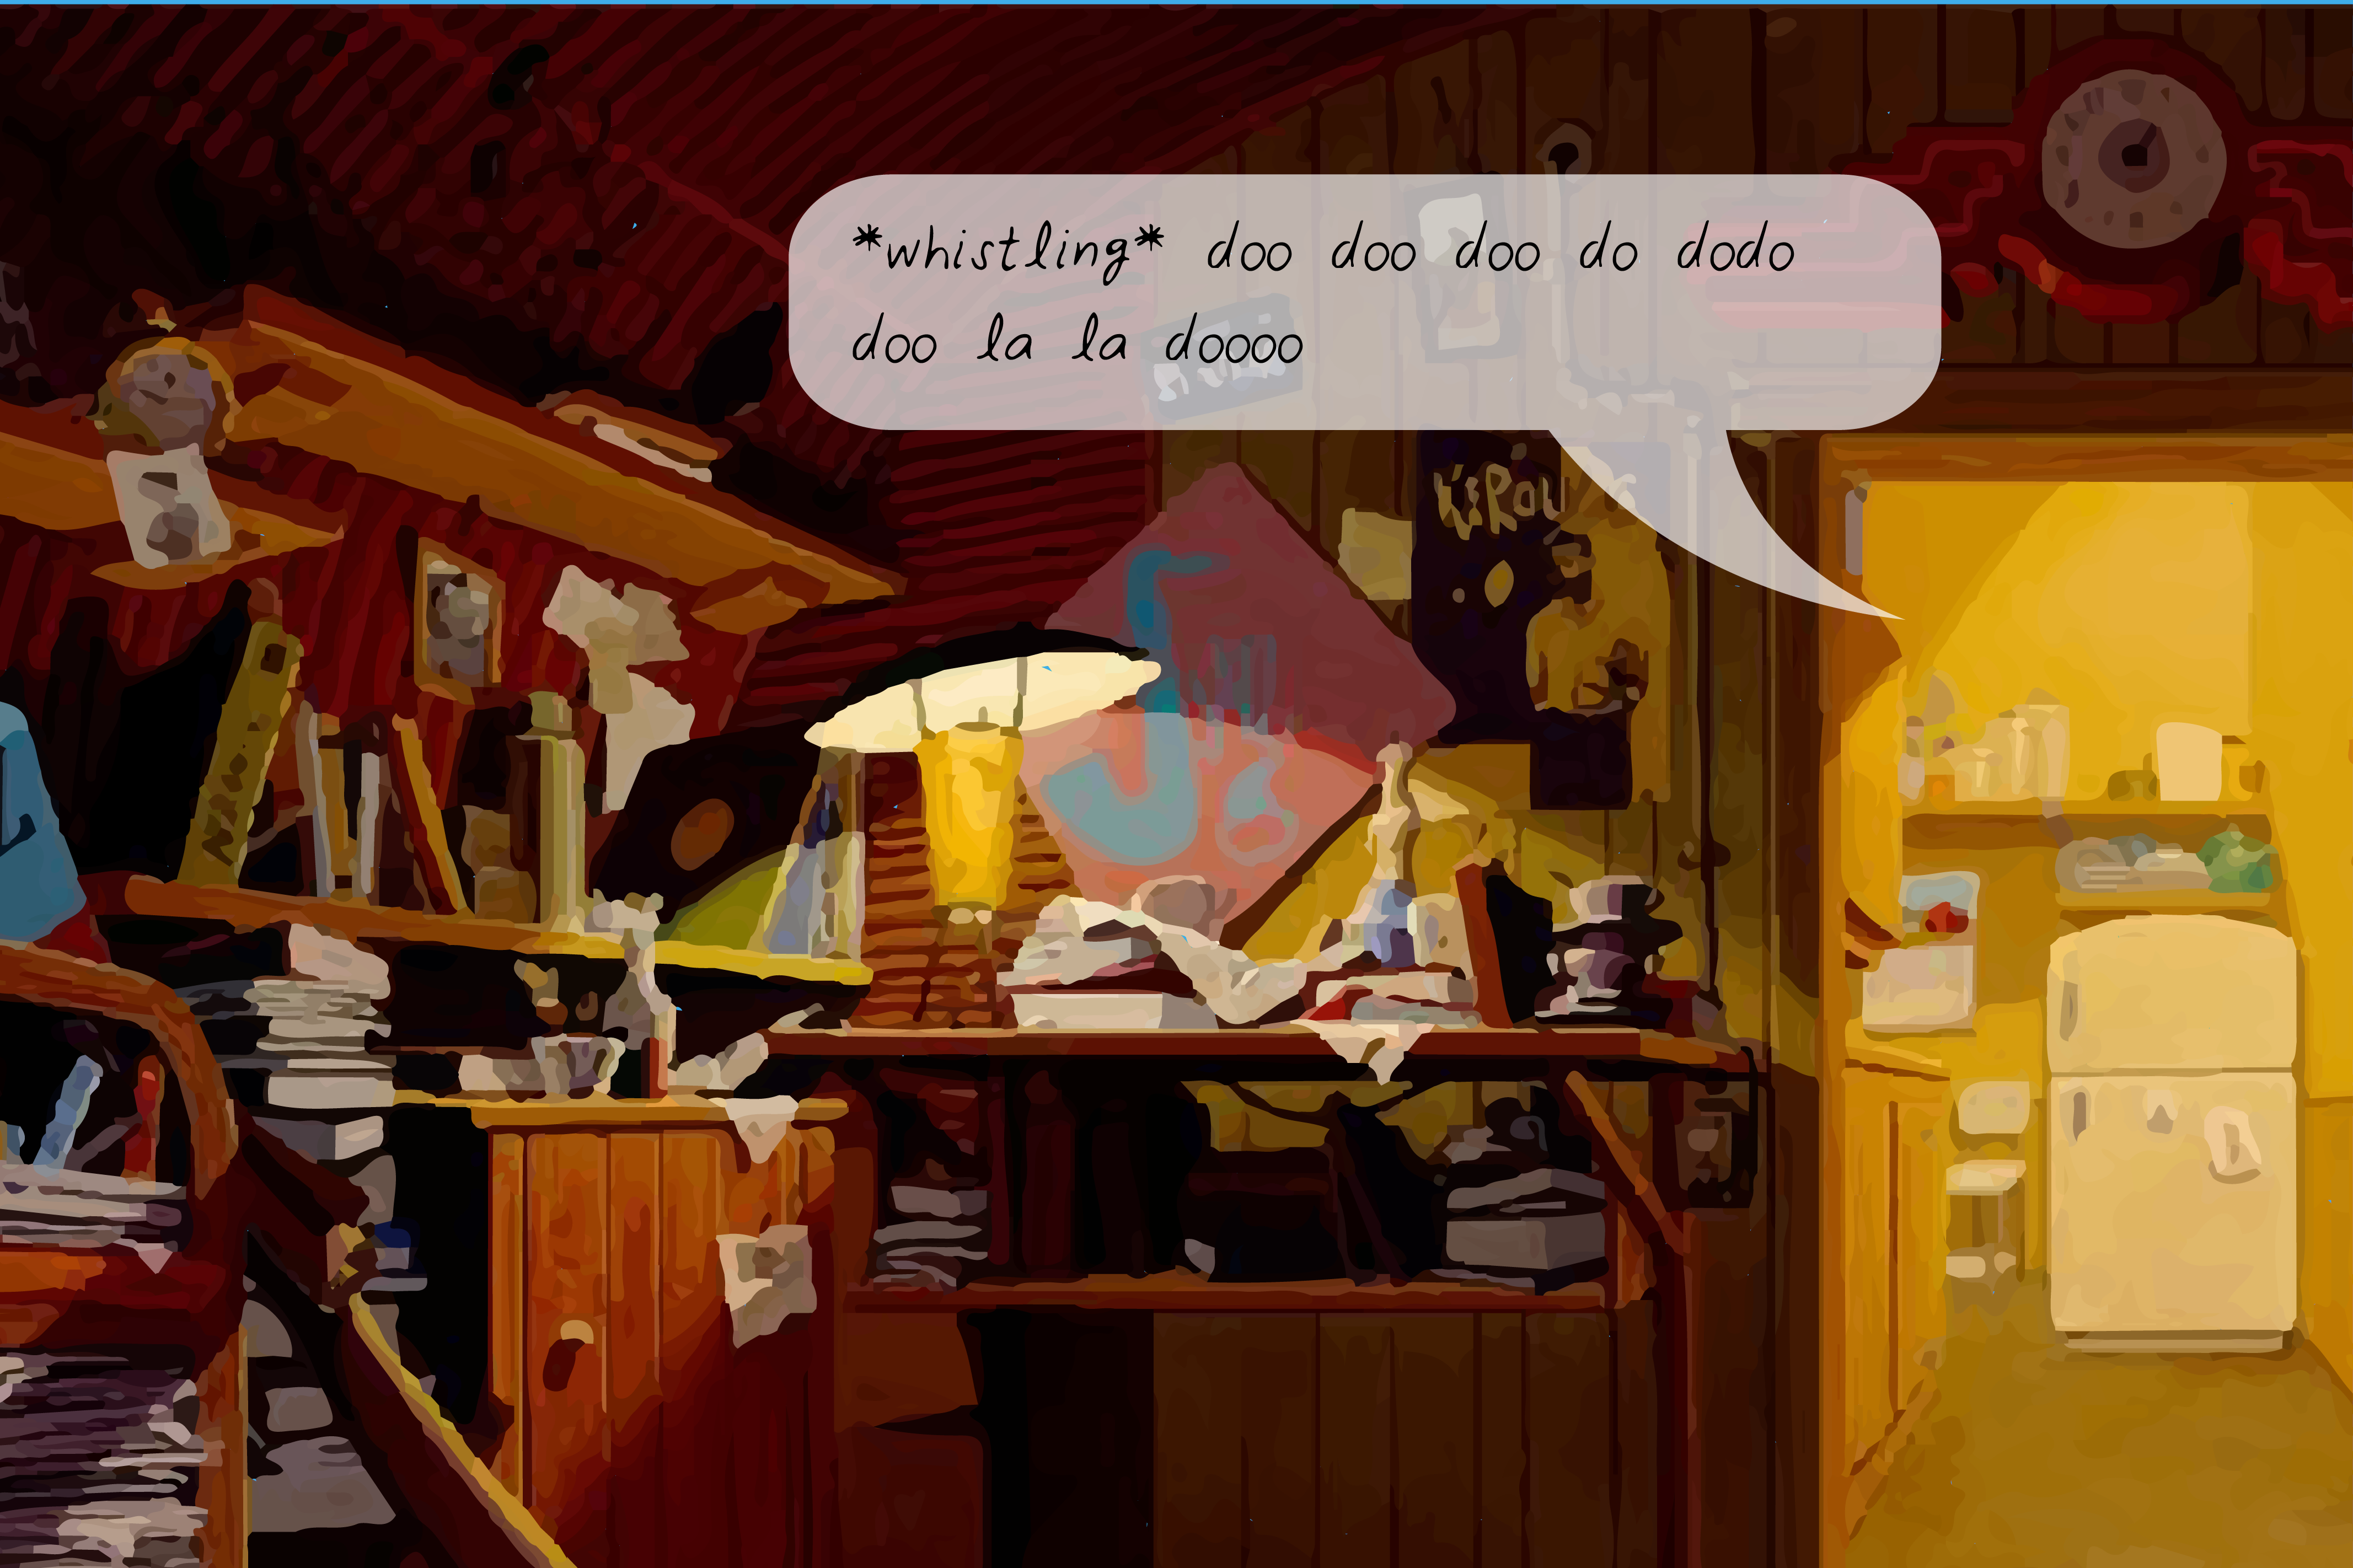
\includegraphics[width=2.5in]{figures/exp1/test-11.png} &
% 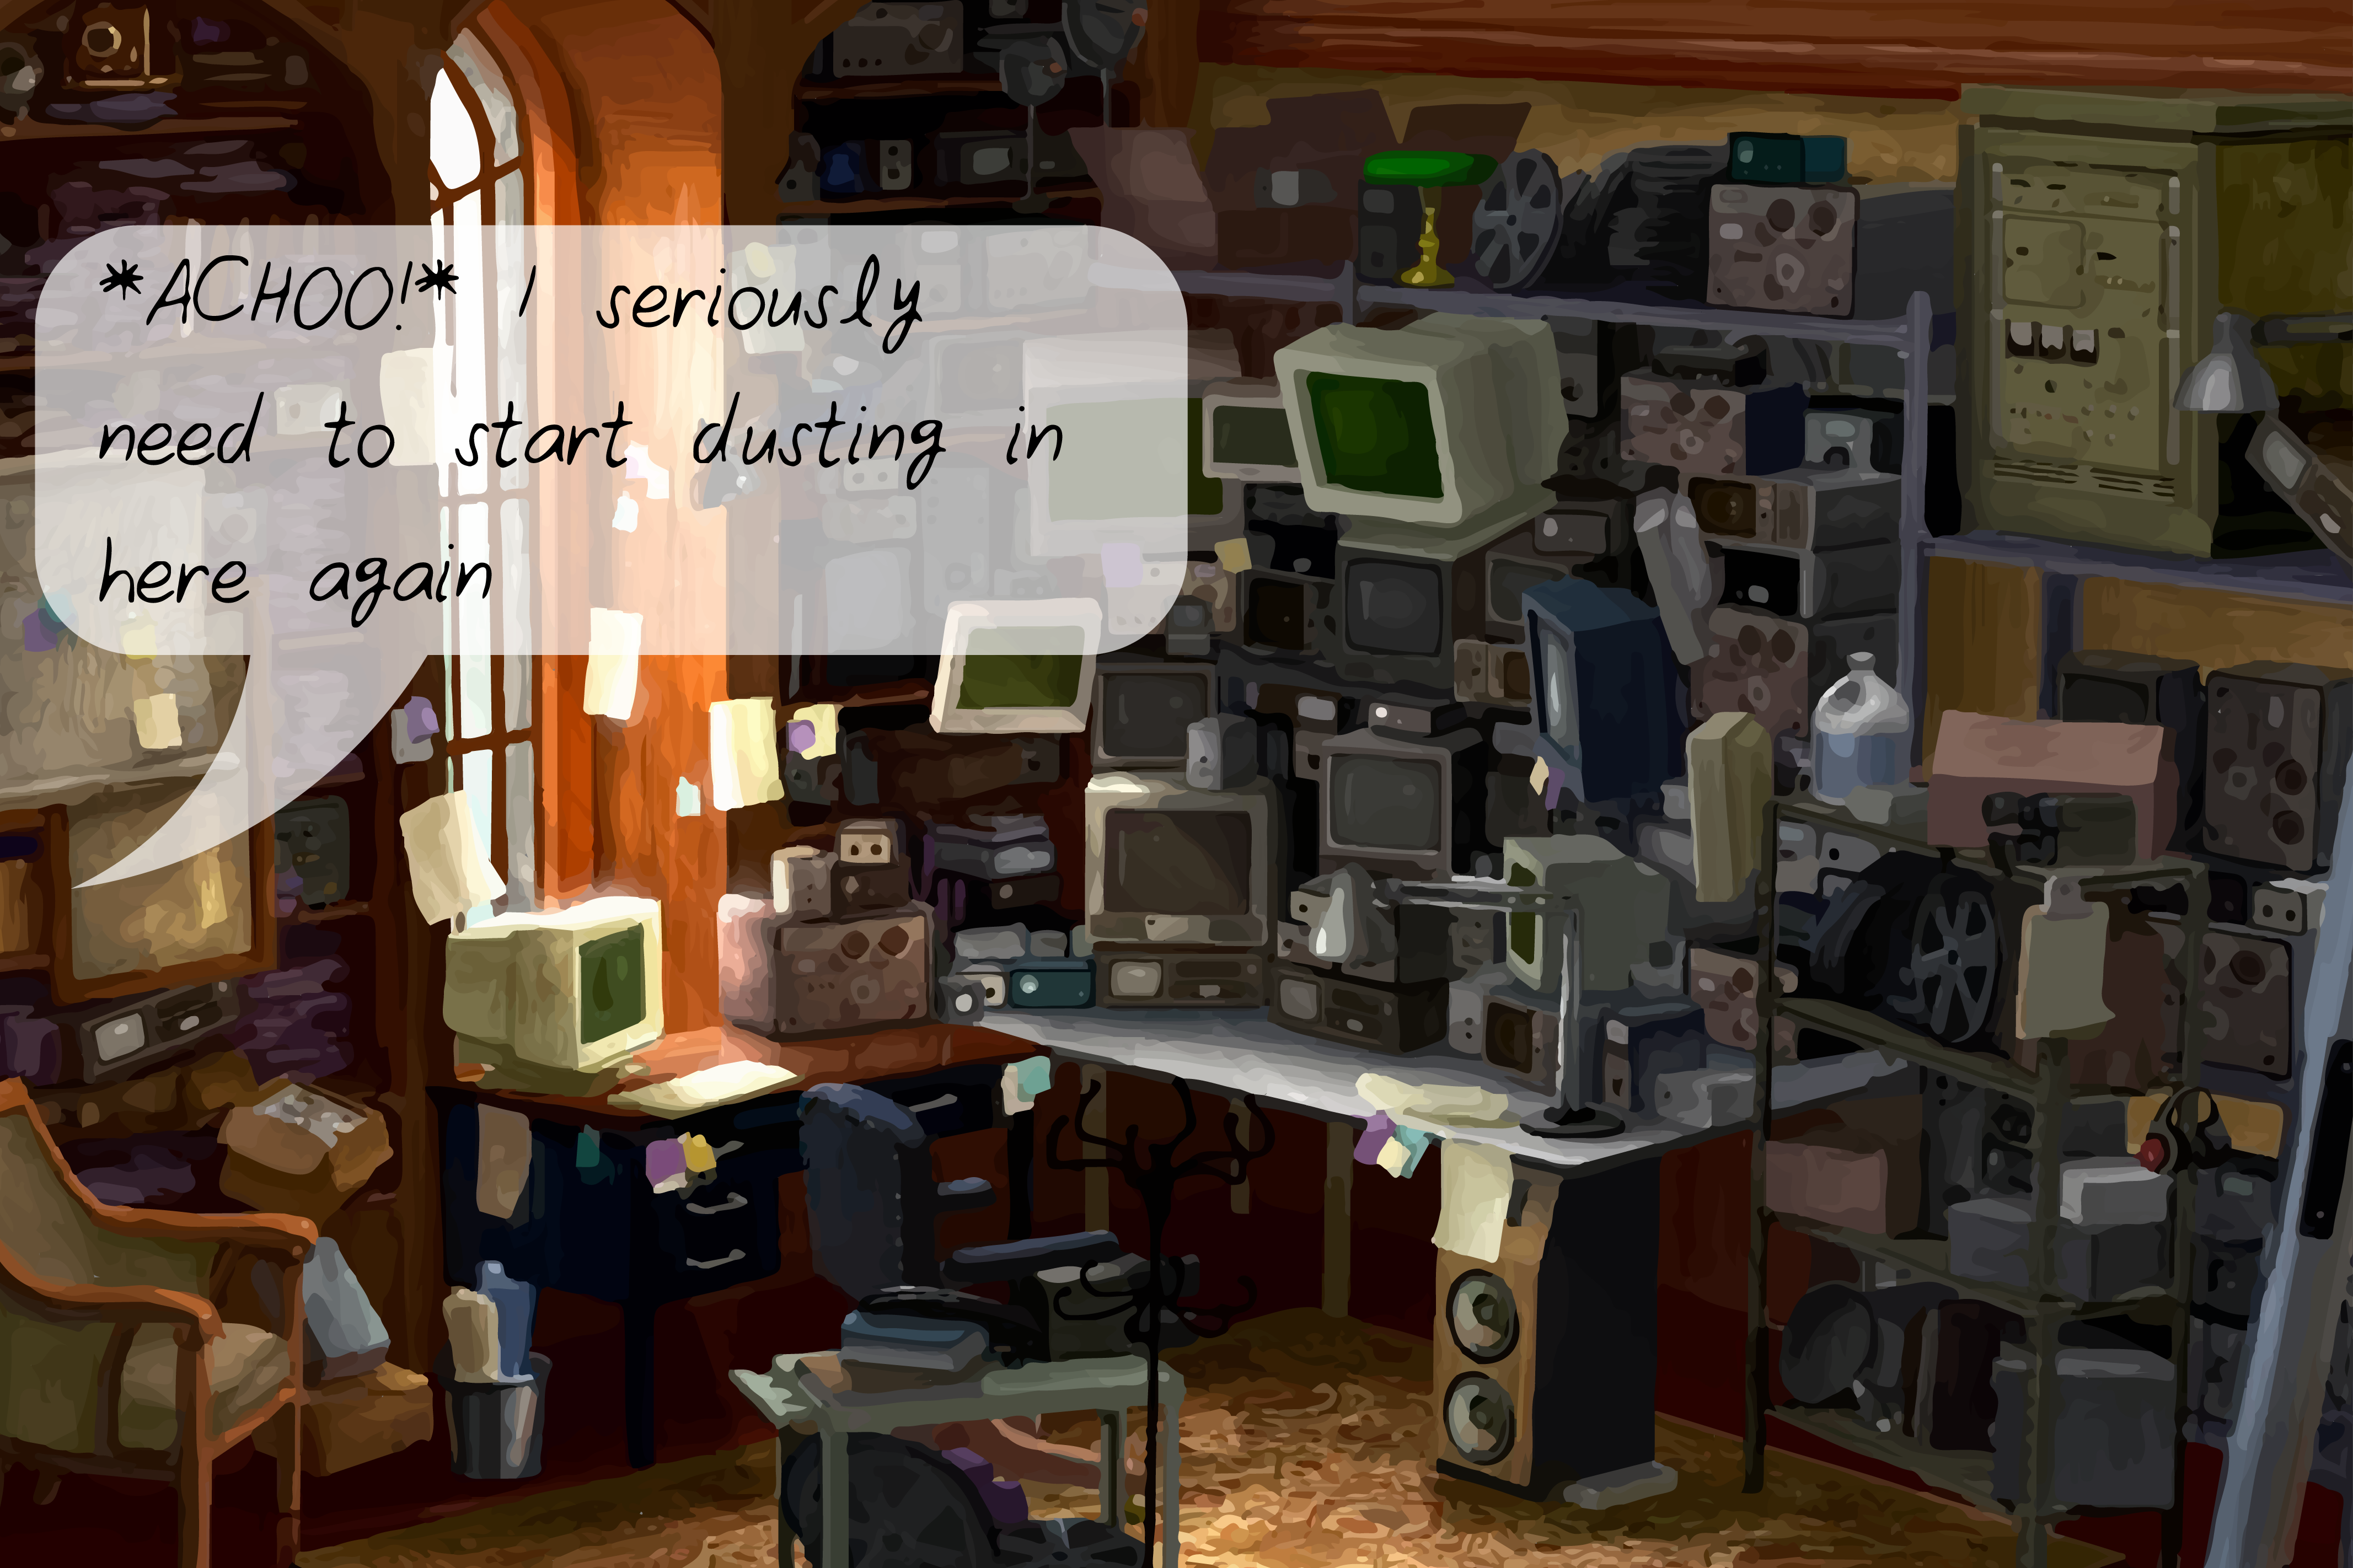
\includegraphics[width=2.5in]{figures/exp1/test-12.png} \\ 
% 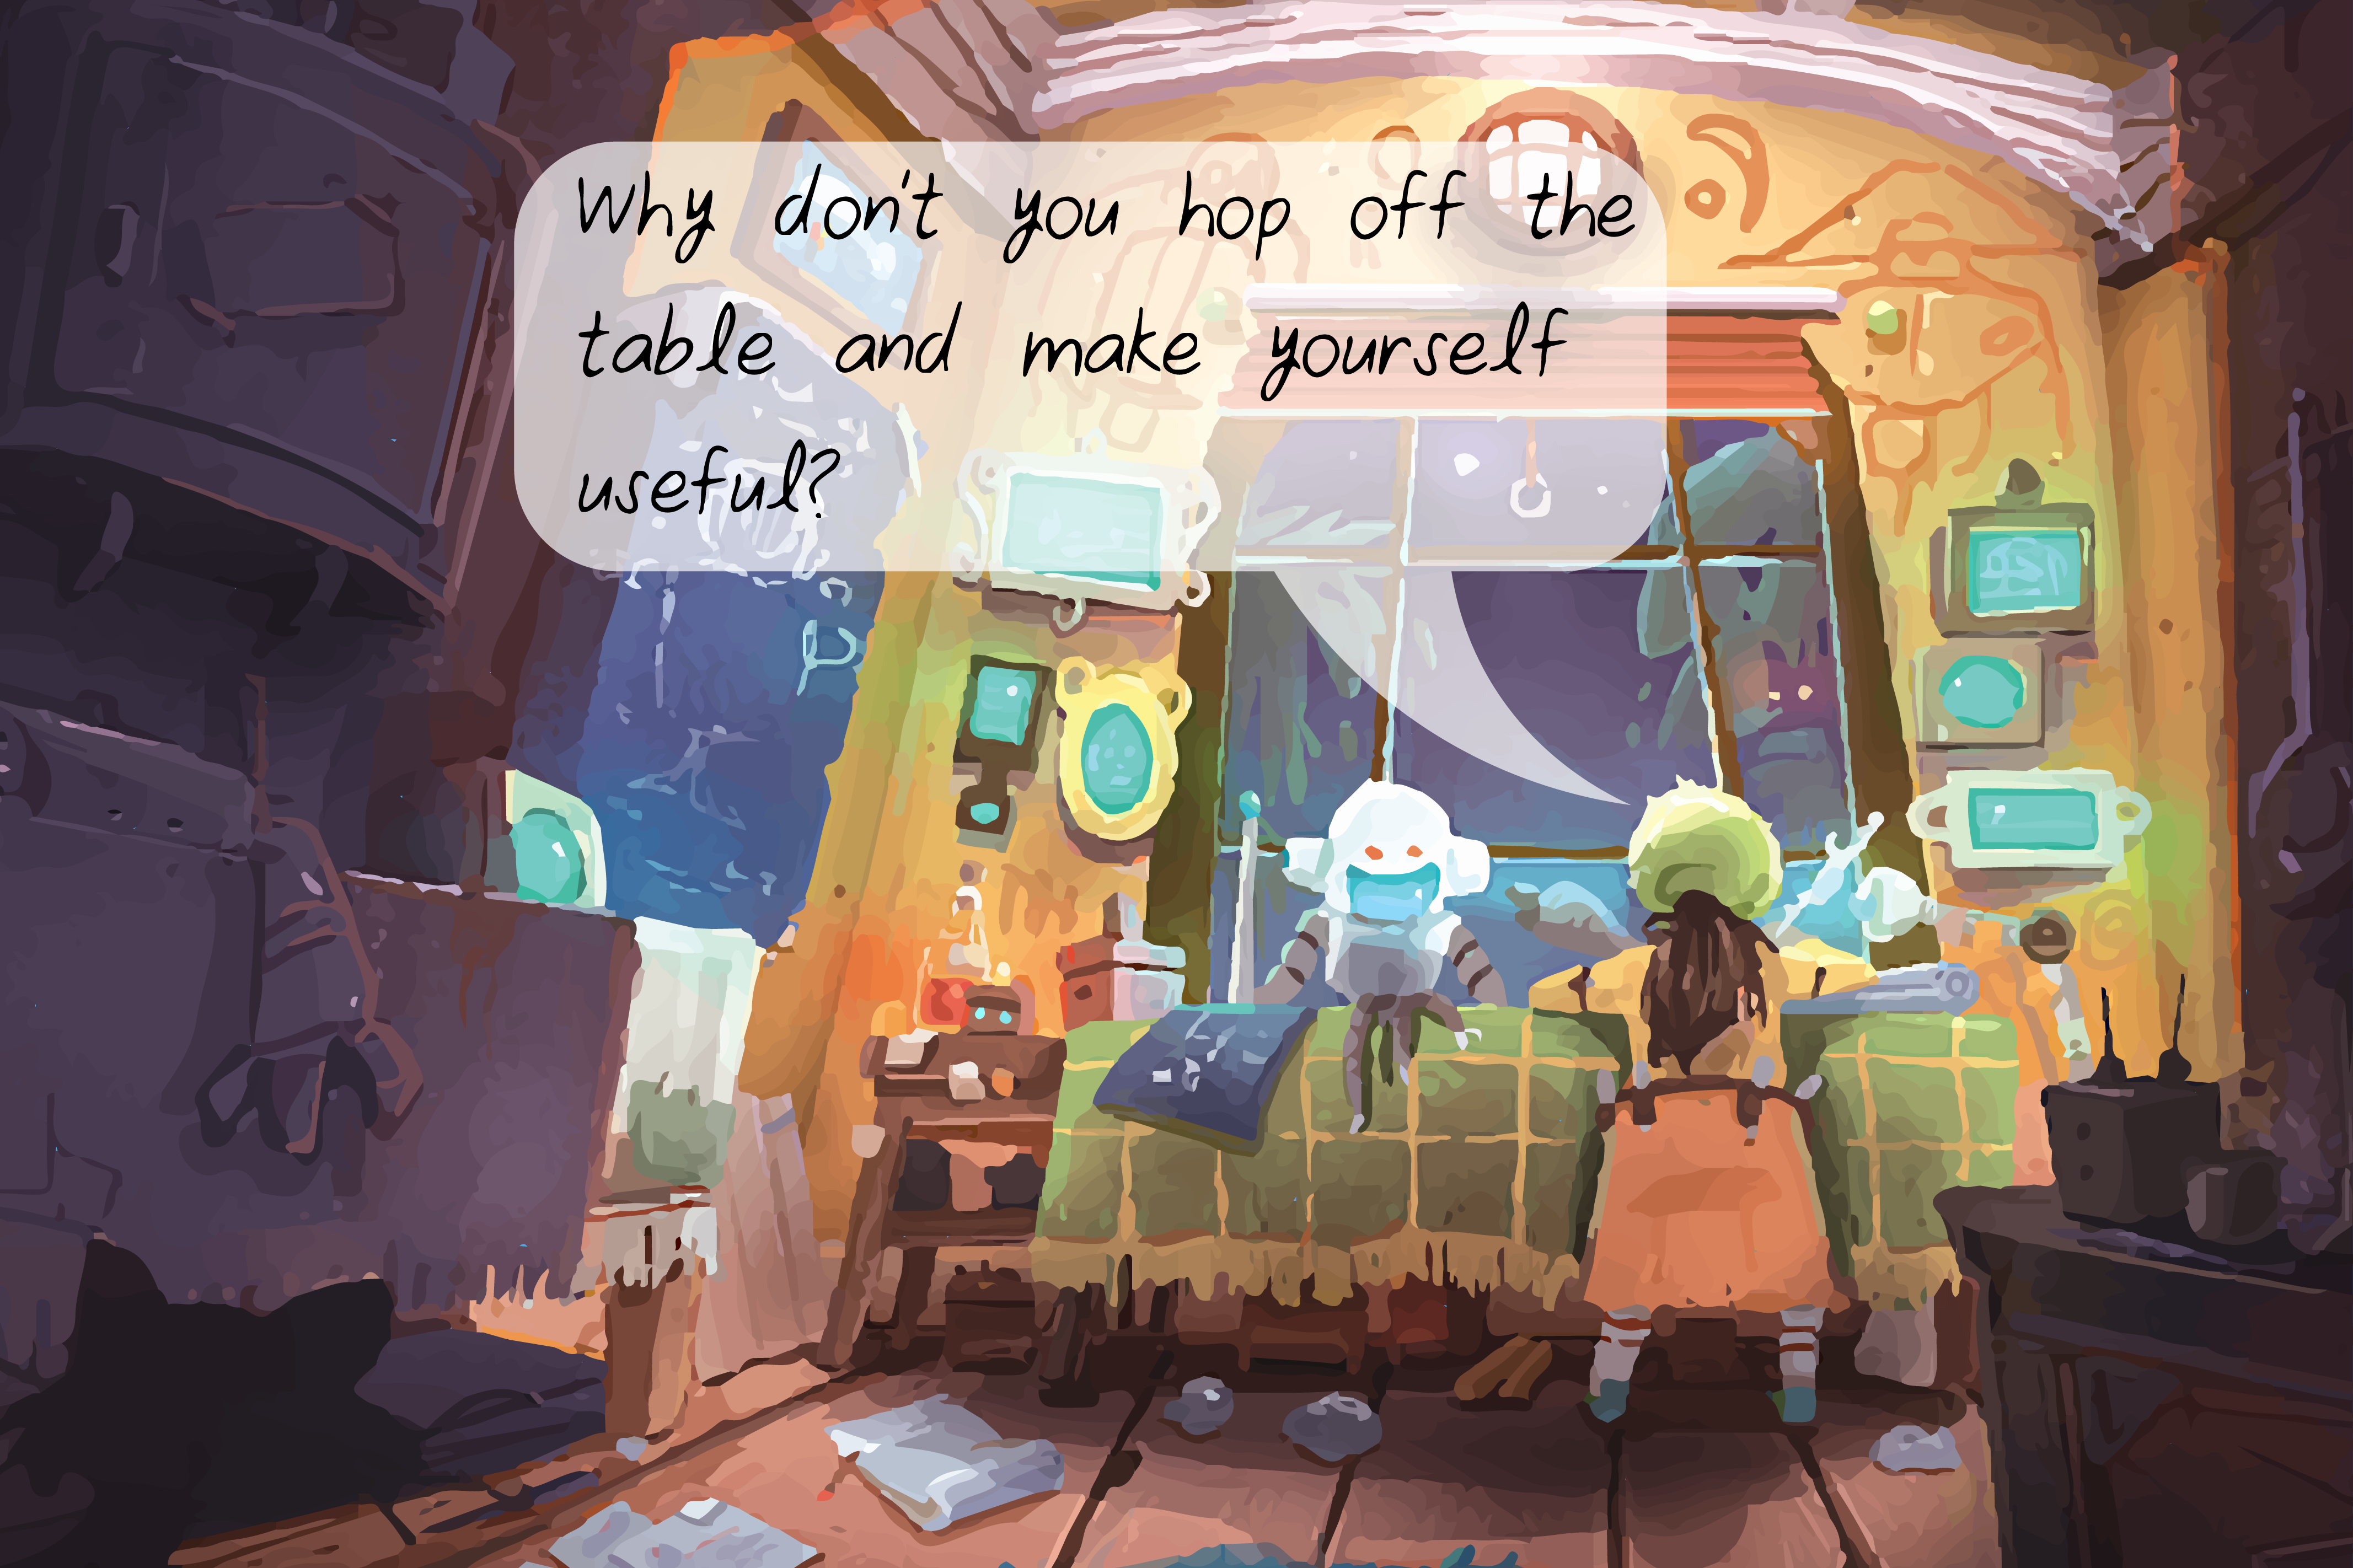
\includegraphics[width=2.5in]{figures/exp1/test-13.png} &
% 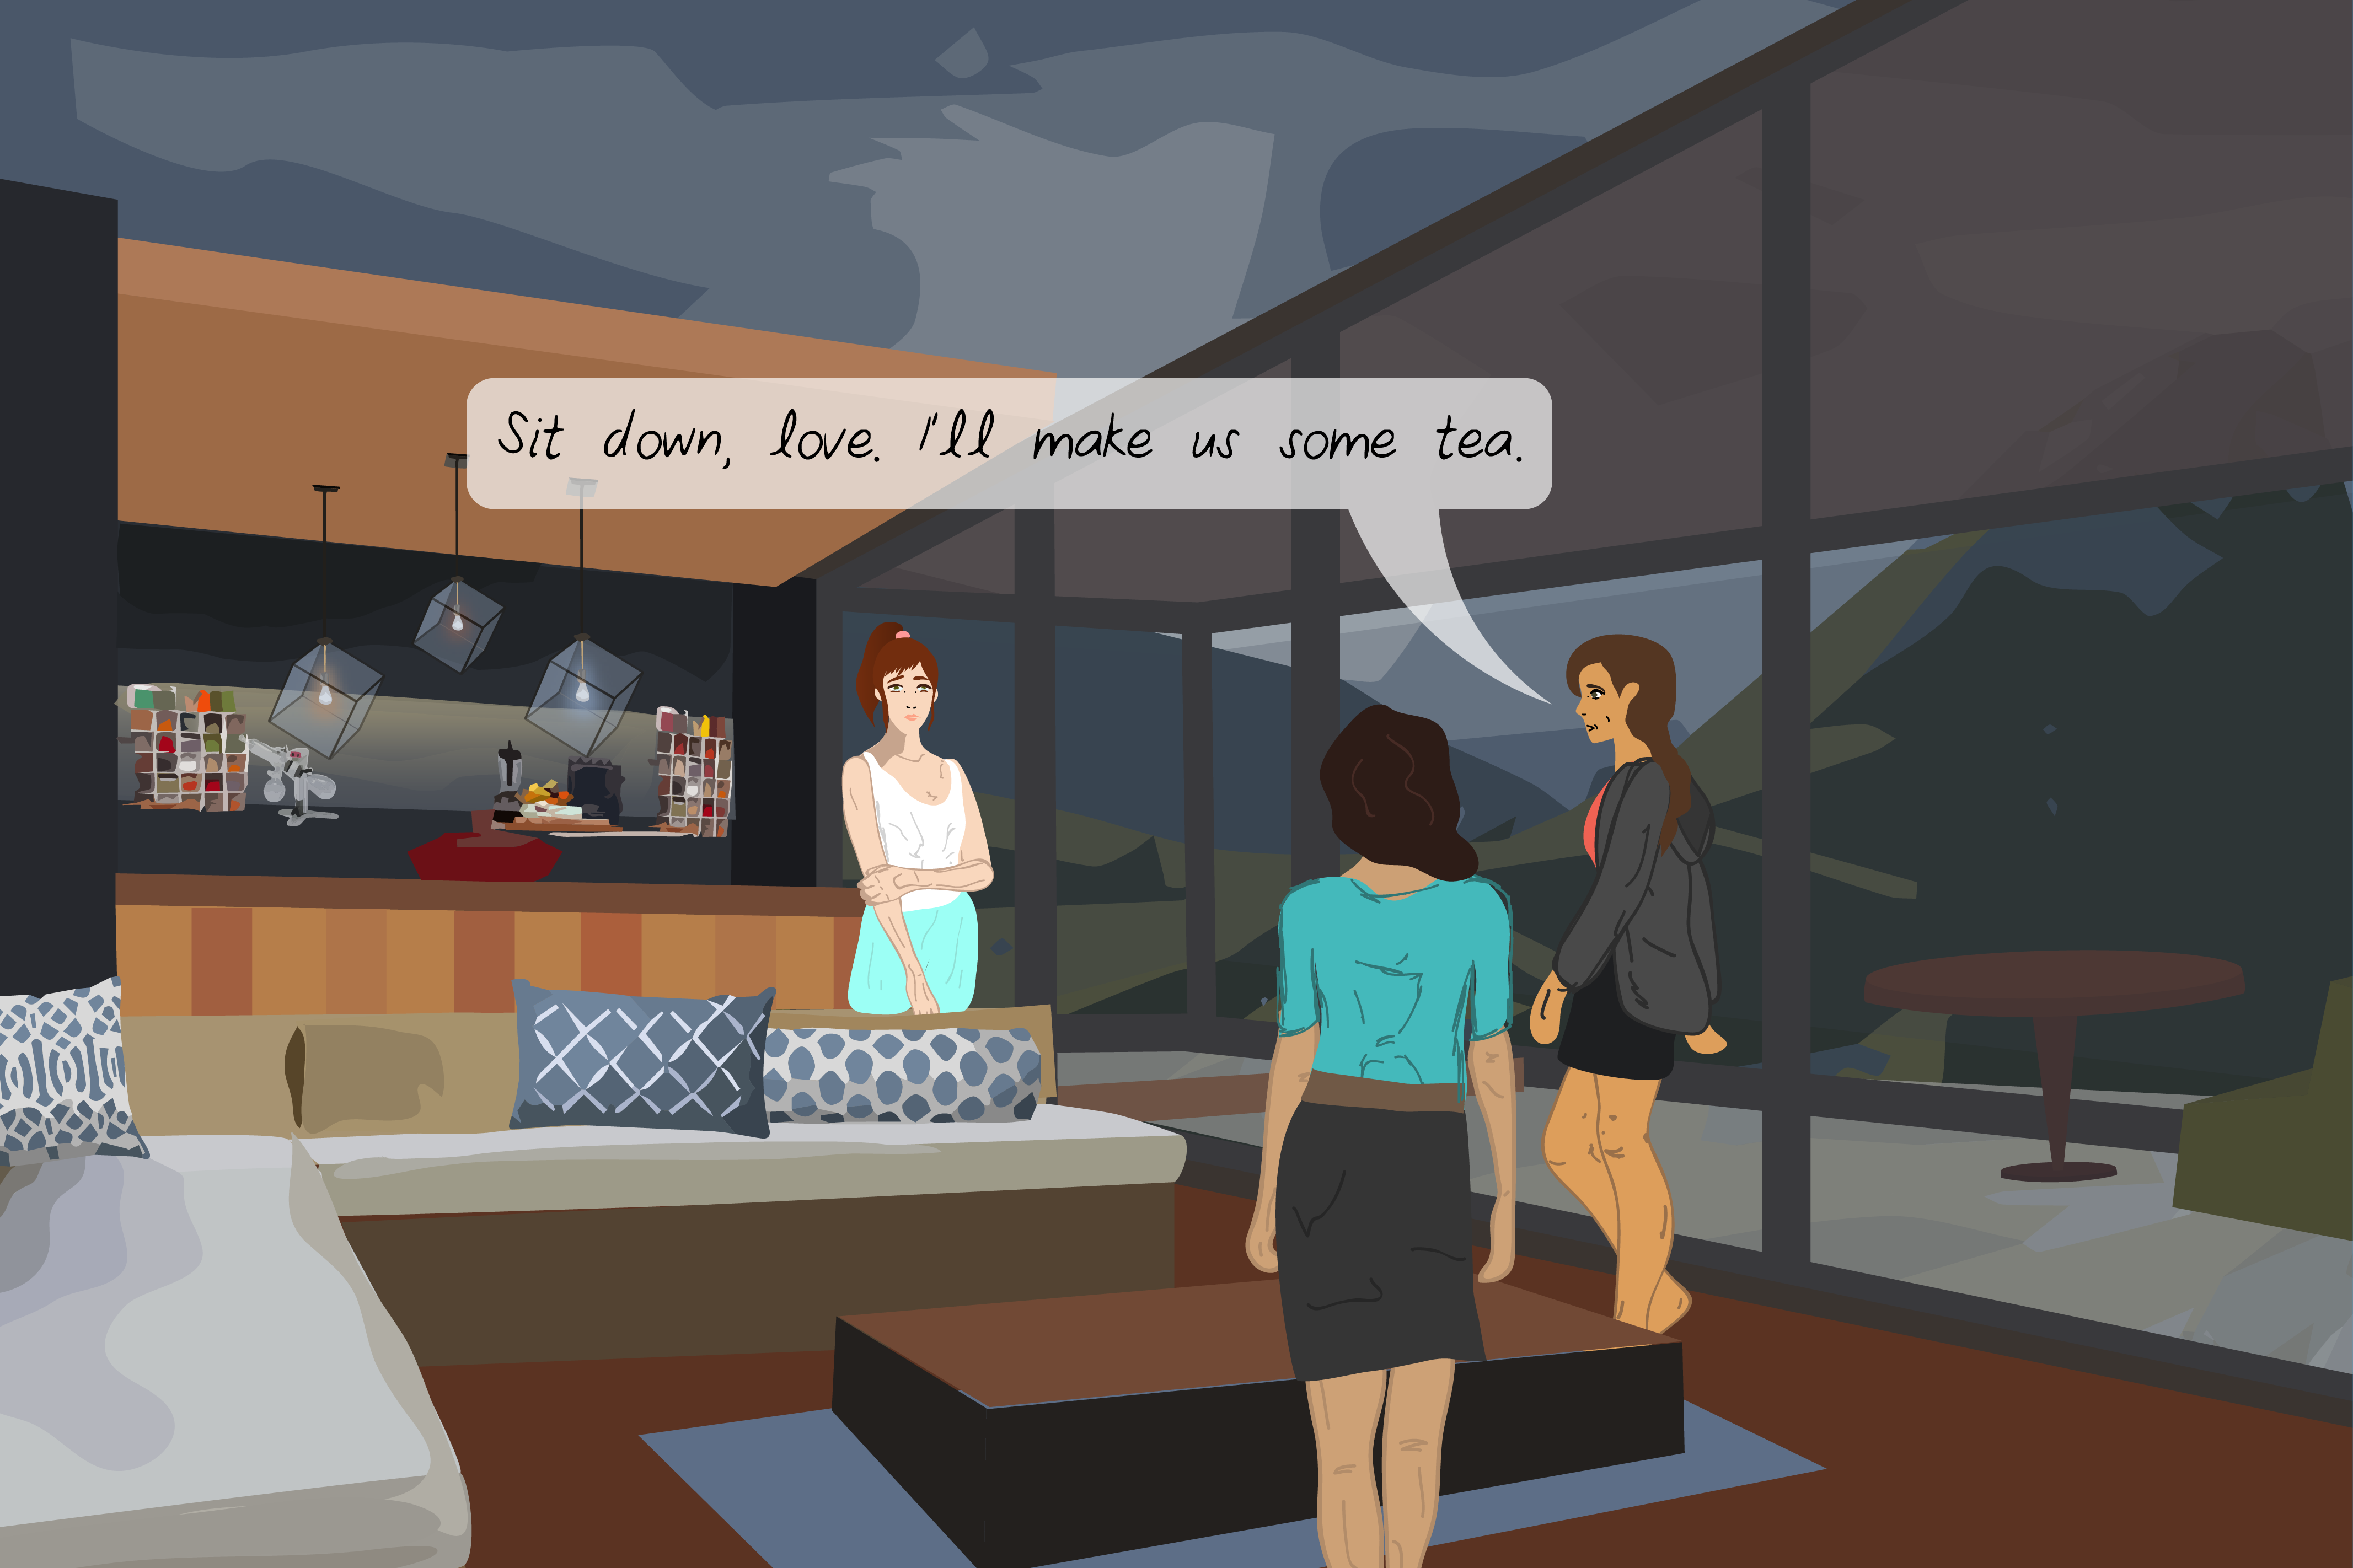
\includegraphics[width=2.5in]{figures/exp1/test-14.png} \\ 
% 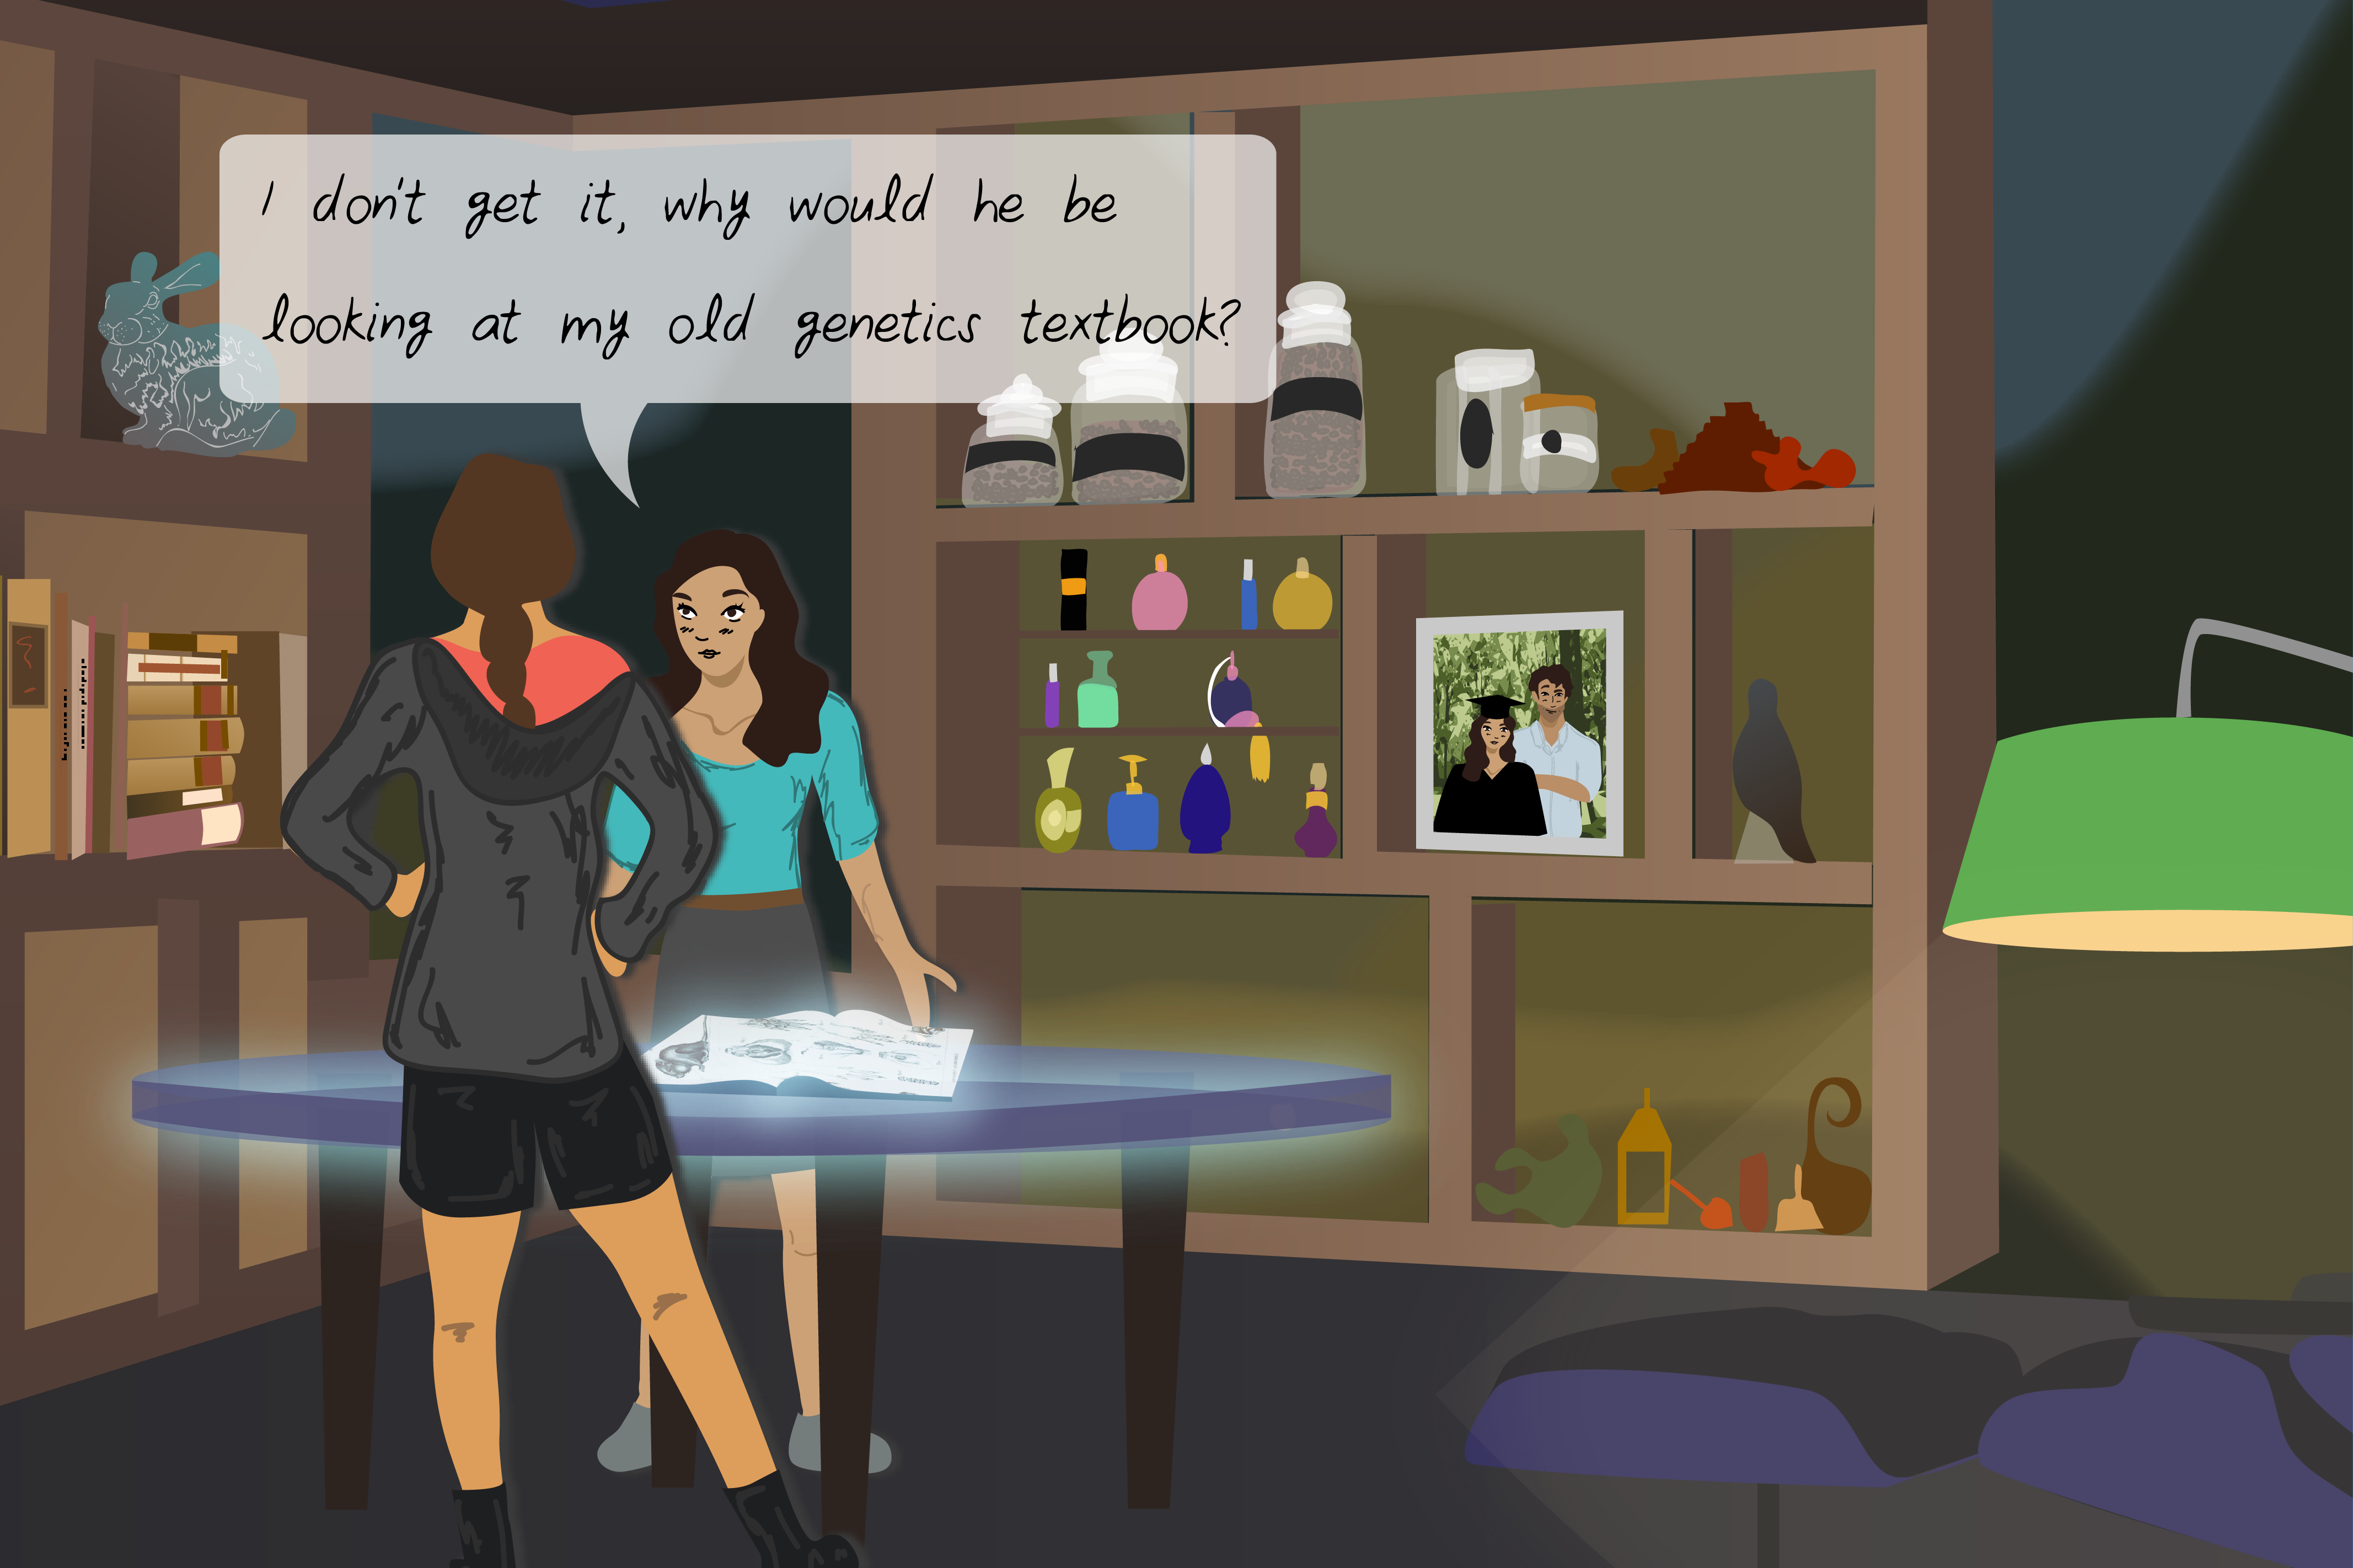
\includegraphics[width=2.5in]{figures/exp1/test-15.png} &
% 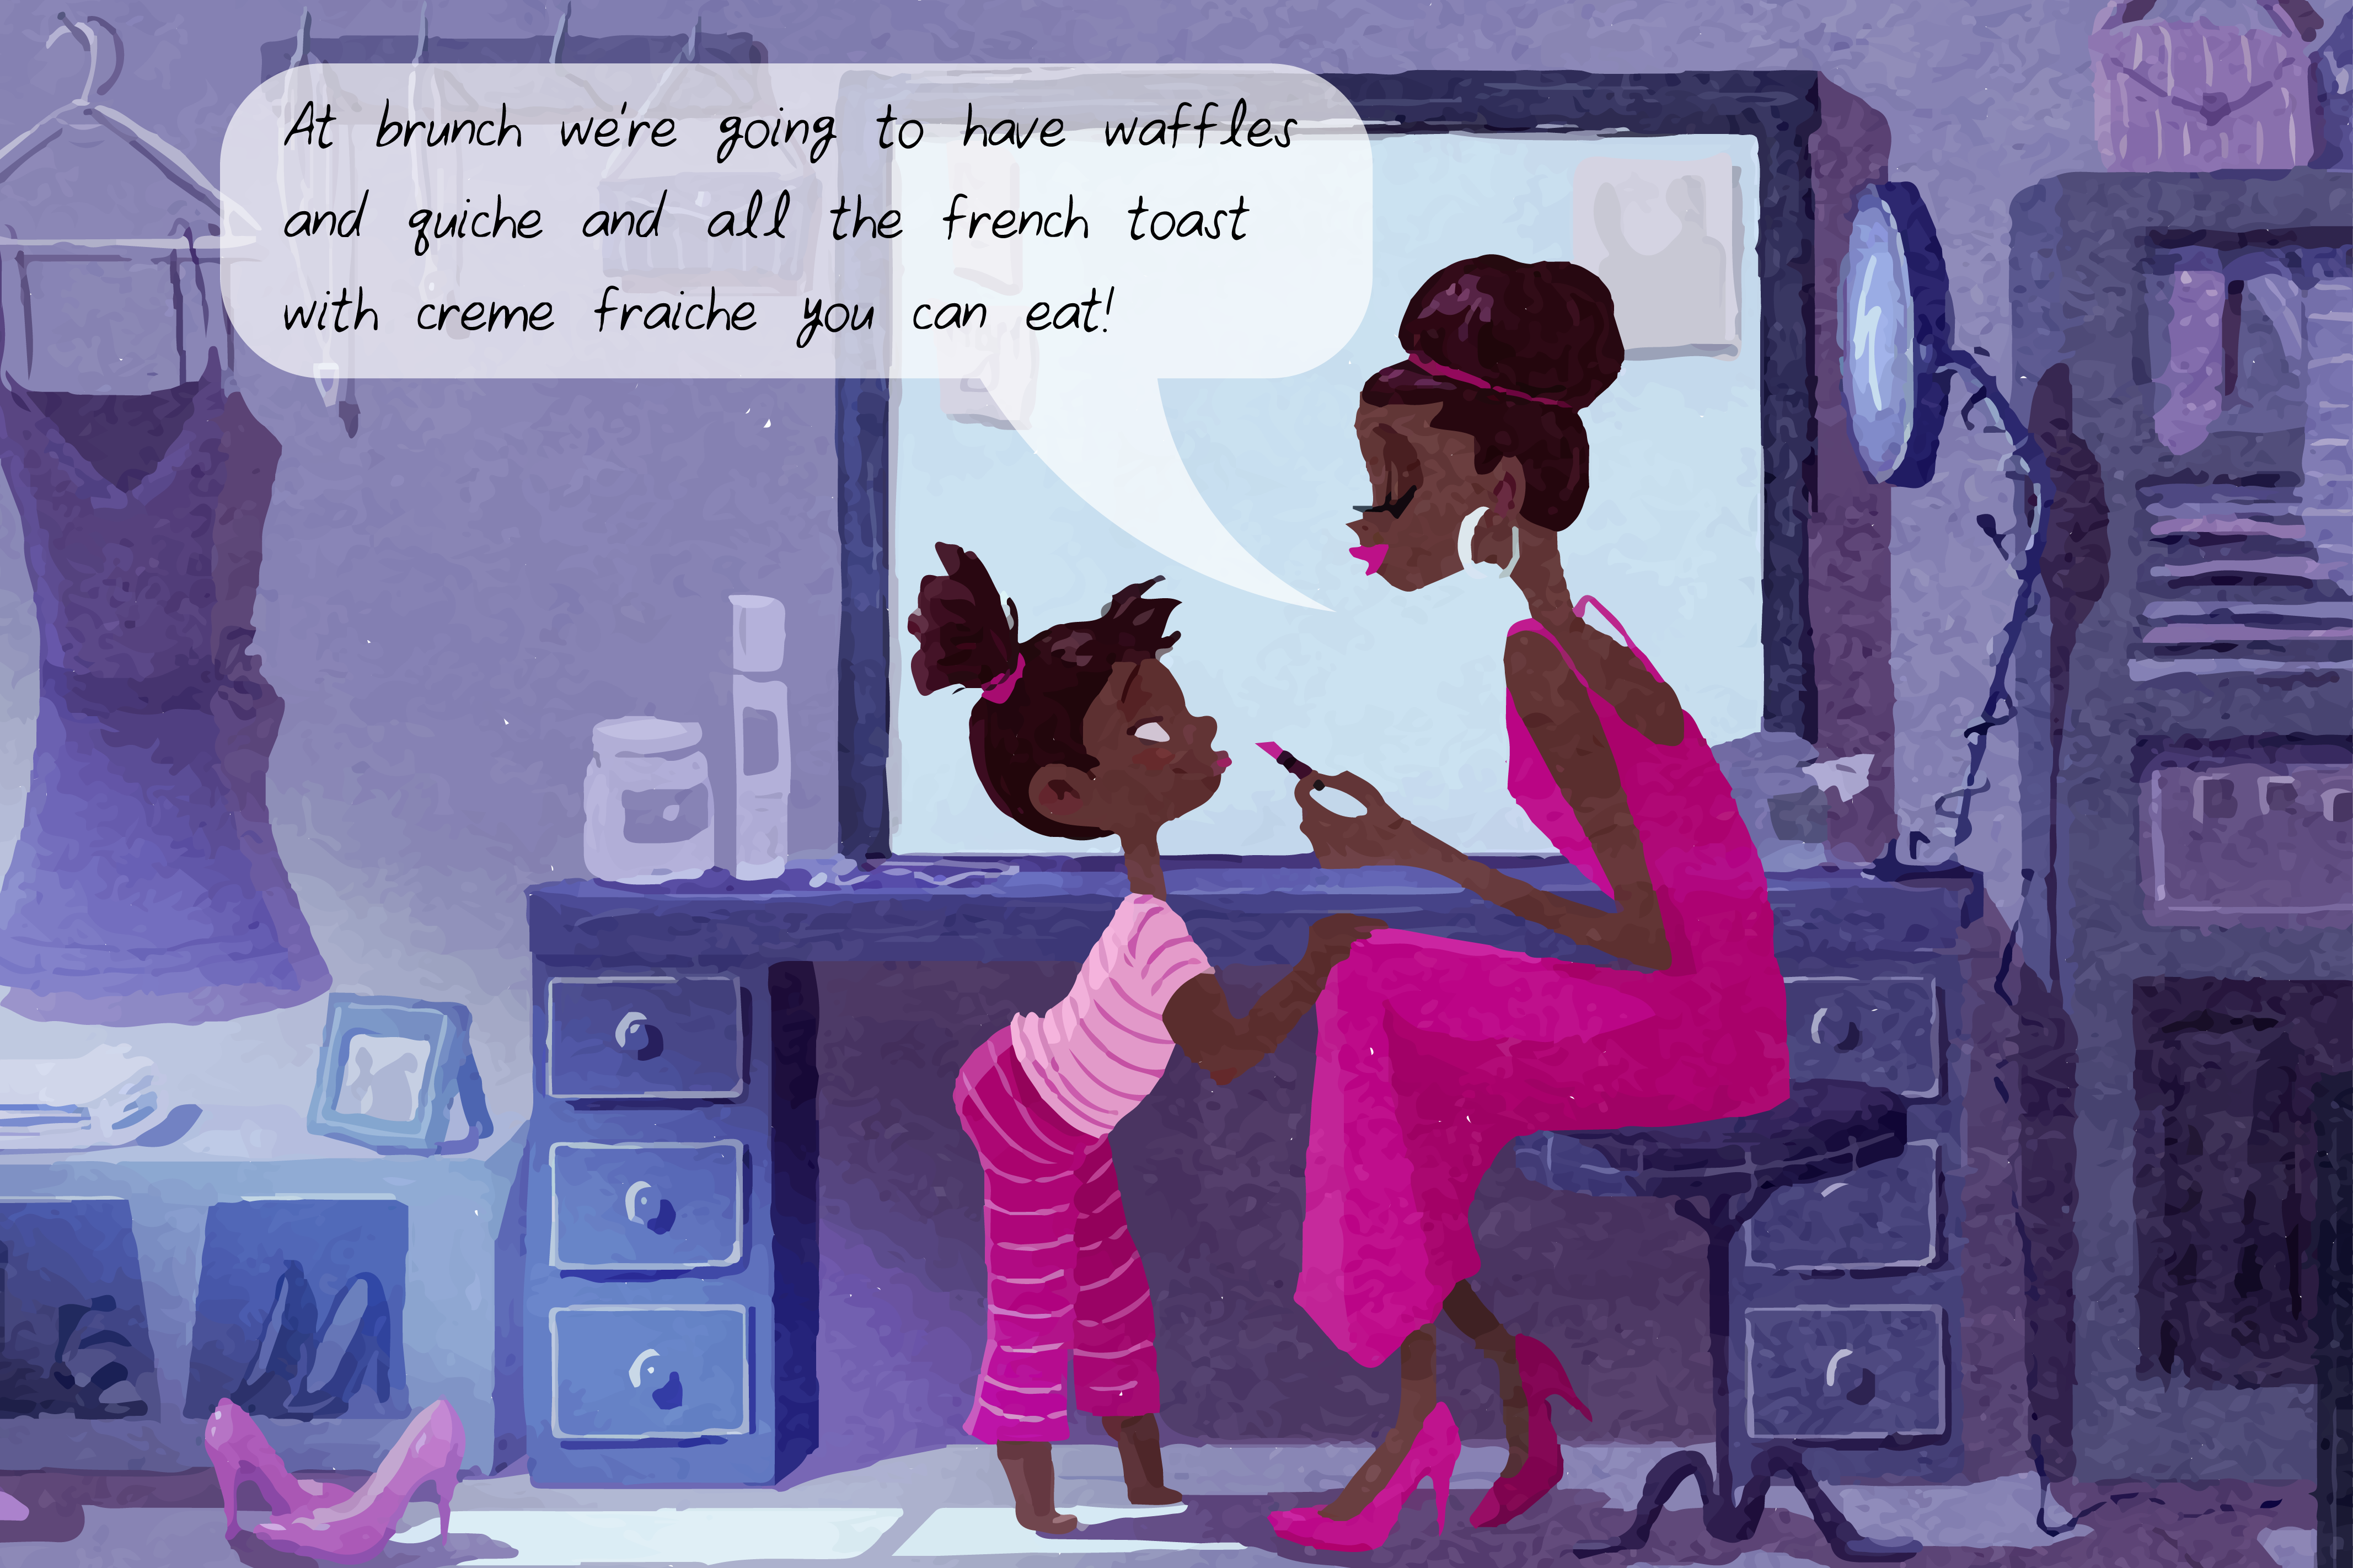
\includegraphics[width=2.5in]{figures/exp1/test-16.png} \\ 
% 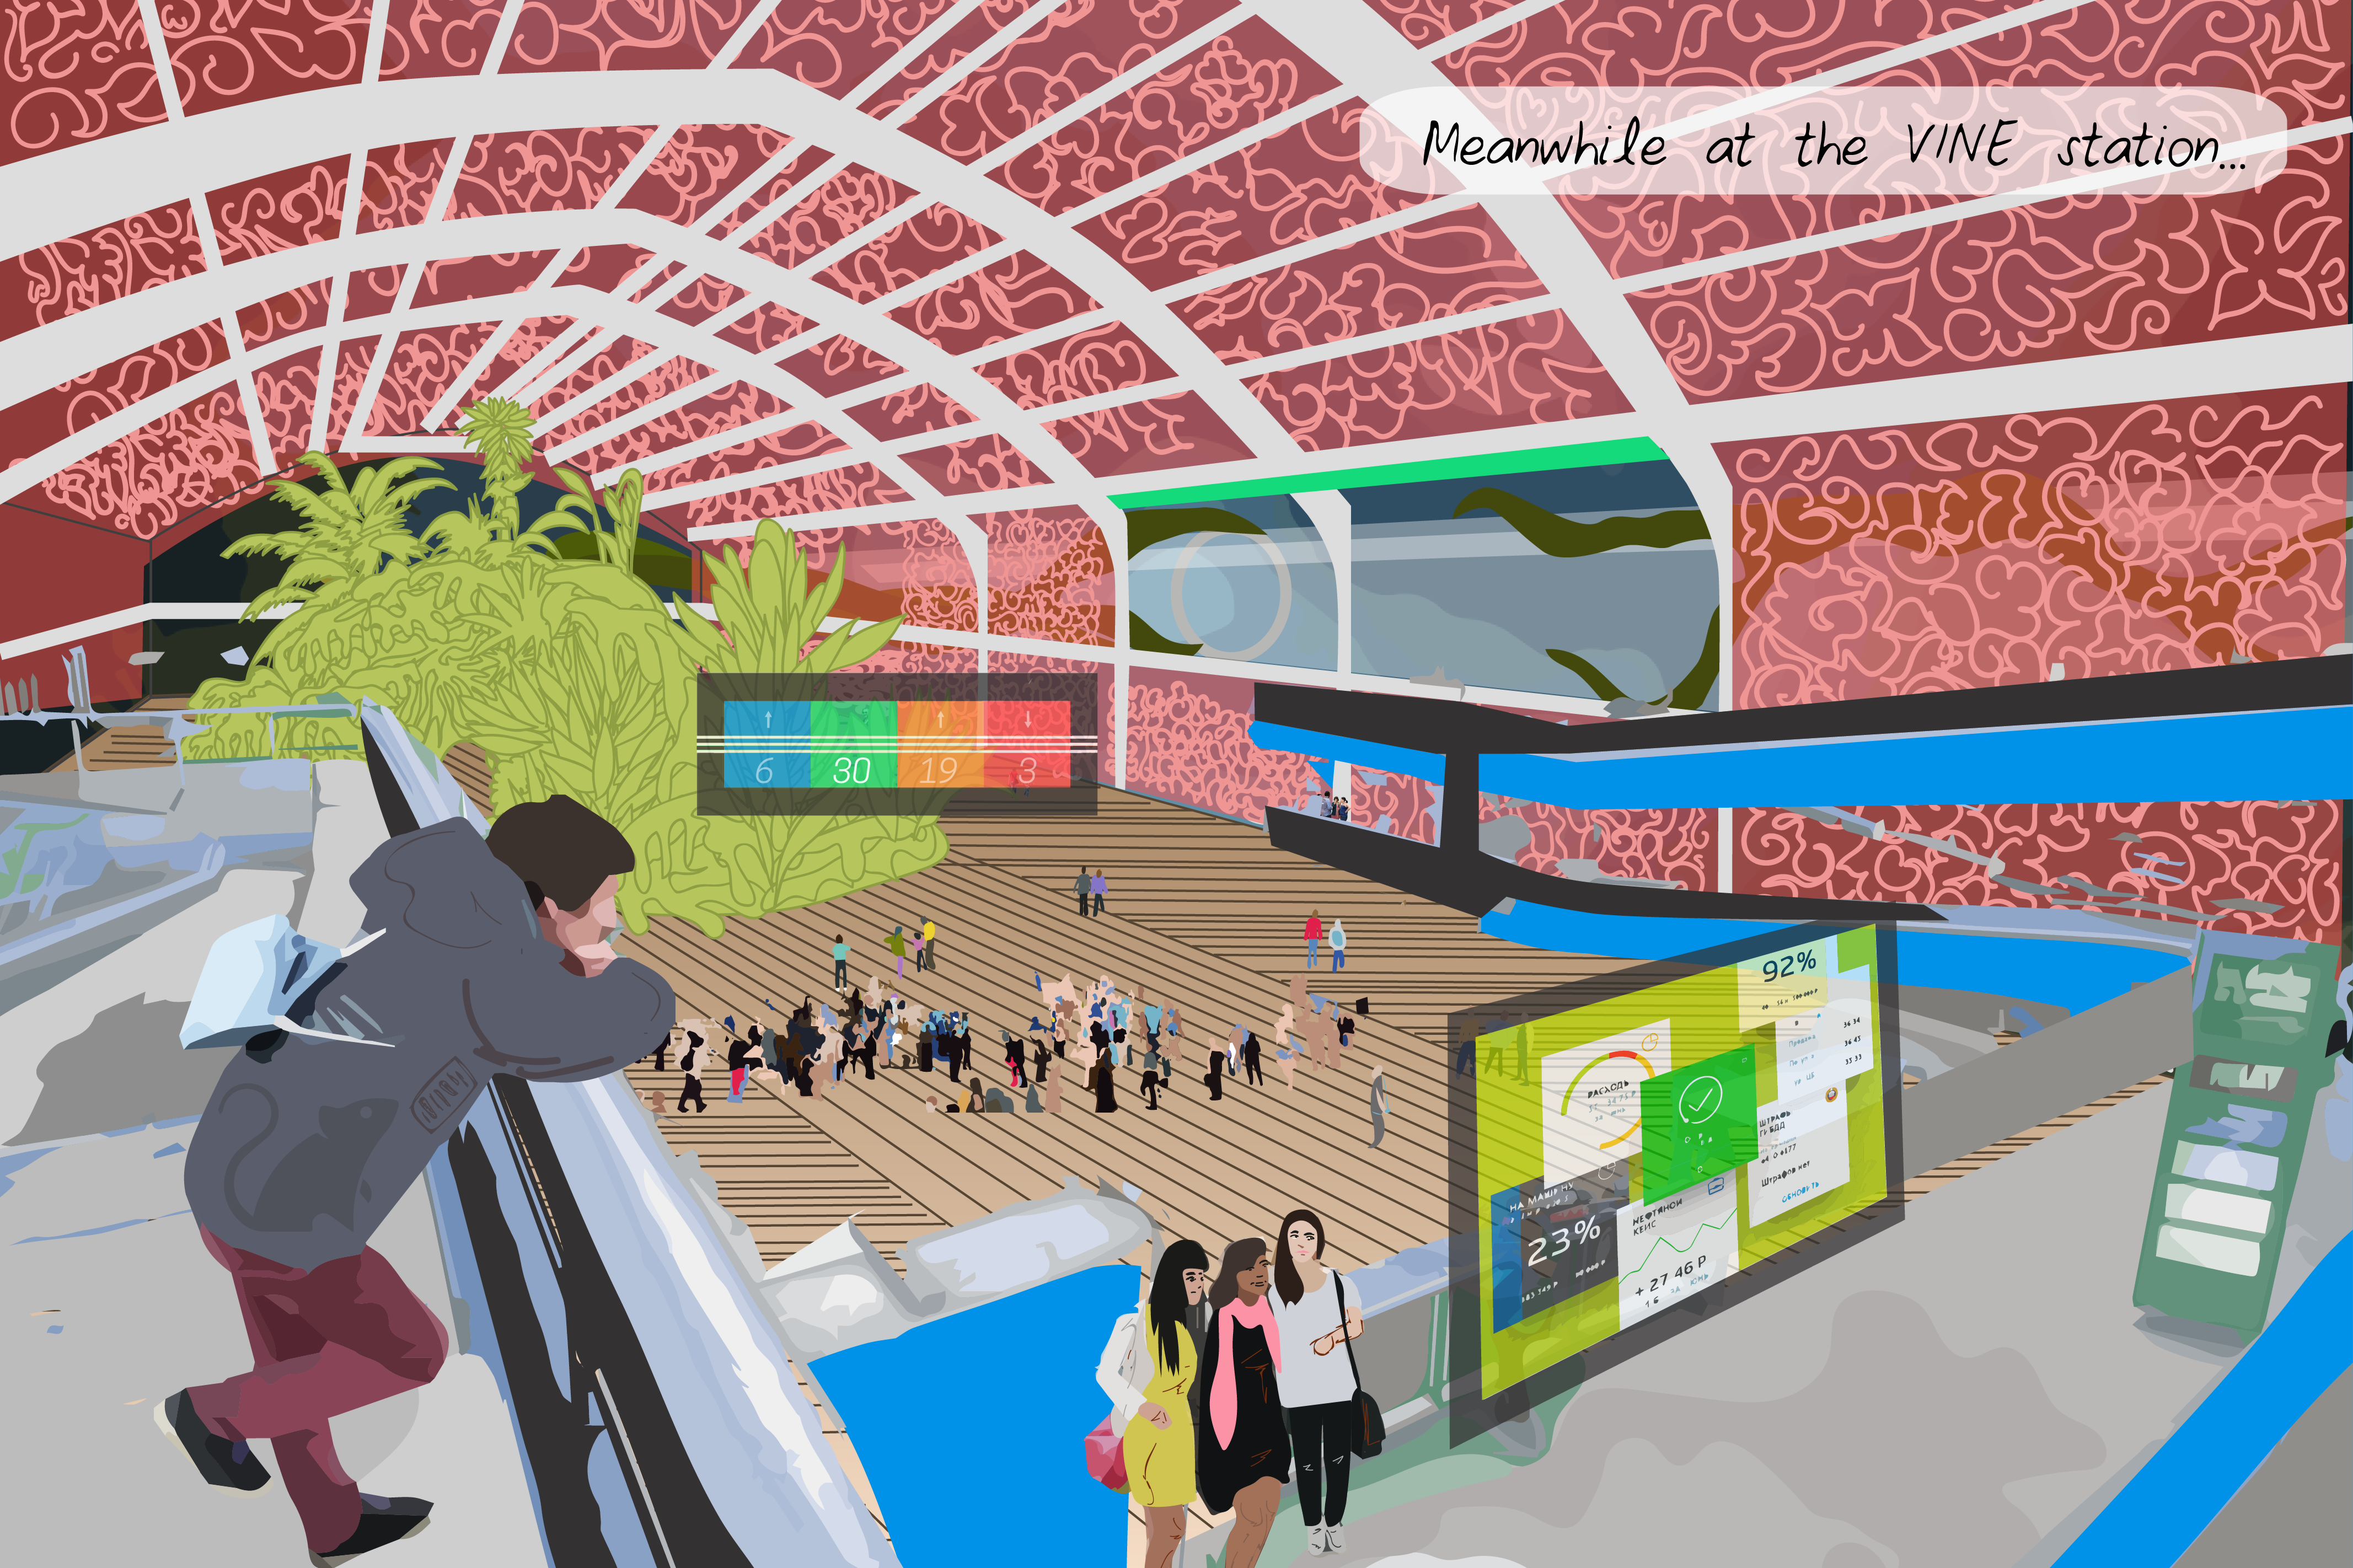
\includegraphics[width=2.5in]{figures/exp1/test-17.png} &
% \includegraphics[width=2.5in]{figures/exp1/test-18.png} \\ 
% 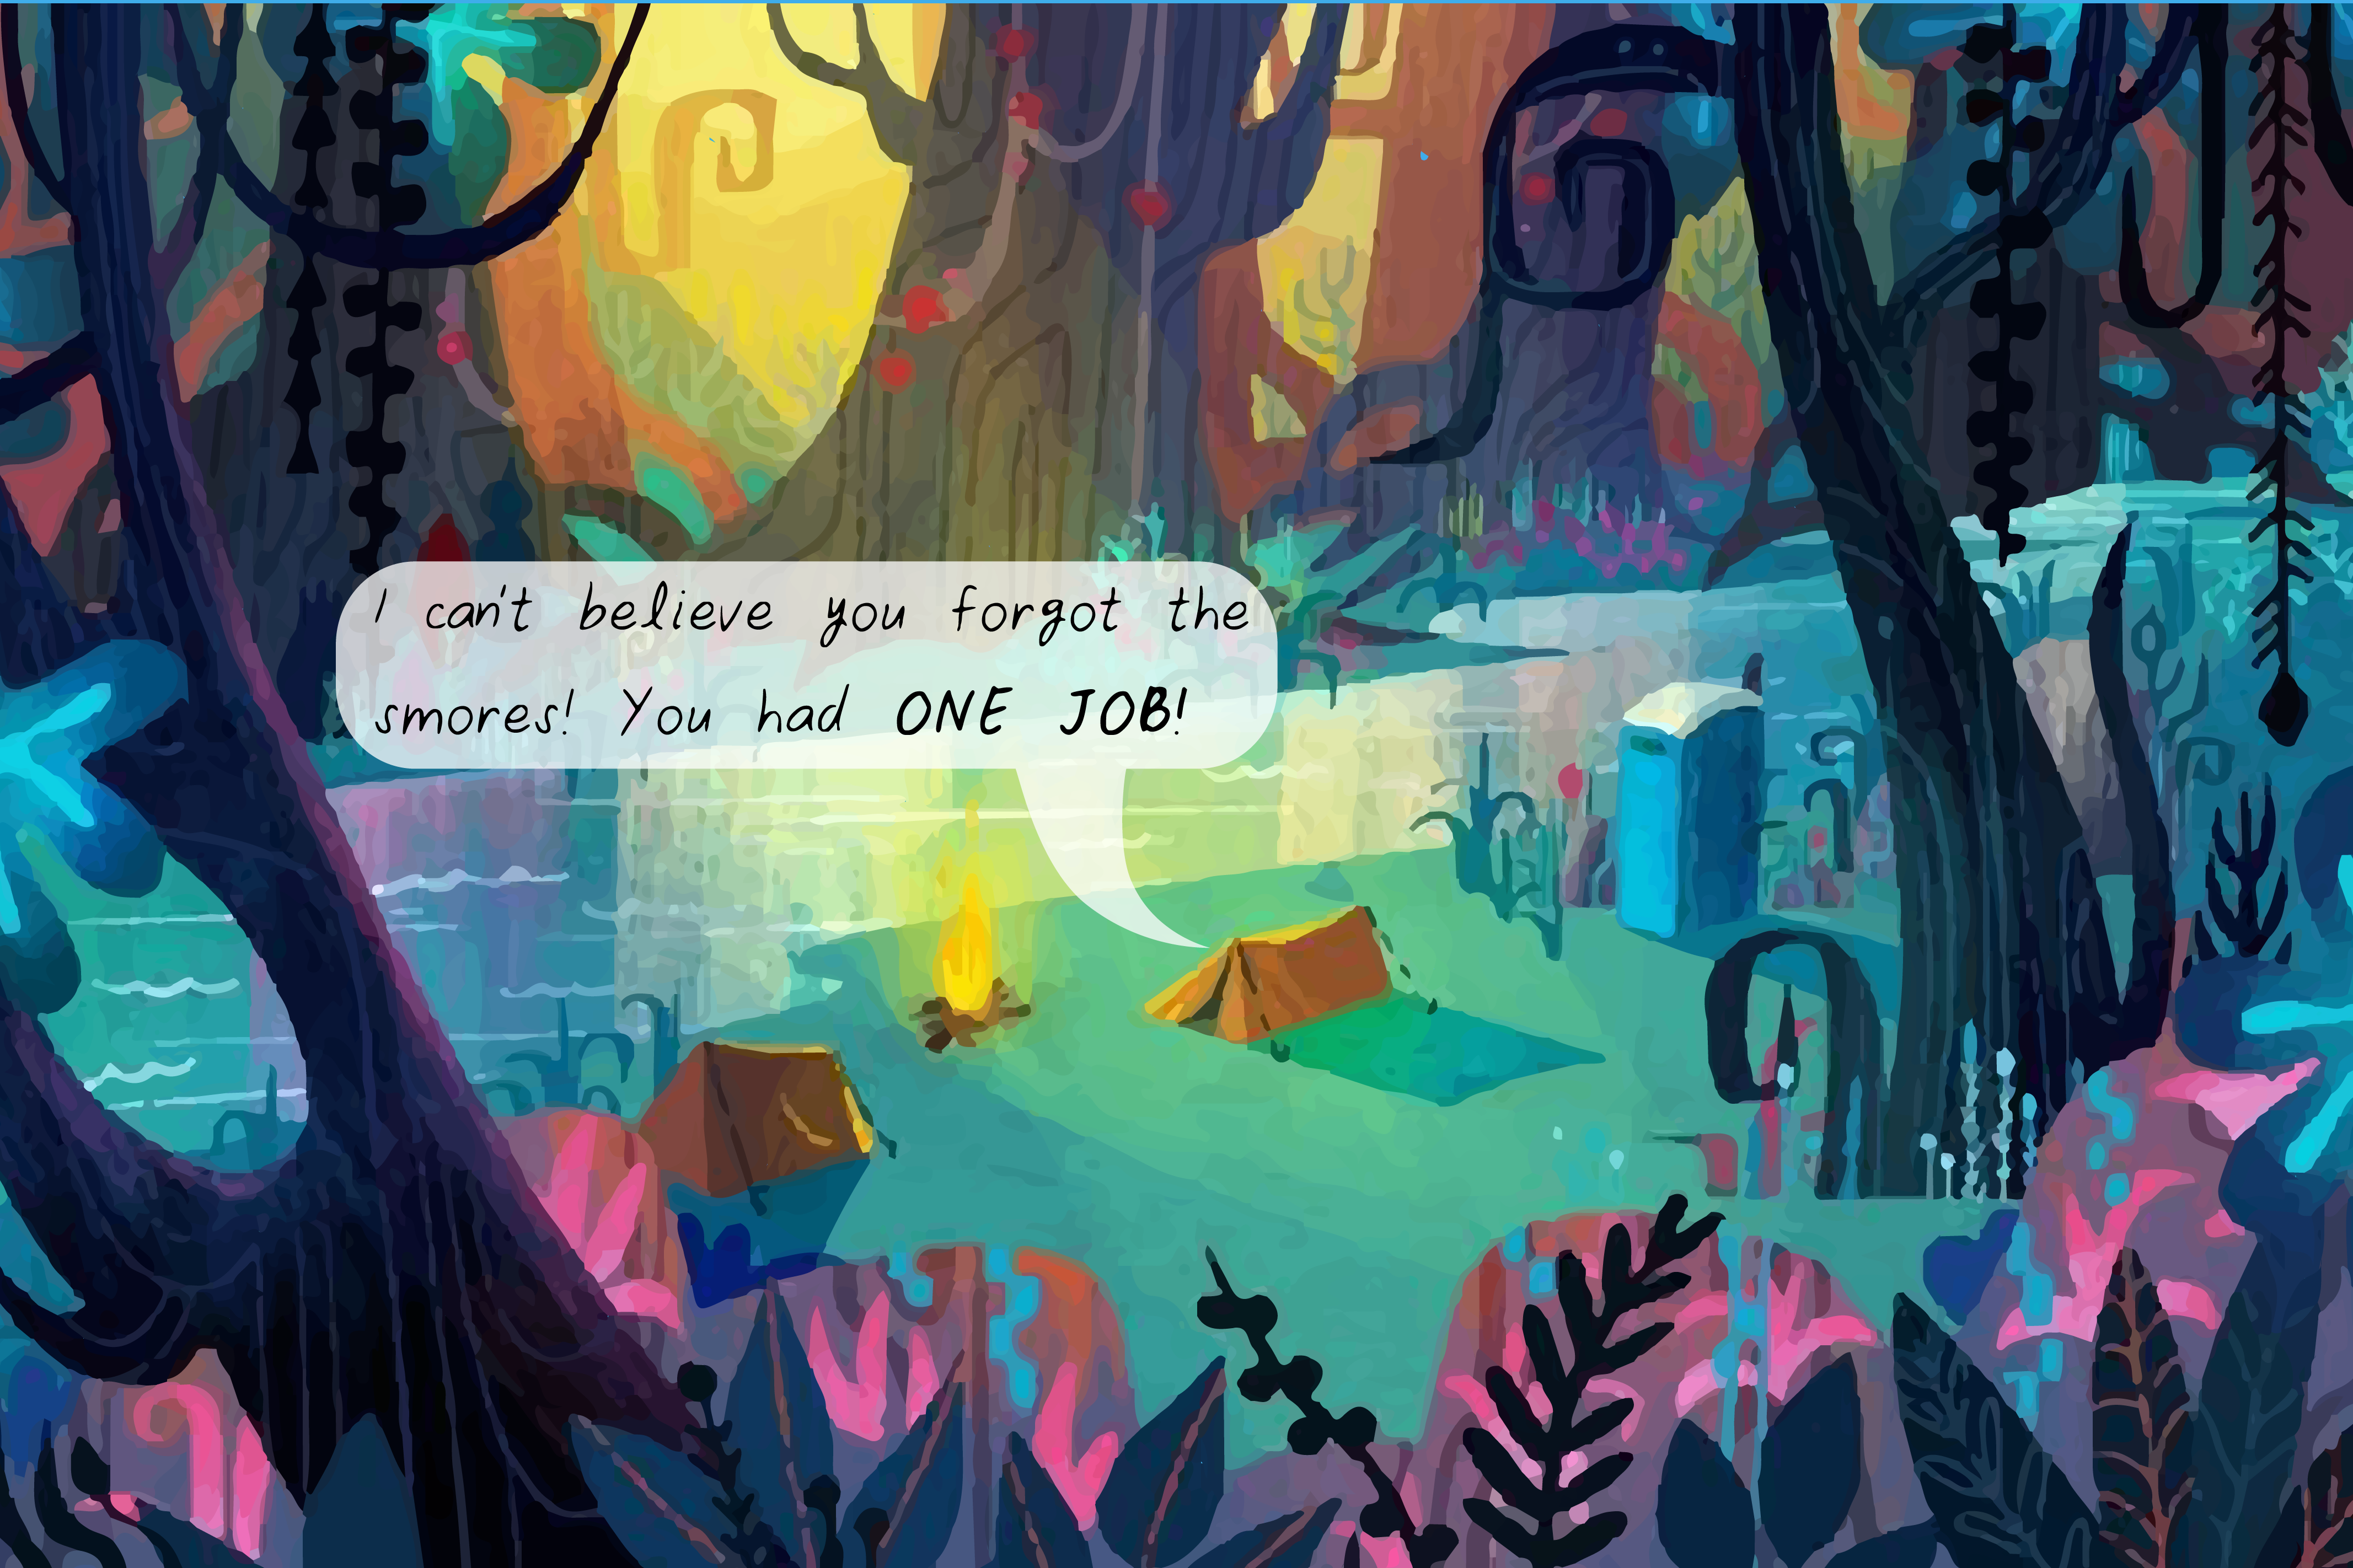
\includegraphics[width=2.5in]{figures/exp1/test-19.png} &
% 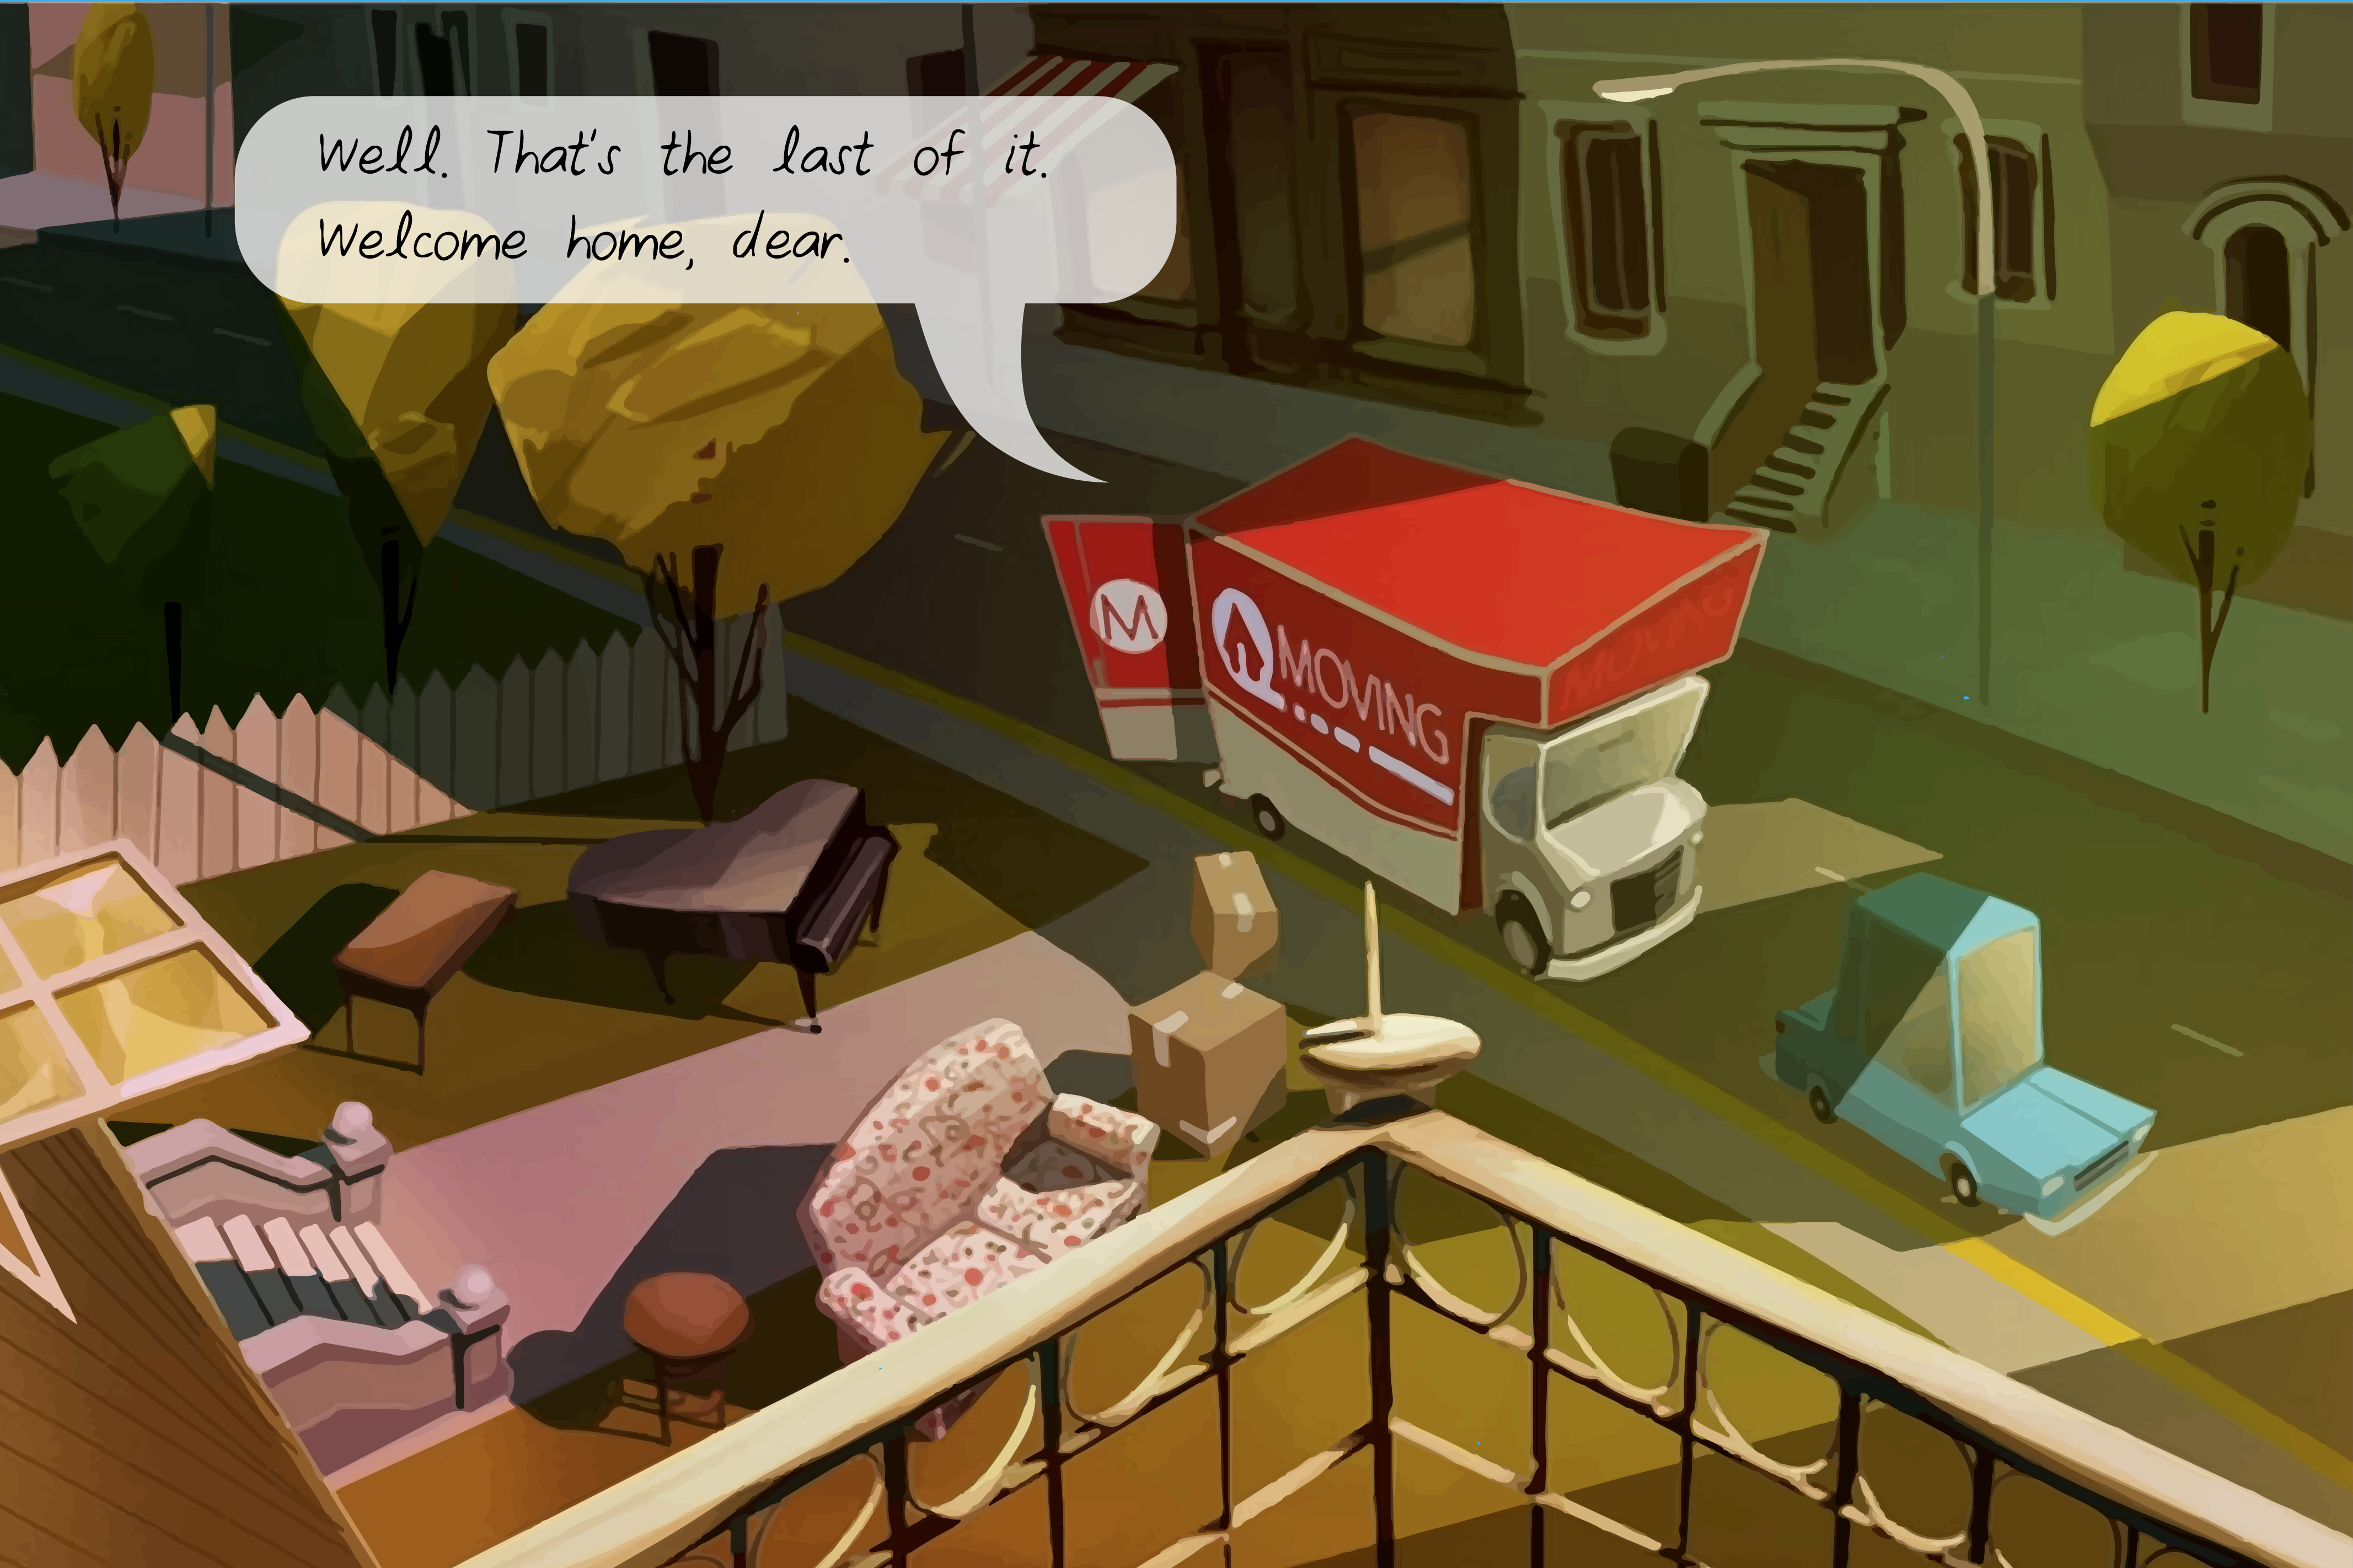
\includegraphics[width=2.5in]{figures/exp1/test-20.png}
% \end{array}$
% \end{center}
% \caption{Trial images from User Study 2, ctd.}
% \end{figure}



\section*{Appendix B: User Study 2}
\addcontentsline{toc}{section}{Appendix B: User Study 2}

% Confidence interval:
%   The mean of	none minus greens equals -0.418776725758
%   95% confidence interval of this difference: From -0.822466706937 to -0.015086744578 
% Intermediate values used in calculations:
%   t = 2.2602
%   df = 12

% \begin{table}[h!]
% \centering
%  \begin{tabular}{|m{5em} || m{6em} | m{10em} | m{10em}|} 
%  \hline
%  Group & Affect & Adjectives & Next Day Plans \\ 
%  \hline\hline
%  none & 0.0516810976 & "boodle boodle" & "poodle doodles" \\ 
%  none & 0.636986 & "devious" & "chomp will eat the other fish" \\
%  greens & 0.8030303 & "adorable, heartwarming, calming, Nemo-like, colorful, whimsical" & "ill be another shark stereotype misunderstanding that is also resolved" \\
%  greens & 0.720838249 & "Active, Outgoing, Determined" & "He will make more friends" \\
%  greens & 0.7200083 & "nervous, eager, determined. lonely, friendly, motivated, unrelenting" & "ill have a picnic/lunch party (something where they all eat together)." \\
%  none & 0.74491477 & "timid, lonely, scared, shy, cautious, unsure" & "thing new and make even more friends. probubly go on an adventure " \\
%  none & 0.5 & "Friendly" & "he will make a new friend " \\
%  none & 0.0566625558 & "Naive, friendly, innocent, slow" & "They will have to hunt for food / eat things" \\
%  none & 0 & "Smiley, Nice, Hungry" & "Chomp's going to eat more fish." \\
%  greens & 0.9906599 & "sad, lonely, misunderstood, nice, friendly" & "Chomps will have a better day with his new sea friends" \\
%  none & 0.156289 & "Shy, ruthless, deceptive" & "Chomp will eat more of his classmates" \\
%  none & 0.5 & "Friendly" & "He struggles with his natural hunting instincts" \\
%  none & 0.114778049 & "accidental fish eater" & "i think he's going to eat more fish by accident" \\
%  none & 0.0525114536 & "crafty" & "Chomp will eat more of the "children"" \\
%  none & 0.807181537 & "Friendly, shy, and loyal" & "more friends and enjoy Ms Pufferfish's lesson plan, no matter what it is. \\ [1ex] 
%  \hline
%  \end{tabular}
% \end{table}


% \begin{figure}[h]
% \begin{center}$
% \begin{array}{c c}
% \includegraphics[width=2.5in]{figures/exp2_screencaps/01.png} &
% \includegraphics[width=2.5in]{figures/exp2_screencaps/02.png} \\ 
% \includegraphics[width=2.5in]{figures/exp2_screencaps/03.png} &
% \includegraphics[width=2.5in]{figures/exp2_screencaps/04.png} \\ 
% \includegraphics[width=2.5in]{figures/exp2_screencaps/05.png} &
% \includegraphics[width=2.5in]{figures/exp2_screencaps/06.png} \\ 
% \includegraphics[width=2.5in]{figures/exp2_screencaps/07.png} &
% \includegraphics[width=2.5in]{figures/exp2_screencaps/08.png} \\ 
% \includegraphics[width=2.5in]{figures/exp2_screencaps/09.png} &
% \includegraphics[width=2.5in]{figures/exp2_screencaps/10.png}
% \end{array}$
% \end{center}
% \caption{Trial images from User Study 2}
% \end{figure}

% \begin{figure}[h]
% \begin{center}$
% \begin{array}{c c}
% 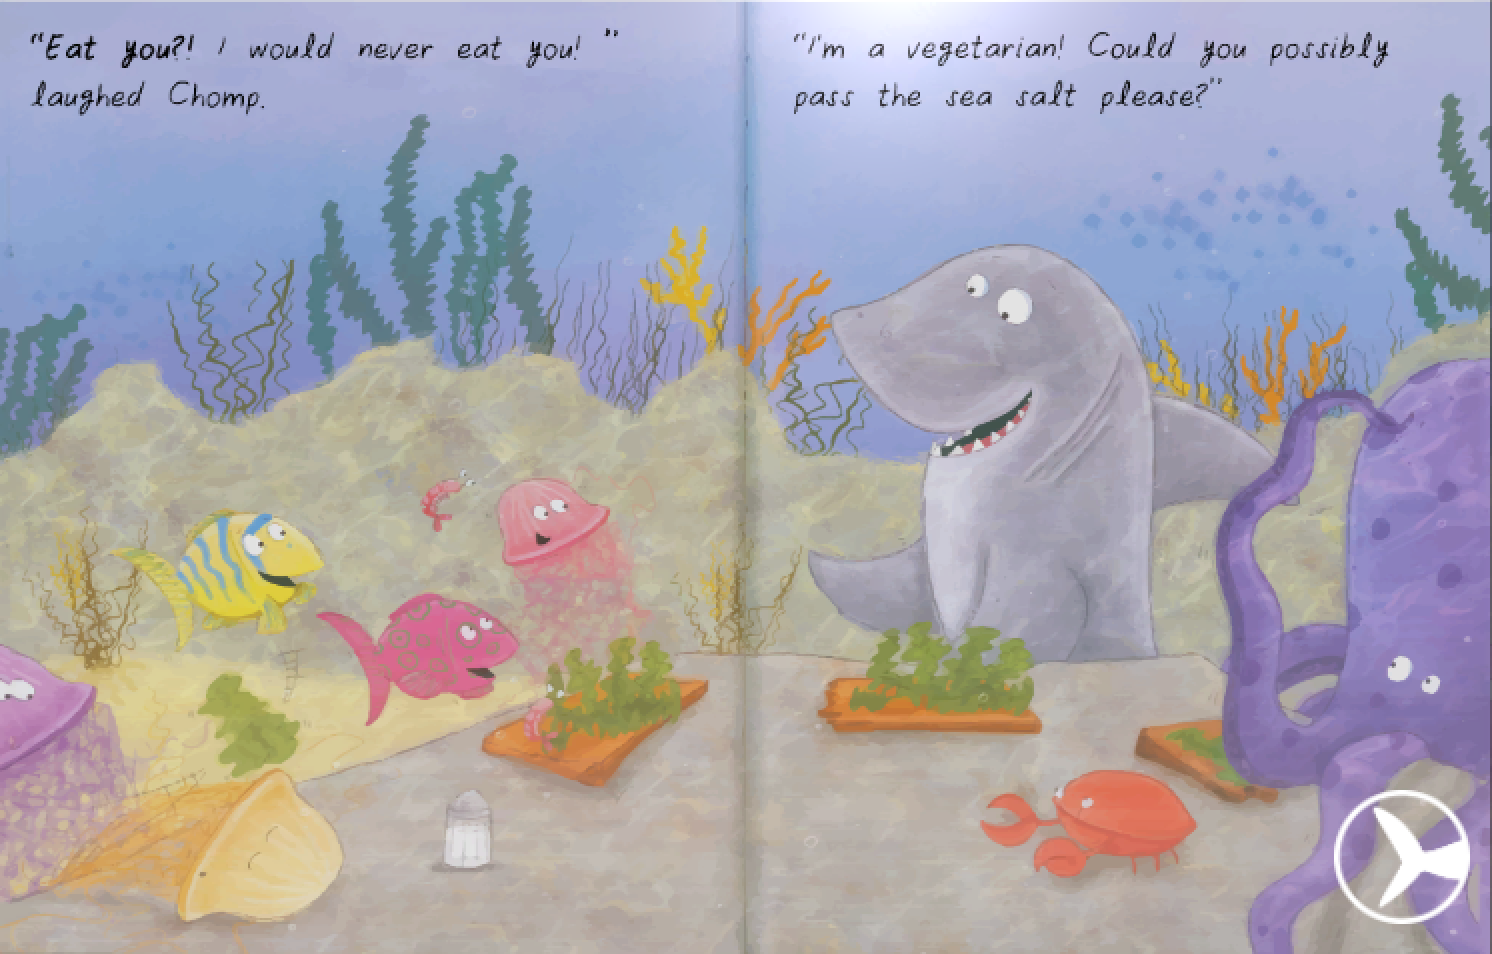
\includegraphics[width=2.5in]{figures/exp2_screencaps/11.png} &
% 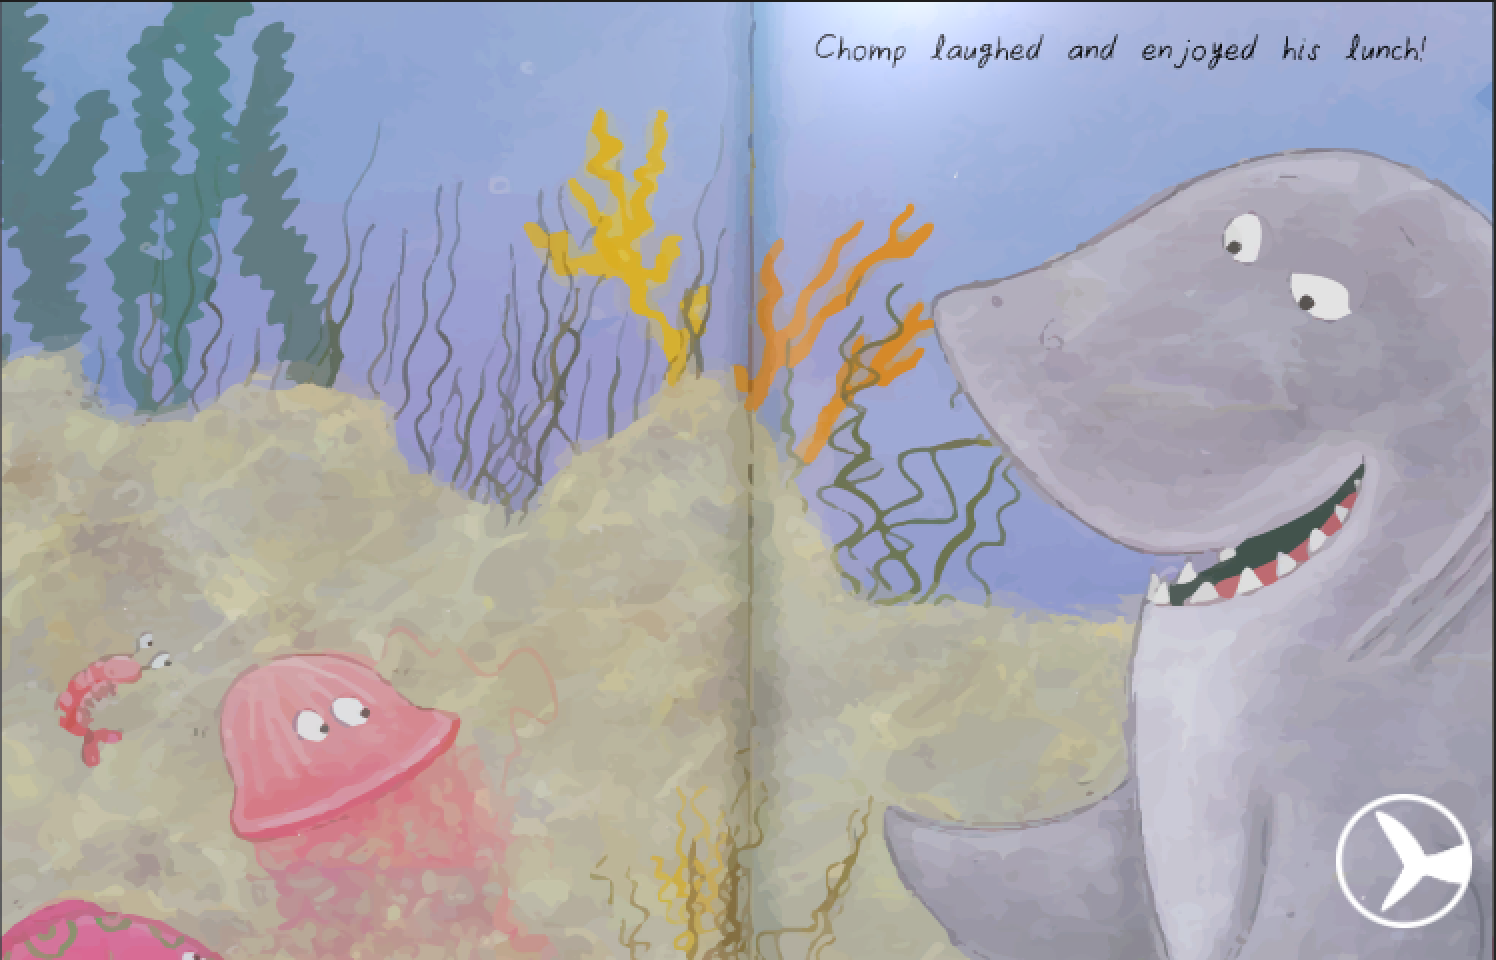
\includegraphics[width=2.5in]{figures/exp2_screencaps/11_alt.png} \\ 
% 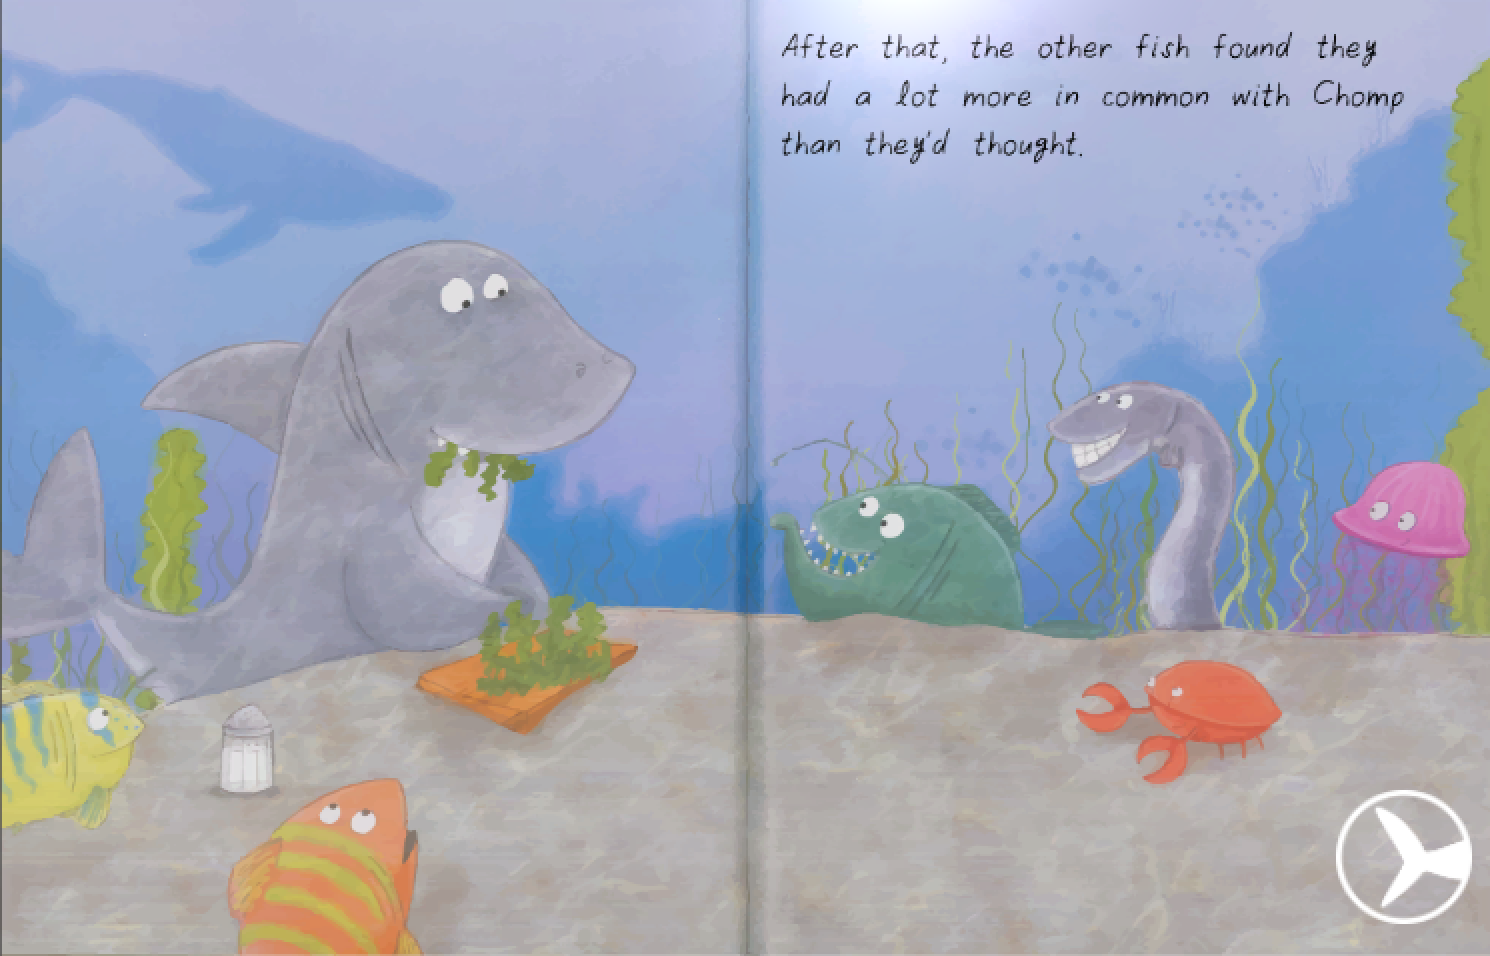
\includegraphics[width=2.5in]{figures/exp2_screencaps/12.png} &
% 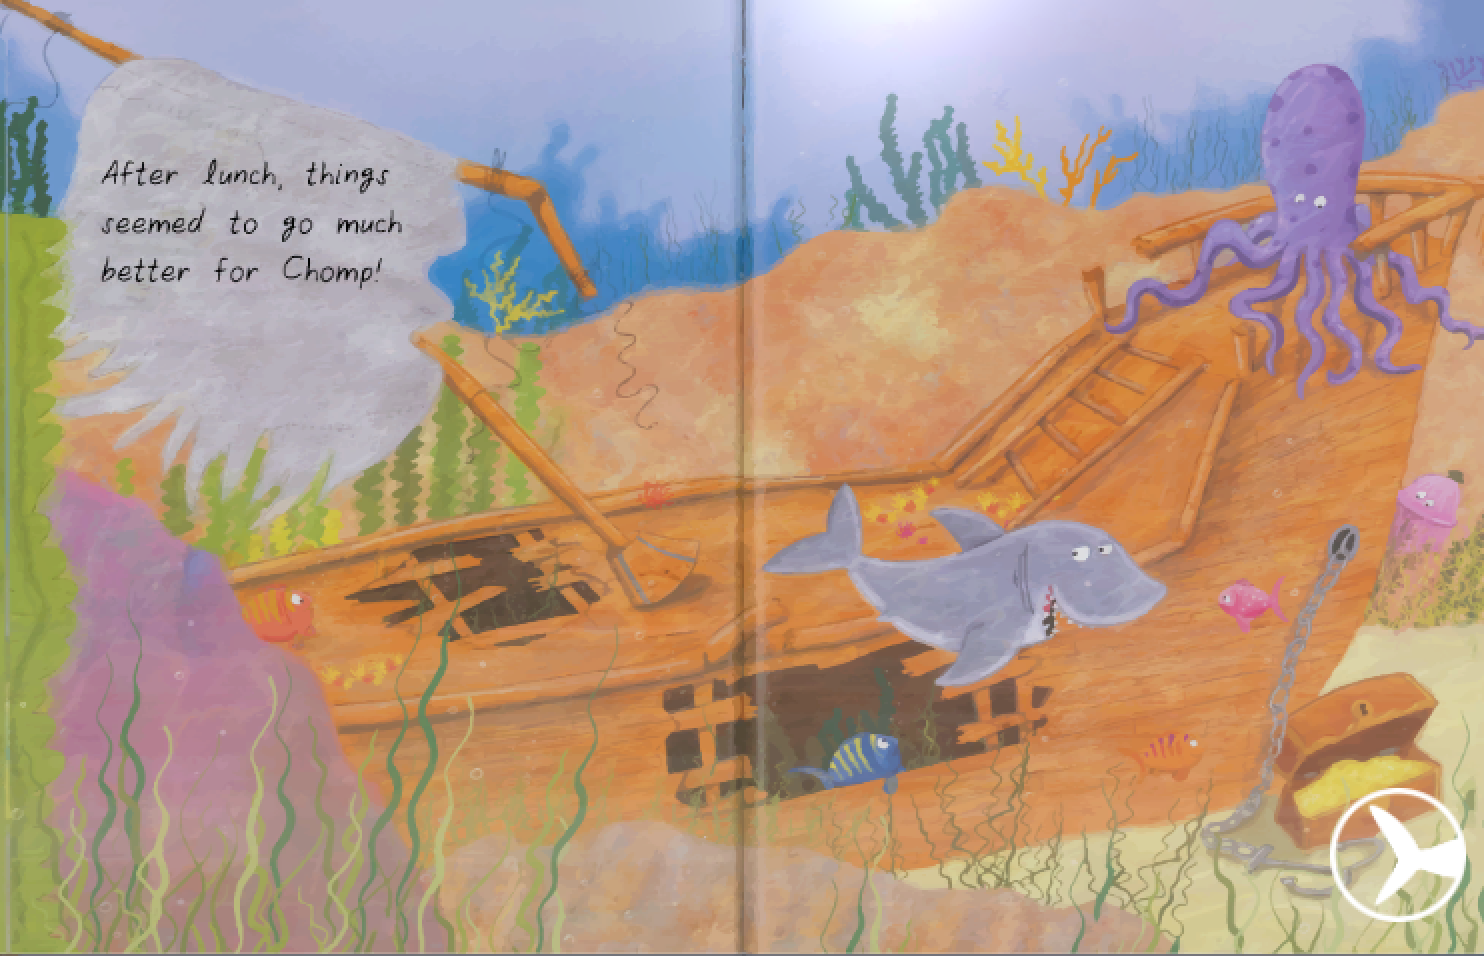
\includegraphics[width=2.5in]{figures/exp2_screencaps/13.png} \\ 
% 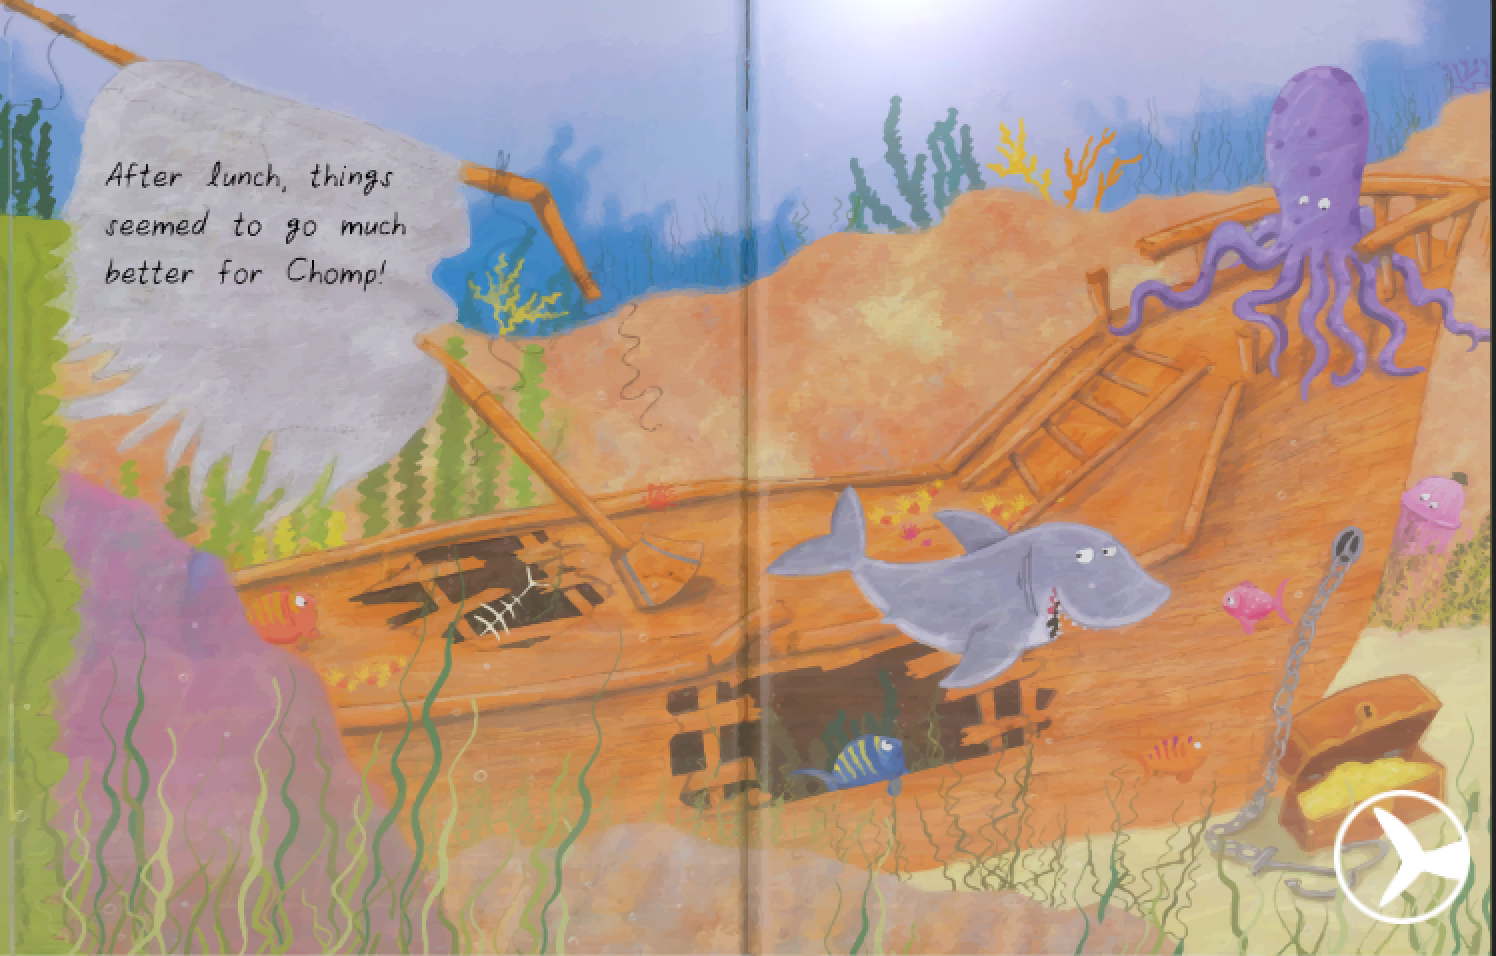
\includegraphics[width=2.5in]{figures/exp2_screencaps/13_alt.png} &
% 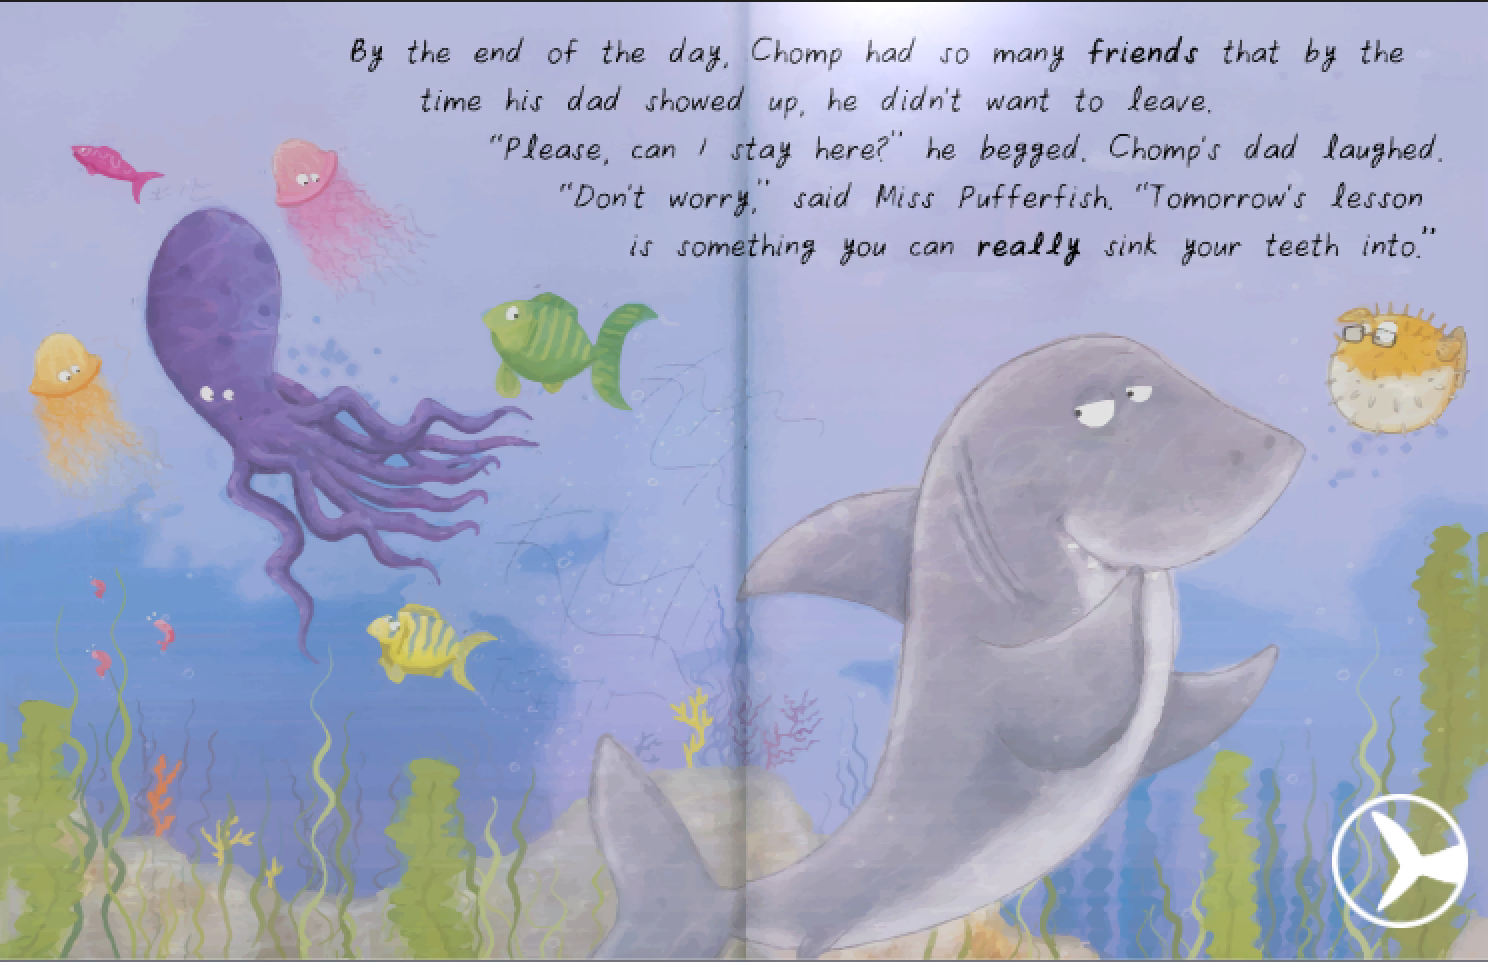
\includegraphics[width=2.5in]{figures/exp2_screencaps/14.png} \\ 
% 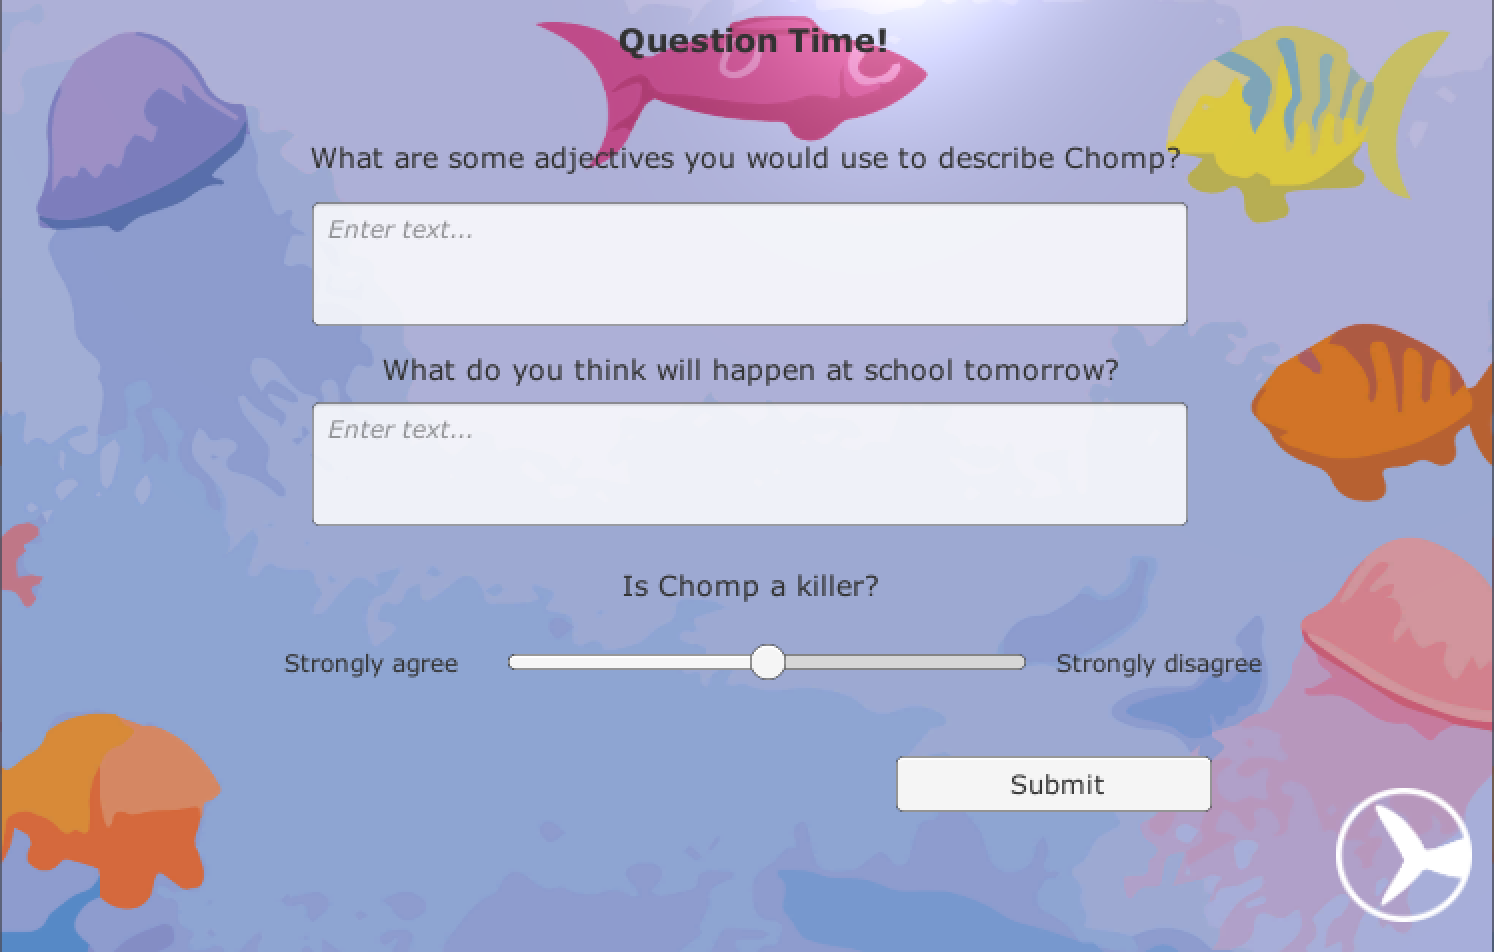
\includegraphics[width=2.5in]{figures/exp2_screencaps/15.png} &
% 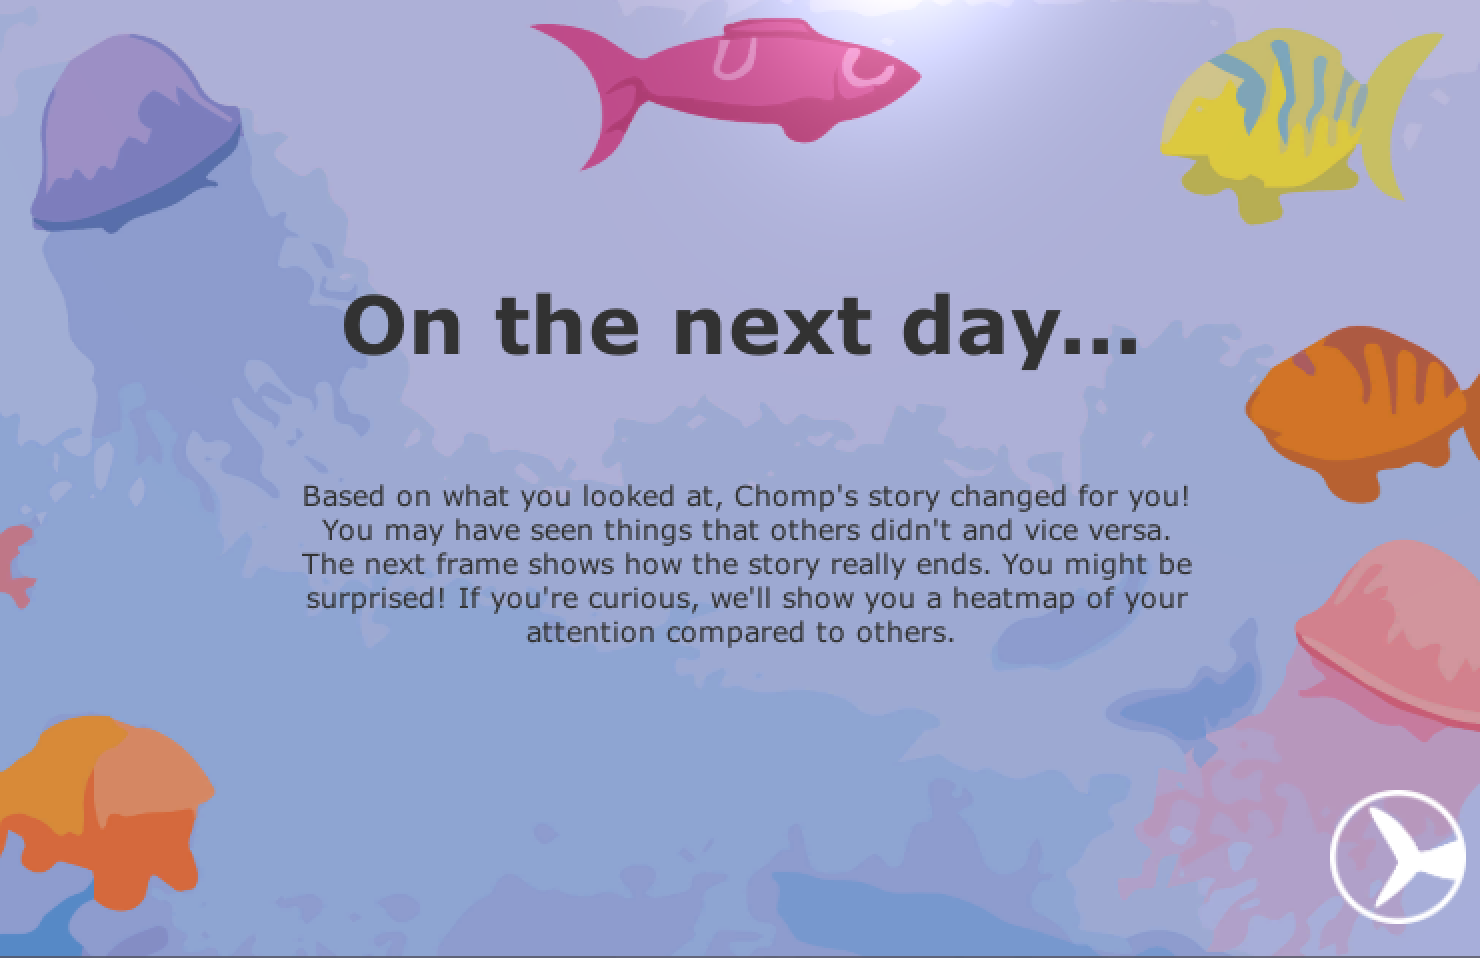
\includegraphics[width=2.5in]{figures/exp2_screencaps/16.png} \\ 
% 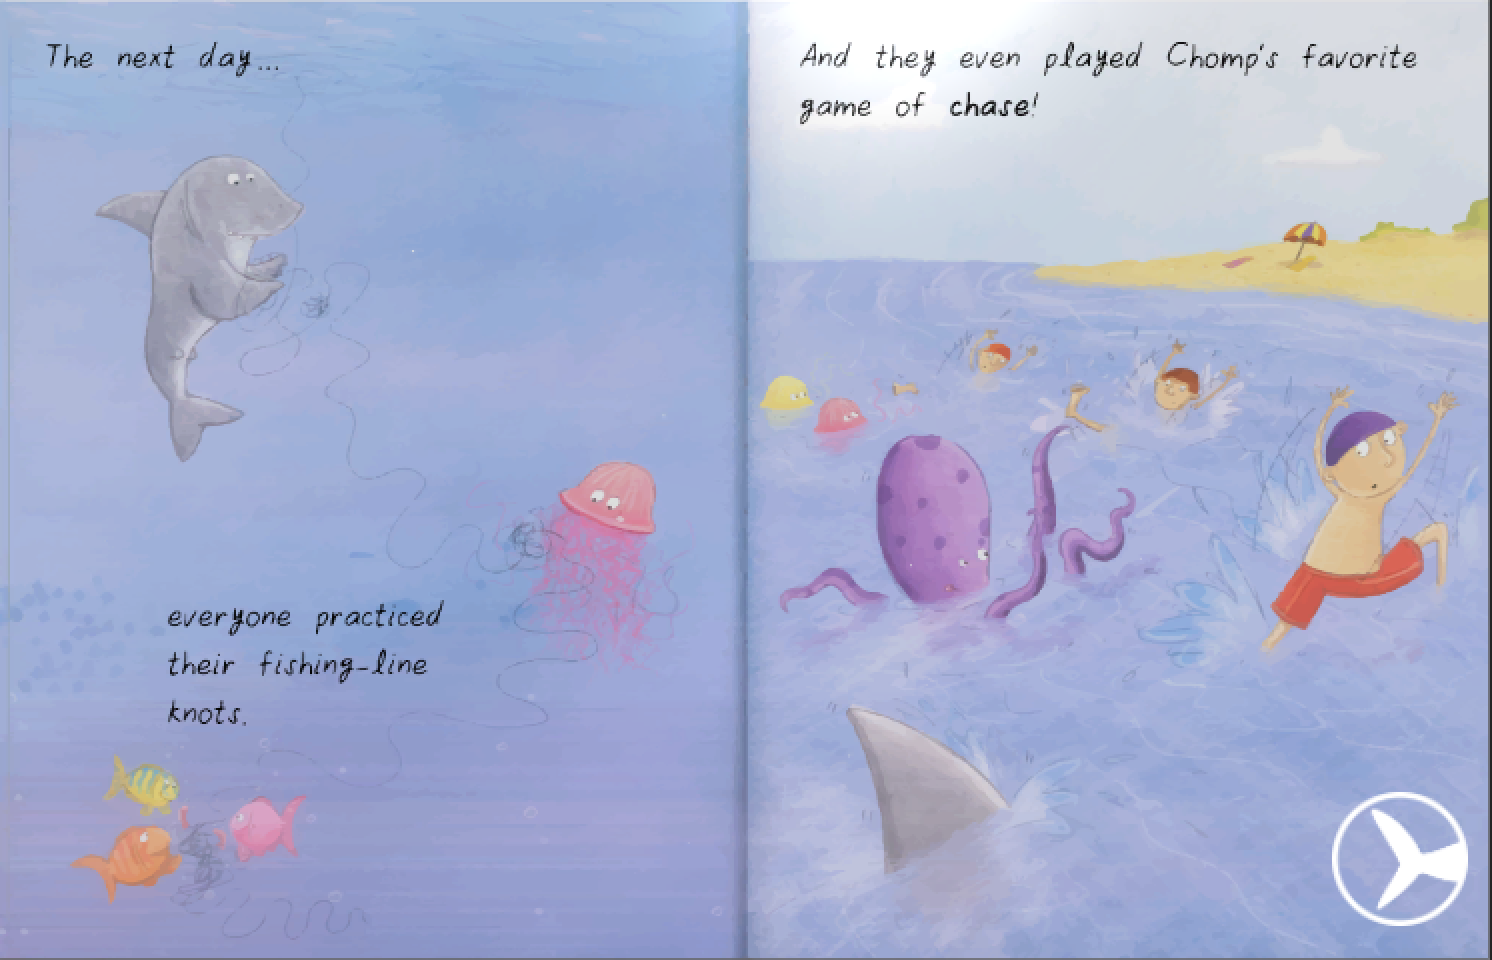
\includegraphics[width=2.5in]{figures/exp2_screencaps/17.png} &
% 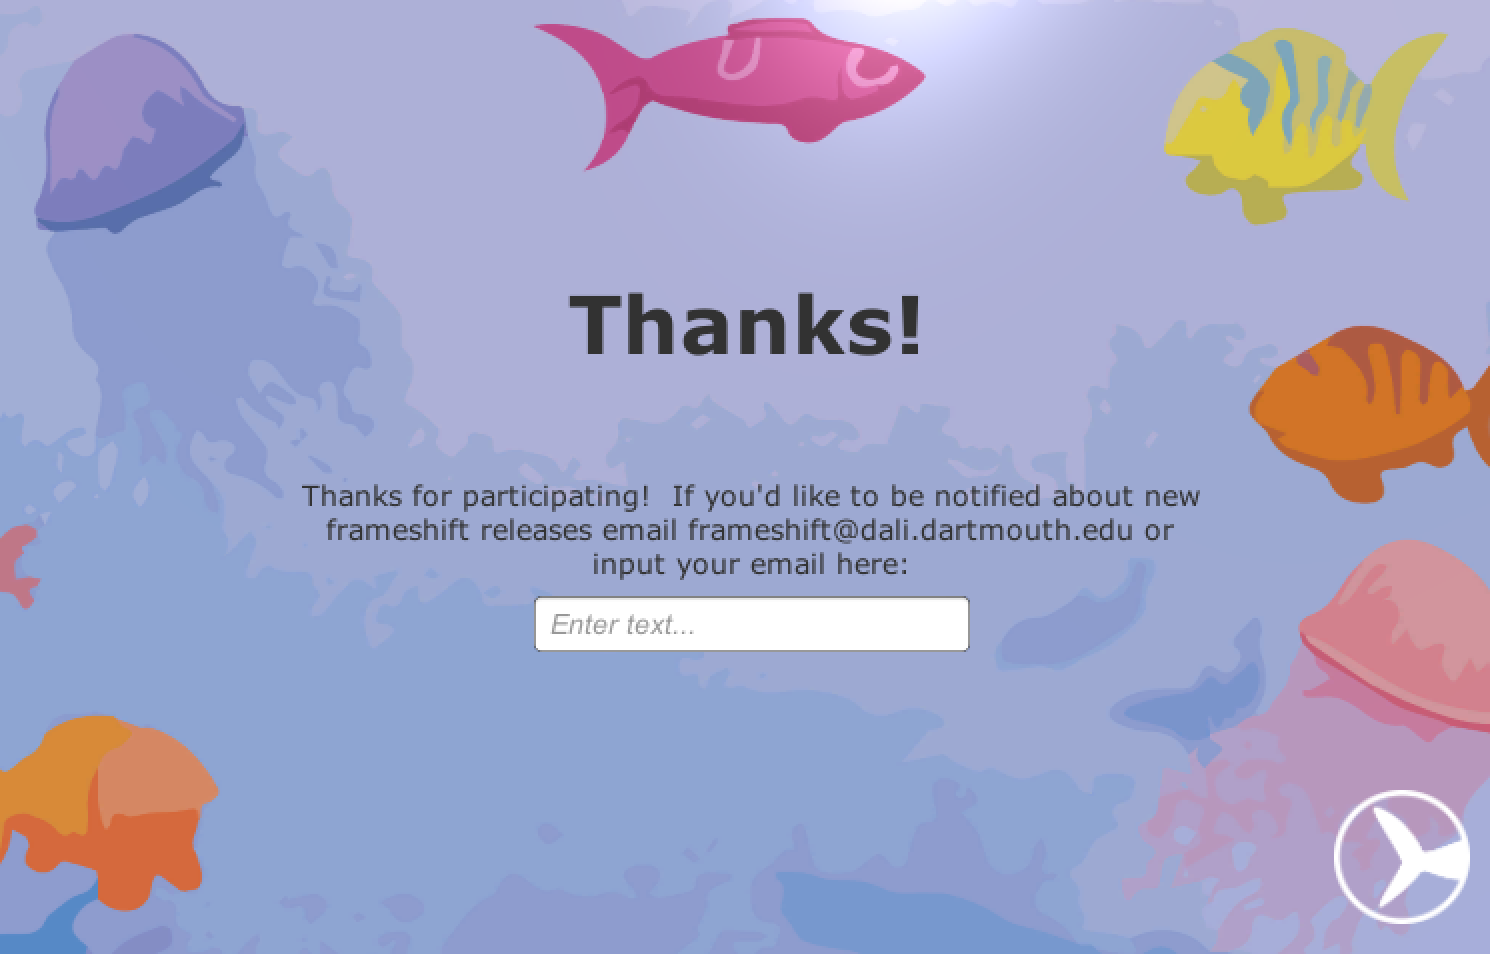
\includegraphics[width=2.5in]{figures/exp2_screencaps/18.png}
% \end{array}$
% \end{center}
% \caption{Trial images from User Study 2, ctd.}
% \end{figure}








\section*{Appendix C: Distribution of Work}
\addcontentsline{toc}{section}{Appendix C: Distribution of Work}

% As part of the requirement for a joint thesis this sections identifies the different work performed by each of the two authors. 

% Rukmini Goswami took the lead on:
% \begin{itemize}
%  \setlength\itemsep{-0.5em}
%  \item user study design and process
%  \item analysis of results
%  \item experimental setup in Unity3D
%  \item EyeTribe initial experimentation
%  \item statistical methods
%  \item all artwork for the future work
% \end{itemize}

% Tim Tregubov took the lead on: 
% \begin{itemize}
%  \setlength\itemsep{-0.5em}
%  \item scaffolding out the Unity3D C\# classes and framework. 
%  \item designing the narrative framework structure
%  \item Tobii SDK integration
%  \item gaze and fixation data processing
%  \item stack architecture and code structure
% %  \begin{itemize}
% %     \setlength\itemsep{-0.5em}
% %     \item for thi
% %  \end{itemize}
% \end{itemize}

 
\section*{Appendix D: Preview images from FrameShift the novel}
\addcontentsline{toc}{section}{Appendix D: Preview images from FrameShift — the novel}
% \begin{figure}[h!]
% \begin{center}$
% \begin{array}{c c}
% \includegraphics[width=2.3in]{figures/appendixD/01.png} &
% \includegraphics[width=2.3in]{figures/appendixD/02.png} \\ 
% \includegraphics[width=2.3in]{figures/appendixD/03.png} &
% \includegraphics[width=2.3in]{figures/appendixD/04.png} \\ 
% \includegraphics[width=2.3in]{figures/appendixD/05.png} &
% \includegraphics[width=2.3in]{figures/appendixD/06.png} \\ 
% \includegraphics[width=2.3in]{figures/appendixD/07.png} &
% \includegraphics[width=2.3in]{figures/appendixD/08.png} \\ 
% \includegraphics[width=2.3in]{figures/appendixD/09.png} &
% \includegraphics[width=2.3in]{figures/appendixD/10.png}
% \end{array}$
% \end{center}
% \end{figure}

\singlespacing

\bibliography{myrefs}
\addcontentsline{toc}{section}{Bibliography}



\end{document}
